\documentclass[spanish, 12pt, oneside]{Thesis}  
% Use the "Thesis" style, based on the ECS Thesis style by Steve Gunn
\usepackage[spanish,activeacute]{babel}
\graphicspath{ThesisFigs/}  % Location of the graphics files (set up for graphics to be in PDF format)
\usepackage[utf8]{inputenc}
% \usepackage{algorithm2e}
\usepackage[Algoritmo]{algorithm}
\usepackage{algorithmic}

% Include any extra LaTeX packages required
%\usepackage[square, numbers, comma, sort&compress]{natbib}  % Use the "Natbib" style for the references in the Bibliography
\usepackage[natbibapa]{apacite}
\usepackage{verbatim}  % Needed for the "comment" environment to make LaTeX comments
\usepackage{vector}  % Allows "\bvec{}" and "\buvec{}" for "blackboard" style bold vectors in maths
\hypersetup{urlcolor=black, colorlinks=true}  % Colours hyperlinks in blue, but this can be distracting if there are many links.
\usepackage{mathtools}
\usepackage{amsmath}
\usepackage{mathrsfs}
\usepackage{fancyhdr}
\usepackage{nomencl}
\usepackage{float}
\usepackage[left]{lineno}
\usepackage[titletoc]{appendix}
\usepackage{graphicx}
\usepackage{caption}
\usepackage{subfigure}
\usepackage[export]{adjustbox}
\usepackage{wrapfig}
\usepackage{standalone}
\usepackage{tikz}
\usetikzlibrary{shapes,arrows,calc,positioning}
\usetikzlibrary{babel}
\usepackage{color}
\usepackage{multirow}
\usepackage{enumitem}
\usepackage{listings}
\usepackage{rotating}
% Agregado para girar a horizontal una pagina.
\usepackage{pdflscape}
% Agregado para insertar pdf en latex.
\usepackage{pdfpages}
\definecolor{mylightblue}{RGB}{059,131,189}
\definecolor{mygreen}{RGB}{040,114,051}
\definecolor{myblue}{RGB}{062,095,138}
\definecolor{mygray}{RGB}{156,156,156}
\definecolor{myorange}{RGB}{255,128,0} 

\tikzstyle{intt}=[draw,text centered,minimum size=6em,text width=5.25cm,text height=0.34cm]
\tikzstyle{intl}=[draw,text centered,minimum size=2em,text width=2.75cm,text height=0.34cm]
\tikzstyle{int}=[draw,minimum size=2.5em,text centered,text width=3.5cm]
\tikzstyle{intg}=[draw,minimum size=3em,text centered,text width=6.cm]
\tikzstyle{sum}=[draw,shape=circle,inner sep=2pt,text centered,node distance=3.5cm]
\tikzstyle{summ}=[drawshape=circle,inner sep=4pt,text centered,node distance=3.cm]
\tikzstyle{decision} = [draw,shape=diamond, fill=blue!20, text width=6em, text badly centered, node distance=3cm, inner sep=0pt]

\usepackage{varioref}
\usepackage[tablename=Tabla]{caption}

\setlength\unitlength{20pt}


\usepackage{pst-plot}
\addtopsstyle{gridstyle}{gridlabels=0pt,griddots=0}
%% ----------------------------------------------------------------
\newcommand{\abbrlabel}[1]{\makebox[3cm][l]{\textbf{#1}\ }}
\newenvironment{abbreviations}{
    \begin{list}{}
    {
    \renewcommand{\makelabel}{\abbrlabel}
    \setlength\leftmargin{1.5in}
    \setlength\labelwidth{1.5in}
    }
}{
    \end{list}
}
%% ----------------------------------------------------------------

% Command to use grados
\newcommand{\grad}{$^{\circ}$ }

% -----------------------------------------------------------
\begin{document}

\maketitle
%% ----------------------------------------------------------------

\setstretch{1.3}  % It is better to have smaller font and larger line spacing than the other way round
\frontmatter      % Begin Roman style (i, ii, iii, iv...) page numbering
% Define the page headers using the FancyHdr package and set up for one-sided printing
\fancyhead{}  % Clears all page headers and footers
\rhead{\thepage}  % Sets the right side header to show the page number
\lhead{}  % Clears the left side page header

\pagestyle{fancy}  % Finally, use the "fancy" page style to implement the FancyHdr headers


%% --------------- Dedicatorias --------------------------------

\setstretch{1.3}  % Return the line spacing back to 1.3

\pagestyle{empty}  % Page style needs to be empty for this page
%\dedicatory{For/Dedicated to/To my\ldots}

\dedicatory{
Dedicatoria
% \begin{flushright}
% Dedico este trabajo a mis padres Luis y Felipa, que con su amor y trabajo me educaron y apoyaron en toda mi formación profesional. \newline
% A mis hermanas, por su apoyo incondicional y sus palabras de aliento en este largo trayecto recorrido.

% \textbf{Andrea}
% \end{flushright}


% \begin{flushright}
% Este trabajo va dedicado a mis padres, Ricardo Mora y Nilda Britos, mis pilares fundamentales a lo largo de mi formación profesional y personal. Gracias por todo.\newlin% % A mis compañeros y grandes amigos con quienes he pasado una gran parte de mi vida en estos años de formación profesional, gracias por el tiempo dedicado en los momentos que necesité.
% \newline
% Gracias a Dios y María, por ser una hija bendecida y permitirme culminar esta etapa para comenzar una nueva.

% \textbf{Francisco}
% \end{flushright}
}

 
   % Add a gap in the Contents, for aesthetics


%% --------------- Agradecimientos --------------------------------
% The Acknowledgements page, for thanking everyone
 \acknowledgements{
\addtocontents{toc}{\vspace{1em}}  % Add a gap in the Contents, for aesthetics

A la M.Sc. Ing María Elena García Vázquez, por la orientación y el tiempo que nos brindó ...


Al D.Sc. Ing. Luis G. Moré Rodríguez, por su apoyo en la búsqueda y recopilación de información, por su asesoramiento en la redacción y corrección de este libro; que han hecho posible la realización del presente trabajo.

Al D.Sc. Ing. Diego P. Pinto-Roa por sus charlas llenas de información, discusión y diferentes puntos de vista además de su apoyo general para la realización y culminación del proyecto.

Al M.Sc. Ing. José Luis Vázquez Noguera por la orientación y ayuda que nos brindó para la realización de esta tesis, por su apoyo incondicional desde el inicio del presente proyecto, que nos permitió aprender mucho más que lo estudiado en el proyecto.

A los tres, nuestros asesores de tesis, por el valioso tiempo que nos han dedicado para lograr este cometido. GRACIAS!

Un agradecimiento especial al M.Sc. Pedro Céspedes por prestarnos las computadoras del NIDTEC para realizar las ejecuciones de pruebas y por su paciencia y tiempo para encender dichas máquinas cada vez que se cortaba la energía eléctrica.

}
 \clearpage  % End of the Acknowledgements

%% --------------- Abstract ---------------------------------------

\addtotoc{Abstract}  % Add the "Abstract" page entry to the Contents
\abstract{
\addtocontents{toc}{\vspace{1em}}

\textit{TapeYty} is a tool developed to calculate optimal paths for urban garbage collection vehicles in the Asunción city. This tool generates benefits mainly in the economic and environmental aspects of the city where a large number of people brings a high generation of waste. This makes the complexity of garbage management even greater. 

The routing problem is treated as the directed open rural postman problem which seeks to minimize the distance to be traveled by the collection vehicles. To achieve the objective \textit{TapeYty} is based on mathematical programming techniques and Geographical Informatiom System (GIS) tool which allows the management of the route network, being able to update the road way and their state of blocked or nonblocked. This implies that when changes of street states are submitted  \textit{TapeYty} modifies the graph that represents the road network and re-calculates the solutions providing new optimal routes to each collection vehicle. 

The tool has provided solutions that save on average 20\% of distance compared to current tour.


% \textit{TapeYty} is a tool developed to calculate optimal paths for urban garbage collection vehicles in the Asunción city. This tool generates benefits mainly in the economic and environmental aspects of the city where a large number of people brings a high generation of waste. This makes the complexity of garbage management even greater. 

% The routing problem is treated as the open rural postman problem which seeks to minimize the distance to be traveled by the collection vehicles in its working area. To achieve the objective \textit{TapeYty} is based on mathematical programming techniques and Geographical Informatiom System (GIS) tool which allows the management of the route network to be able to update the road way and their state of blocked or nonblocked. This implies that when changes of state of the streets \textit{TapeYty} modifies the graph that represents the road network and re-calculates the solutions providing new optimal routes to each vehicle of collection. 

% The tool has provided solutions that save on average 20\% of distance traveled compared to current tour.
}
\clearpage  % Abstract ended, start a new page

%% --------------- Resumen --------------------------------------
\addtotoc{Resumen}  % Add the "Abstract" page entry to the Contents
\begin{resumen}
La mejora de contraste en imágenes a escala de grises es una técnica que busca resaltar la información útil de la imagen. Una de las técnicas utilizadas es el Contrast Limited Adaptive Histogram Equalization ($CLAHE$). Esta sin embargo, presenta un desafío en la selección de parámetros óptimos para realizar la mejora de contraste, los cuales pueden variar para cada instancia o imagen, además de la selección adecuada de las métricas para evaluar los resultados obtenidos.

En este trabajo se propone un estudio de distintas métricas disponibles en la literatura, de forma a definir en base a un estudio de correlación, cuáles de ellas serán utilizadas en un proceso de optimización multiobjetivo. Se aplica una  optimización Robusta basada en la metaheurística de enjambre de partículas ($SMPSO$), el cuál sintoniza los parámetros del algoritmo $CLAHE$, con el que se realiza la mejora de la imagen de manera a determinar las variables de decisión adecuadas para ciertos tipos de imágenes, y cuyos resultados se aproximen a los Frentes de Pareto de cualquier imagen del tipo estudiado, sin comprometer severamente la calidad de resultados con respecto a las optimizaciones de la mejora del contraste tomando como base imágenes individuales.

Se realizaron comparaciones de a pares entre métricas de mejora local y global, para medir la correlación entre ellas. Los resultados de la correlación obtenidos durante proceso de optimización muestran que las métricas \textit{Entropía Local} y el \textit{Índice de Similitud Estructural} ($SSIM$) tienen una alta correlación negativa por lo que el problema debe ser planteado en un contexto multiobjetivo.

% Además se observa que el $SMPSO$ es una herramienta factible para el cálculo de soluciones no dominadas sobre las cuales el algoritmo que toma las decisiones seleccionará la imagen más adecuada en base al contexto de trabajo.

Las pruebas experimentales realizadas muestran que es factible obtener Frentes de Pareto Robusto, para un grupo de imágenes del mismo tipo. Finalmente se compara el frente de Pareto robusto del grupo de imágenes analizado con cada uno de los frentes de Pareto de las imágenes individuales, de manera a demostrar experimentalmente la factibilidad de la propuesta.
\end{resumen}
\clearpage  % Abstract ended, start a new page
%% ----------------------------------------------------------------

\pagestyle{fancy}  %The page style headers have been "empty" all this time, now use the "fancy" headers as defined before to bring them back


%% --------------- Indice -----------------------------------------
\lhead{\emph{Contenido}}  % Set the left side page header to "Contents"
\tableofcontents  % Write out the Table of Contents

%% --------------- Lista de Figuras -------------------------------
 \lhead{\emph{Lista de Figuras}}  % Set the left side page header to "List if Figures"
\renewcommand\listfigurename{Lista de Figuras}
 \listoffigures  % Write out the List of Figures
 
  
%% --------------- Lista de Acrónimos -----------------------------
\addtotoc{Lista de Acrónimos}
\lhead{\emph{Acrónimos}}  % Set the left side page header to "Symbols"
\chapter*{Lista de Acrónimos\hfill}
\begin{abbreviations}
    \item[DSU] \textbf{D}irección de \textbf{S}ervicios \textbf{U}rbanos.
    \item[SWM] \textbf{S}olid de \textbf{W}aste \textbf{M}anagement.
    \item[TWL] \textbf{T}hreshold \textbf{W}aste \textbf{L}evel.
\end{abbreviations}

%% --------------- Lista de Símbolos ------------------------------
\addtotoc{Lista de Símbolos}
\lhead{\emph{Símbolos}}  % Set the left side page header to "Symbols"
\chapter*{Lista de Símbolos\hfill}

\begin{abbreviations}

    % cap 3
    \item[$XYZ$] Ejes de sistemas de coordenadas rectangulares.
    % \item[$J$] zona del hemisferio sur de UTM.
    \item[$(x, y)$] Par de coordenadas en un sistema vectorial.
    % cap4
    \item[$G$] Grafo.
    \item[$V$] Conjunto de vértices de un grafo.
    \item[$A$] Conjunto de enlaces de un grafo .
    \item[$A_R$] Arcos requeridos de un grafo.
    % \item[$E$] Conjunto de enlaces en G.
    % \item[$m$] Cantidad de vehículos.
    
    \item[$Q$] Capacidad de vehículos.
    \item[$q_{ij}$] Demanda no negativa del arco (i,j) en G.
    
    \item[$f$] Función objetivo de un problema de optimización.
    \item[$x$] Vector de variables.
    \item[$c$] Vector de restricciones.
    
    \item[$\mathbb{R}$] Conjunto de números reales.
    \item[$\mathbb{R}^n$] Espacio de n dimensiones de los números reales.
    \item[$\mathbb{Z}$] Conjunto de números enteros.
    \item[$\mathbb{Z}_{+}$] Conjunto de números enteros positivos.
    
    \item[$\mathcal{I}$] Conjunto de índices.
    \item[$\xi$] Conjunto de índices.
    % \item[$i$] Índices.
    
    \item[${S}$] Espacio solución factible.
    \item[$D$] Matriz.
    \item[$m$ x $n$] Dimensiones de la matriz D (m números de filas, n números de
    columnas).
    \item[$\mu$] Vector fila.
    \item[$b$] Vector columna.
    % \item[$x$] vector columna de variables.
    
    % cap5
    \item[$G'$] Grafo dirigido.
    \item[$H$] Grafo mixto.
    % \item[$G$] Grafo dirigido.
    % \item[$V$] Conjunto de vértices del grafo G.
    % \item[$A$] Conjunto de arcos dirigidos de la grafo G.
    \item[$E$] Subconjunto de A. Representan segmentos de calles de dos vías que pueden ser recorridos en cualquier sentido.
    \item[$(i,j)$] Representa un arco de A (segmentos de calle).
    \item[$AM$] Subconjunto de A. Segmentos de calles que deben recorrerse únicamente en el sentido especificado.
    \item[$w$] Función de peso que asocia un peso a cada arco de A.
    \item[$I$] Subconjunto de V. Posibles puntos iniciales de una ruta.
    \item[$\mathcal{S}$] Subconjunto de $V$.
    \item[$V \backslash \mathcal{S}$] Subconjunto de $V$ que no pertenecen a $\mathcal{S}$.
    \item[$\delta^+ (\mathcal{S})$] Subconjunto de A que van desde vértices en $\mathcal{S}$ a vértices en $V \backslash \mathcal{S}$.
    \item[$x_{i j}$] Número de veces que un arco de A es atravesado en una ruta.
    \item[$s_i$] Especifica si un vértice en I es el primer nodo en una ruta.
    \item[$t_j$] Especifica si un vértice en V es el último nodo en una ruta.
    \item[$R$] Modelo relajado utilizado en la solución propuesta.
    \item[$T$] Subtour en el grafo $G'$.
    \item[$P$] Camino principal.
    
    \item[$MG$] Multigrafo dirigido.
    \item[$O$] Notación O grande.
    \item[$N$] número de vértices en MG.
    \item[$M$] número arcos en MG.
    
    
    % % cap2
    % \item[$(i,j)$] Coordenadas espaciales de una imagen.
    % \item[$F(i,j)$] Imagen definida como función de dos dimensiones.
    % \item[$f(i,j)$] Imagen digital.
    % \item[$f'(i,j)$] Imagen modificada al aplicar una técnica de mejora de contraste.
    % \item[$M$ x $N$] Dimensiones de una matriz (M números de filas, N números de columnas.
    % \item[$(c,l)$] Índices de M y N.
    % \item[$p$] Píxel de una imagen.
    % \item[$\mathcal{H}$] Histograma de una imagen.
    % \item[$L$] Cantidad total de niveles de gris disponibles en una imagen.
    % \item[$L-1$] Nivel máximo de gris en una imagen.
    % \item[$k$] Nivel de gris o k-ésimo nivel de gris.
    % \item[$k'$] Nuevo nivel de gris mapeado por la ecualización del histograma.
    % \item[$n_k$] Número de ocurrencia de la intensidad k en la imagen.
    % \item[$Z$] Cantidad total de píxeles de una imagen.
    % \item[$\mathcal{R}$] Region contextual de una imagen.
    % \item[$(\mathcal{R}_i,\mathcal{R}_j)$] Tamaño de una Region contextual de una imagen.
    % \item[$\mathscr{C}$] Clip Limit usado por el Algoritmo $CLAHE$.
    
    % % cap3
    % \item[$P^*$] Conjunto Pareto Óptimo.
    % \item[$FP^*$] Frontera Pareto.
    % \item[$\Omega$] Región de soluciones factibles para el conjunto Pareto Óptimo.
    % \item[$\rho$] Una partícula del enjambre.
    % \item[$\chi _i$] Vector que almacena la posición actual de cada partícula.
    % \item[$\rho{Best_i}$] Vector que almacena la posición de la mejor solución encontrada por la partícula $i$ hasta el momento.
    % \item[$v_i$] Vector que almacena la velocidad actual de cada partícula.
    % \item[$t$] Número de iteraciones del algoritmo $PSO$.
    % \item[$v^{t}_i$] Velocidad de la partícula $i$ en la iteración $t$.
    % \item[$\omega$] Coeficiente de inercia del $PSO$.
    % \item[$\varphi_1$] Máximo valor que puede alcanzar el coeficiente cognitivo del $PSO$.
    % \item[$\varphi_2$] Máximo valor que puede alcanzar el coeficiente social del $PSO$.
    % \item[$\chi^{t}_i$] Posición actual de la partícula $i$ en la iteración $t$.
    % \item[$g_i$] Posición de la partícula con el mejor $fitness_{\rho{Best_i}}$ del entorno de $\rho_i$ o de todo el enjambre.
    % \item[$\kappa$] Coeficiente de restricción aplicado a $v^{t}_i$.
    
    
    % %cap4
    % \item[$\mathcal{P}_k$] Probabilidad de ocurrencias del nivel de gris $k$ en el histograma utilizado para el cálculo de $\mathscr{H}$.
    % \item[$\nu_{ij}$]   Representa una vecindad de una imagen.
    % \item[$\mathscr{H}$] Entropía.
    % \item[$\mathscr E$] Entropía Local.
    
    %  % cap5
    %  \item[$\gamma$] Coeficiente de correlación.
    %  \item[$I_f$ y $S_f$] Funciones objetivos de la propuesta.
     
    % \item[$\overrightarrow{x}$] Vector que almacena los valores de [$\mathcal{R}_i$, $\mathcal{R}_j$, $\mathscr{C}$].
    % \item[$\Re$] Frente Pareto Robusto.
    % \item [$\mathscr X$] Conjunto de soluciones no dominadas.
    % \item[$\Gamma$] Frente Pareto.
    % \item[$I$] Conjunto de imágenes.
    % \item[$\alpha$] Conjunto de soluciones óptimas de $I$ analizadas.
    % \item[$\beta$] Promedio de las soluciones óptimas originales de las imagenes.
    % \item[$\delta$] Promedio de soluciones óptimas entre todas las imagenes analizadas.
    
\end{abbreviations}

%% --------------- Lista de Tablas --------------------------------
 \lhead{\emph{Lista de Tablas}}  % Set the left side page header to "List of Tables"
 \renewcommand\listtablename{Lista de Tablas}
 \listoftables  % Write out the List of Tables
 
%% --------------- Contenido -----------------------------------
\clearpage
\mainmatter	  % Begin normal, numeric (1,2,3...) page numbering
\pagestyle{fancy}  % Return the page headers back to the "fancy" style
% Include the chapters of the thesis, as separate files
% Just uncomment the lines as you write the chapters

\lhead{\emph{Introducción}} 
\renewcommand\chaptername{Capítulo}%título "Capítulo"
\chapter{Introducción}

Las imágenes digitales están expuestas a sufrir una variedad de distorsiones durante su procesamiento, compresión, almacenamiento, transmisión y reproducción, cualquiera de estas puede resultar en la degradación de la calidad visual \cite{digitalimganalysis}.

Aunque el campo de procesamiento digital de imágenes está construido sobre una base de formulaciones matemáticas y probabilísticas, la intuición y el análisis humano juegan un papel central en la elección de una técnica frente a otra. Esta elección se hace a menudo sobre la base de juicios subjetivos visuales, por lo tanto, se necesitan conseguir medidas cuantitativas que puedan valorar de forma objetiva la calidad de la imagen percibida.

El proceso digital de imágenes se puede dividir en las siguientes áreas \cite{digitalimageprocessing}:
\begin{itemize}
\item \textbf{Adquisición o captura} que se ocupa de los diferentes caminos para la obtención de imágenes; por ejemplo, utilizando cámaras digitales o digitalizando imágenes impresas (fotografías).
\item \textbf{Realce y mejora} son las técnicas que se usan para mejorar condiciones de bajo contraste, baja luminosidad o demasiada oscuridad. Ejemplo: ecualización de histograma.
\item \textbf{Segmentación} que se ocupa de la división de las imágenes en regiones o áreas significativas.
\item \textbf{Extracción de características} que se ocupa de la detección y localización de entidades geométricas simples y complejas. Desde entidades simples como líneas y puntos hasta geometrías complejas como curvas y cuádricas.
\end{itemize}

El objetivo principal de las técnicas de realce y mejora de imagen es procesar una imagen, ya sea en contraste, ruido, escala de grises, distorsiones, luminosidad, falta de nitidez, etc., o bien convertir o mapear la imagen de forma que resulte más adecuada que la original para una aplicación específica.

Existen diversas técnicas para llevar a cabo el mejoramiento de contraste en una imagen. Estas técnicas pueden ser divididas en 2 grandes clases. La primera clase implica la descomposición de la imagen en altas y bajas frecuencias y en la combinación de éstas dos señales independientes \cite{kober2002unsharp}. El filtrado homomórfico y el “unsharp masking” son ejemplos de esta clase. La segunda clase consiste en la modificación del histograma de la imagen como la técnica de ecualización del histograma.

La ecualización del histograma de una imagen \textit{HE} \cite{PTS+13} es ampliamente utilizado como herramienta tanto cualitativa como cuantitativa, es una buena herramienta para la mejora de contraste. Sin embargo, este método de mejora de contraste puede producir imágenes de aspecto no natural, lo que ocasiona que las imágenes obtenidas no sean las más adecuadas. Existen enfoques de mejora global y local \cite{morebrizuela2014}. Si se usa sólo información global, no se alcanza un buen realce de contraste debido a que las técnicas globales podrían causar un efecto de saturación de intensidades. Los enfoques locales consideran una ventana local para cada píxel y calculan el valor de la nueva intensidad basados en el histograma local definido. Todos los pixeles de una ventana local contribuyen igualmente a la determinación del nuevo valor del píxel central que está siendo considerado, solucionando el problema que podrían presentar los enfoques globales \cite{yu2004fast}. 

Entre las técnicas de mejoras de contraste basadas en \textit{HE}, encontramos técnicas de optimización con el uso de Algoritmos Genéticos \cite{hashemi2010image}, la Lógica Difusa \cite{jenifer2016contrast}, Optimización por Enjambres de Partículas con parámetros del Contrast Limited Adaptive Histogram Equalization \textit{PSO-CLAHE} \cite{morebrizuela2014}.

El objetivo de la optimización es encontrar una solución que represente el valor óptimo para una función objetivo. La optimización multi-objetivo no se restringe a la búsqueda de una única solución, sino de un conjunto de soluciones que representan los mejores compromisos entre los distintos criterios, llamados \textbf{soluciones no-dominadas} o \textbf{conjunto Pareto Óptimo} con el fin de ofrecer al tomador de decisiones (Decision Maker - DM) las mejores alternativas entre las disponibles, para que este último seleccione una de ellas \cite{coello2001short}.

La principal finalidad de la optimización multi-objetivo robusta es la obtención del \textbf{Frente de Pareto} de un conjunto de imágenes, tomados como una sola entrada, cuyos resultados se aproximen a los \textbf{Frentes de Pareto} de cualquier imagen de manera individual del tipo estudiado, sin comprometer severamente la calidad de los resultados \cite{Deb2006IntroducingRI}.

En la literatura, los enfoques de mejora local demuestran ser sumamente útiles al momento de resaltar detalles en imágenes con gran cantidad de detalles finos. Debido a ello en esta propuesta se analizan pares de métricas de calidad, junto a una metaheurística de optimización de objetivos \textit{SMPSO} \cite{RC05}, de manera a sintonizar los parámetros de entrada del algoritmo de mejora del contraste \textit{CLAHE}. Obteniendo como resultado un grupo de imágenes contrastadas, las cuales serán evaluadas en cuanto a la ganancia de información proveída y distorsión introducida por la ecualización, así también se realiza una comparación de la correlación entre las métricas seleccionadas para identificar las más adecuadas para la optimización multi-objetivo de la mejora de contraste.


\section{Objetivo General}
El objetivo general de este trabajo de investigación es el estudio de distintas métricas disponibles, para la evaluación de la calidad de las imágenes, de forma a definir en base a un estudio de correlación, cuáles de ellas serán utilizadas en un proceso de optimización multiobjetivo.
% El objetivo general de este trabajo de investigación es el estudio de distintas métricas de evaluación de calidad de imágenes disponibles, de forma a definir en base a un estudio de correlación, cuáles de ellas serán utilizadas en un proceso de optimización multiobjetivo.


\section{Objetivos Específicos}

Los objetivos específicos que se han trazado en este trabajo para lograr el objetivo general son:
\begin{itemize}
  %  \item \textbf{Reportar} los principales trabajos de la literatura que abordan el problema estudiado.
    \item \textbf{Seleccionar un conjunto de métricas} para evaluar la ganancia o pérdida de información y distorsión en una imagen.
    \item \textbf{Aplicar una metaheurística} para sintonizar los parámetros del algoritmo \textit{CLAHE}.
    \item \textbf{Aplicar al conjunto de soluciones la correlación de Pearson} para medir el grado de relación o covariación entre las métricas.
    \item \textbf{Comparar los resultados obtenidos de la correlación de Pearson} y de esta forma obtener las métricas más apropiadas para el proceso de optimización.
    \item \textbf{Proponer} un algoritmo multiobjetivo, tal que opere en conjunto con el \textit{CLAHE} y las métricas de evaluación de calidad seleccionadas, sobre un conjunto de imágenes para obtener las imágenes mejoradas.
\end{itemize}


\section{Organización del Trabajo}

El resto del trabajo se organiza de la siguiente manera:

\begin{itemize}
    \item En el \textbf{capítulo 2} se presentan los conceptos básicos que describen a la mejora de imagen y la mejora de contraste como también el algoritmo \textit{CLAHE}.
    \item En el \textbf{capítulo 3} se presenta la metaheurística de optimización de enjambre de partículas escogida para encontrar los parámetros óptimos del algoritmo \textit{CLAHE}.
    \item En el \textbf{capítulo 4} se presentan las métricas de evaluación de soluciones utilizadas para el analisis de investigación de este trabajo.    
    \item En el \textbf{capítulo 5} se plantea de manera formal el problema que se intenta resolver. Cómo se utilizan las métricas seleccionadas para la evaluación de los resultados obtenidos del algoritmo de optimización de enjambre de partículas junto al \textit{CLAHE} y la aplicación de la correlación entre las métricas seleccionadas.    
    \item En el \textbf{capítulo 6} se visualizan y se discuten los resultados de la propuesta.
    \item En el \textbf{capítulo 7}, se finaliza el trabajo de investigación presentando las conclusiones generales.    
\end{itemize} % Introduction

\textbf{
    {\huge
        \begin{center}
        \part[Marco Teórico]{
            Marco Teórico \\ 
            \huge{}}
        \end{center}
    }
}

\clearpage
\lhead{\emph{Gestión de residuos sólidos}} 
\renewcommand\chaptername{Capítulo}%título "Capítulo"
\chapter{Gestión de residuos sólidos}
\label{chap2}
\ifpdf
  \graphicspath{{Chapter2/Chapter2Figs/}}
\else
  \graphicspath{{Chapter2/Chapter2Figs/}}\fi

\markboth{\hfill \thechapter. Gestión de residuos sólidos}{\hfill \thechapter. Gestión de residuos sólidos}

Se conoce como residuo a cualquier material en estado sólido, líquido o gaseoso resultante de los procesos de producción, transformación y utilización, que carente de valor para su propietario, éste decide abandonarlo.
%Agregar estadistica de genearacion diaria de residuos por personas de la ciudad de Asuncion

El decreto N\grad 7391, del 28 de junio de 2017, que reglamenta la Ley N\grad 3956/2009, acerca de la ``Gestión Integral de los Residuos Sólidos en la República del Paraguay", clasifica los residuos en:

\begin{itemize}
\item \textbf{Residuos sólidos urbanos:} Los generados en cada habitación, unidad habitacional o similares que resultan de la eliminación de los materiales que se utilizan en las actividades domésticas, de los productos que se consumen y de sus envases, embalajes o empaques, y los provenientes de cualquier otra actividad que genere residuos sólidos con características domiciliarias y los resultantes de la limpieza de las vías públicas y áreas comunes.
\item \textbf{Residuos de manejo especial:} Los generados en los procesos productivos que no reúnen las características para ser considerados como peligrosos o como residuos sólidos urbanos, o que son producidos por grandes generadores de residuos sólidos urbanos. Entre ellos se encuentran los provenientes de servicios de la salud, aquellos generados en los procesos productivos e instalaciones industriales y comerciales, también los generados por la actividades agrícolas, pesqueras y forestales, los de servicios de transportes, resultantes de las actividades que se realizan en terminales de transportes; también se incluyen los residuos de la construcción civil, los tecnológicos, los provenientes del tratamiento de aguas residuales, los neumáticos usados, muebles, los residuos de minería e hidrocarburos.
\item \textbf{Residuos peligrosos:} Resultantes de los procesos industriales y productos que han sido adquiridos y/o desechados, y que por sus características explosivas, inflamables, oxidantes, tóxicas, infecciosas, radioactivas, corrosivas, etc, pueden causar riesgos presentes o futuros a la calidad de vida de las personas o afectar el suelo, la flora, la fauna, contaminar el aire o las aguas de manera tal que dañen la salud humana o ambiental del país.
\end{itemize}

\section{Procesos de la gestión de residuos sólidos}

La gestión de residuos sólidos o SWM implica varios procesos que pueden dar lugar a problemas relacionados con áreas como la organización, el control, la logística, la planificación y el reciclaje. Es una actividad multidisciplinaria que contiene decisiones de criterios múltiples en cada etapa de su ciclo de vida. 

La gestión integral de residuos sólidos es el conjunto de acciones que se aplican en el manejo de los desechos desde su generación hasta su disposición final, basándose en criterios sanitarios, ambientales y de viabilidad técnica y económica para la reducción en la fuente de aprovechamiento, tratamiento y disposición final.

% Existen investigaciones en varios aspectos, como el área de pronóstico de generación de residuos, el monitoreo de los sistemas de recolección de contenedores, la gestión del transporte de contenedores y la predicción de la instalación de nuevas plantas de eliminación de residuos.

En el trabajo de \citet{VitorinodeSouzaMelare2017TechnologiesReview} se agrupan los procesos de SWM en seis categorías:
\begin{itemize}
\item Gestión de recogida, recorrido y transporte; 
\item Gestión y seguimiento de contenedores; 
\item Reciclaje de residuos sólidos y gestión de residuos electrónicos;
\item Administración pública y desarrollo sostenible; 
\item Métodos de previsión y planificación; y 
\item Determinación de sitios de disposición de residuos.
\end{itemize}

\subsection{La gestión de recogida, recorrido y transporte}
La recogida de los residuos consiste en su recolección para trasladarlos a su disposición final. Se distinguen dos tipos de recogida: selectiva y no selectiva.

La recogida selectiva consiste en agrupar y clasificar los residuos según sus características y propiedades con el fin de facilitar su tratamiento, en este tipo de recogida la ciudadanía tiene un rol esencial. En la recogida no selectiva los residuos se depositan en los contenedores y/o cestos de basuras sin ningún tipo de separación.

El transporte es la acción de trasladar los residuos sólidos de una fase de su gestión a otra, mientras que el recorrido se refiere al trayecto o camino que sigue el vehículo desde el inicio hasta el fin de sus actividades. Hay que tener en cuenta el problema que se asocia con el movimiento diario de los vehículos, este incide directamente sobre las calles, que deben estar adecuadamente acondicionadas, también en muchos casos es fuente de molestias para los vecinos debido a los malos olores, ruidos, tráfico, contaminación, entre otros.

\subsection{Gestión y seguimiento de contenedores}

Se pueden detectar dos escenarios: (1) áreas críticas con contenedores que siempre están llenos, que deben ser reemplazados con contenedores de mayor capacidad; o (2) áreas cuyos contenedores están siempre vacíos. Los costos destinados en el mantenimiento de los vehículos de recolección y combustibles pueden ser reducidos mediante tecnologías que controlen el nivel del contenedor, desplazándose así el vehículo solo cuando los contenedores se encuentren en el nivel adecuado para la recolección \citep{VitorinodeSouzaMelare2017TechnologiesReview, Akhtar2017BacktrackingOptimization}.

En la Figura \ref{fig:contenedoresMDA} se observan los contenedores móviles que se encuentran distribuidos en el microcentro de la ciudad de Asunción y en la zona de su costanera.

\begin{figure}[H]
    \centering
    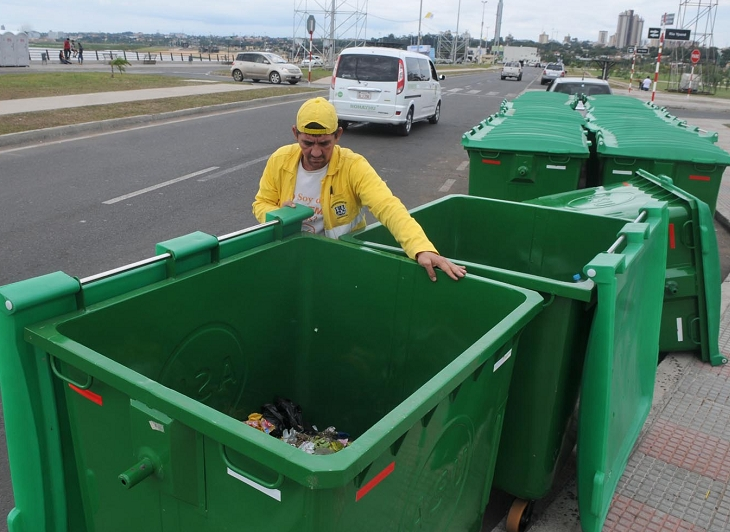
\includegraphics[width=7cm]{contenedores_mda.png}
    \caption{Contenedores de la ciudad de Asunción. [Fuente: Diario Última Hora (2015)]}
    \label{fig:contenedoresMDA}
\end{figure}

\subsection{Reciclaje de residuos sólidos}

El reciclaje es el resultado de una serie de actividades a través de las cuales, materiales que se tornarían residuos, son desviados, siendo recolectados, separados y procesados para ser usados como materia prima en la producción de un nuevo producto de composición semejante.

Entre los beneficios y ventajas del reciclaje se encuentran: la preservación de los recursos naturales, menor contaminación, ahorro de energía, dinero y petróleo, además, fomenta el consumo responsable y genera empleos.

\subsection{Administración pública y desarrollo sostenible}

La gestión de los residuos sólidos en el Paraguay, así como en la mayoría de los demás países, recae en el fuero municipal, se debe contar con políticas y estrategias nacionales para el desarrollo sostenible de la misma. La ausencia de planificación e infraestructura inadecuada para la eliminación de residuos sólidos conduce a una gran cantidad de residuos que se descargan en áreas públicas sin preparación del suelo, como vertederos a cielo abierto y ríos.

\subsection{Métodos de previsión y planificación}

El proceso de desarrollo urbano conlleva el crecimiento poblacional, cambios en patrones de consumo e incremento en el ingreso, siendo éstos, los principales factores que explican el aumento en la generación de residuos sólidos domiciliarios \citep{Vasquez2005ModeloChile}. Es por ello que es importante la elaboración de planes relacionados a la reducción de residuos sólidos, y la implementación de técnicas de previsión y modelos para predecir la generación de residuos, aumentando de esta manera la vida útil de los rellenos sanitarios en cuanto a su capacidad operativa o planes de expansión de instalaciones (tratamiento, traslado, y disposición).

\subsection{Determinación de sitios de disposición de residuos}

La selección de sitios para la disposición de residuos es un proceso complejo y considera criterios relacionados con el medio ambiente (suelo, características, declinación de la tierra, agua subterránea, ecosistema y geología), económico (presencia de caminos, distancia de las áreas residenciales, acceso al sitio y distancia de los centros de generación de residuos), y perspectivas sociales (aceptación de la población, proximidad a aeropuertos y sitios arqueológicos) \citep{Gbanie2013ModellingLeone}. Los métodos indiscriminados de eliminación de residuos han provocado la contaminación de cuerpos de agua, suelo y aire, lo que presenta importantes riesgos para la salud pública.

\section{Gestión de residuos sólidos urbanos en la ciudad de Asunción}

El área de estudio es Asunción, capital y ciudad más poblada de la República del Paraguay (según las proyecciones de \citet{2015Proyeccion2000-2025} para el año 2019 se estima una población aproximada de 522.287 habitantes). Es un municipio autónomo administrado como Distrito capital, cuenta con una superficie de 117 km$^{2}$. El ingreso promedio de personas en ómnibus del transporte público y vehículos privados de los municipios aledaños es alrededor de 1.320.000 diariamente. Este análisis se hace en base a cálculos estimativos de la Unidad Coordinadora del Programa Metrobús del Ministerio de Obras Públicas y Comunicaciones (MOPC) \citep{DiarioABCColor2016PorColor}. La cantidad de personas que convergen diariamente en Asunción trae consigo una alta generación de residuos, y esto hace que la complejidad en la gestión sea cada vez mayor.

Para el desarrollo de esta investigación se trabaja estrechamente con la DSU de la MDA, entidad encargada de la regulación y prestación de servicios de aseo, recolección, disposición y tratamiento de los residuos del municipio, así como también del equipamiento, mantenimiento, limpieza y ornato de la infraestructura pública del municipio, incluyendo las calles, avenidas, parques, plazas, balnearios y demás lugares públicos.

% Según Rodrigo Velázquez, director de la DSU, el promedio diario normal de basura recogida suele ser entre 800.000 y 900.000 kilos \citep{LaNacion2016AsuncionBasura} [Dato obtenido en 9 de Enero de 2016]. 

En la actualidad, el Departamento de Recolección de la DSU es responsable de la recolección de residuos sólidos urbanos y divide la ciudad en 134 zonas para realizar la labor. Como mínimo, debe existir una calle empedrada para que los vehículos recolectores recojan los residuos, éste es el motivo por el que lugares marginales como los barrios denominados ``Bañados Norte y Sur'' no son beneficiados con el servicio.

% El municipio cuenta con contenedores distribuidos por el microcentro capitalino, estos son recogidos de la misma manera que los residuos domiciliarios.

\subsection{Procedimiento de recolección de residuos urbanos en la Municipalidad de Asunción}

% A continuación se detalla el procedimiento llevado a cabo habitualmente para la recolección de los residuos domiciliarios:
A continuación se detalla el procedimiento que se lleva a cabo habitualmente para la recolección de los residuos domiciliarios:

\begin{enumerate}
% \item Se establecen los días y frecuencias de recolección para cada zona.
\item Un equipo de trabajo que cuenta con un chofer y tres recolectores es asignado a un vehículo y una zona. El vehículo es identificado por su chapa o por el número de identificación del camión proveído por la DSU.
\item Se realiza una recogida no selectiva.
\item El vehículo recolector inicia su recorrido cuando parte de la DSU en dirección a su zona. Antes de partir se controla el nivel de combustible y de acuerdo a esto se procede a la carga del mismo, en caso de que fuese necesario. Se entrega al chofer una orden de trabajo del día con la hora de salida. En la Figura \ref{fig:vehiculoRecolectorMDA}, se muestran vehículos recolectores de la MDA.

\begin{figure}[H]
    \centering
    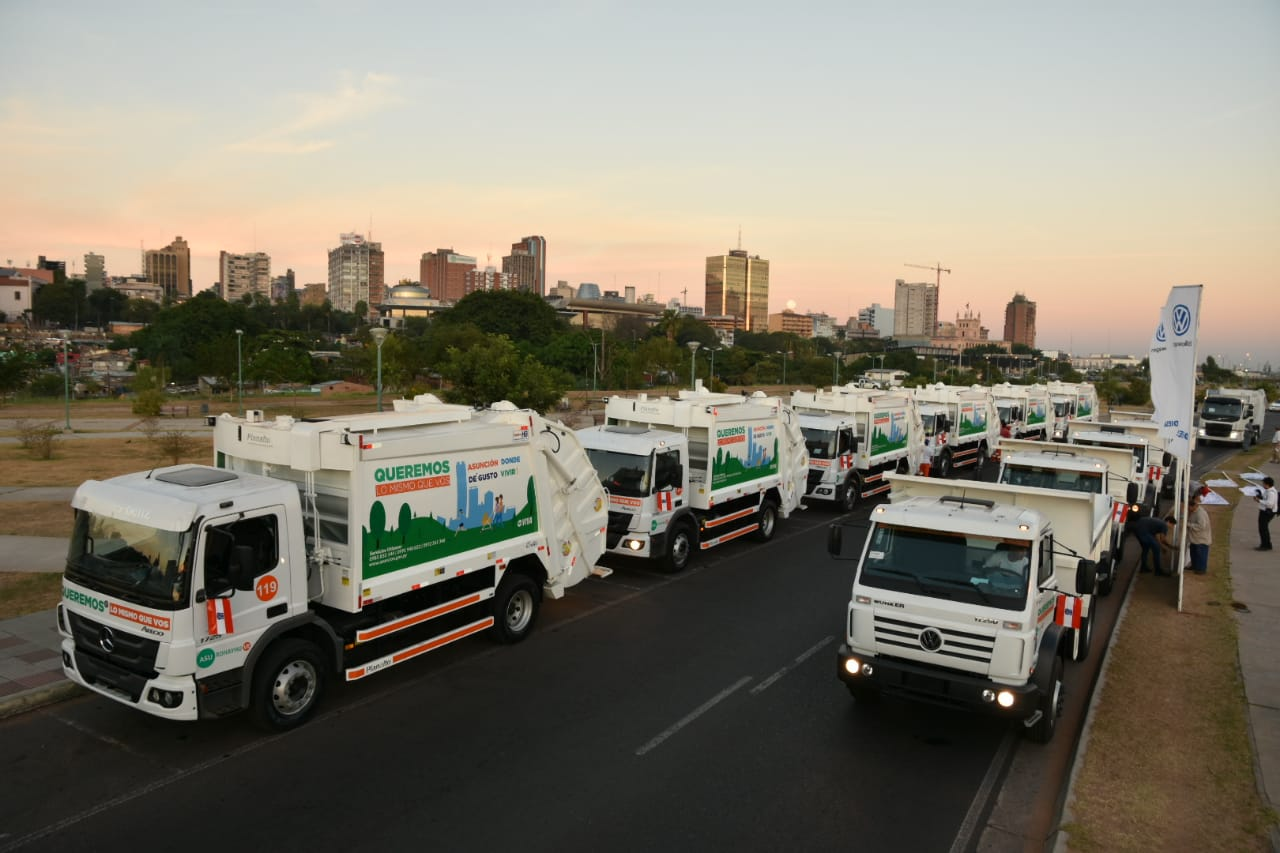
\includegraphics[width=7cm]{camion_recolector_mda.png}
    \caption{Vehículos recolectores de la MDA. [Fuente: MDA(2018)]}
    \label{fig:vehiculoRecolectorMDA}
\end{figure}

\item Luego de haber recogido toda la basura domiciliaria de la zona, el vehículo se dirige al relleno sanitario Cateura para depositar los residuos. 
\item Una vez que el chofer llega a Cateura, el camión pasa por un pesaje por ejes con báscula y el chofer entrega la orden de trabajo a un fiscalizador que se encuentra en el puesto de pesaje. Un grupo de personas de seguridad se encargan de coordinar la entrada y salida de vehículos, así como de guiar la descarga de lo recolectado. 
\item Una vez que se vacía el vehículo, uno de los encargados guía nuevamente al chofer hacia la salida, en donde el vehículo es pesado de vuelta, calculando el peso de lo recolectado resultado de la diferencia del peso de entrada y salida, que se detalla en la orden de trabajo la cual es devuelta al chofer. En la orden de trabajo también se especifican la hora de entrada y salida del vehículo al relleno sanitario.
\item El equipo vuelve al punto de partida una vez vaciado el vehículo recolector y el chofer entrega la orden de trabajo al Departamento de Recolección.  
\end{enumerate}

Generalmente, el vehículo tiene capacidad suficiente para realizar un solo viaje de su zona a Cateura, pero si no es el caso, debe realizar la cantidad de viajes necesarios hasta recolectar todos los residuos domiciliarios de la zona en cuestión. La carga máxima admitida de un vehículo recolector en circulación por el Departamento de Recolección de la DSU es de 8500 kilogramos (kg). En caso de que el equipo de trabajo estime, en base a su experiencia, que la cantidad total a recoger de la zona será mayor a la permitida, entonces realizará más de un viaje a Cateura.

La segregación de los residuos no forma parte del proceso llevado a cabo por la DSU, es por ello que en Cateura se encuentran trabajando los gancheros, personas dedicadas a recuperar, separar o reducir, de los residuos sólidos urbanos, aquellos que posean valor comercial para su reutilización o reciclaje.

El servicio de recolección domiciliaria se realiza de lunes a sábados, y se divide en tres turnos: mañana, tarde y noche; donde cada turno tiene una duración máxima de 6 horas debido al carácter insalubre de las tareas realizadas por el personal encargado de brindar el servicio.

En la Figura \ref{fig:zonasRecoleccion} se muestran las zonas de recolección de basura de Asunción. Las zonas pintadas en celeste corresponden al microcentro de Asunción y tienen un tratamiento diferente a las demás, ya que son las únicas que son atendidas de lunes a viernes y sus residuos son recolectados en el turno noche debido al poco tráfico registrado en esas calles en comparación a cualquier otro turno. De igual manera, las avenidas más importantes de la ciudad también son recolectadas en el turno noche de lunes a viernes. Las demás zonas reciben el servicio cada dos días, tres veces por semana.

\begin{figure}[H]
    \centering
    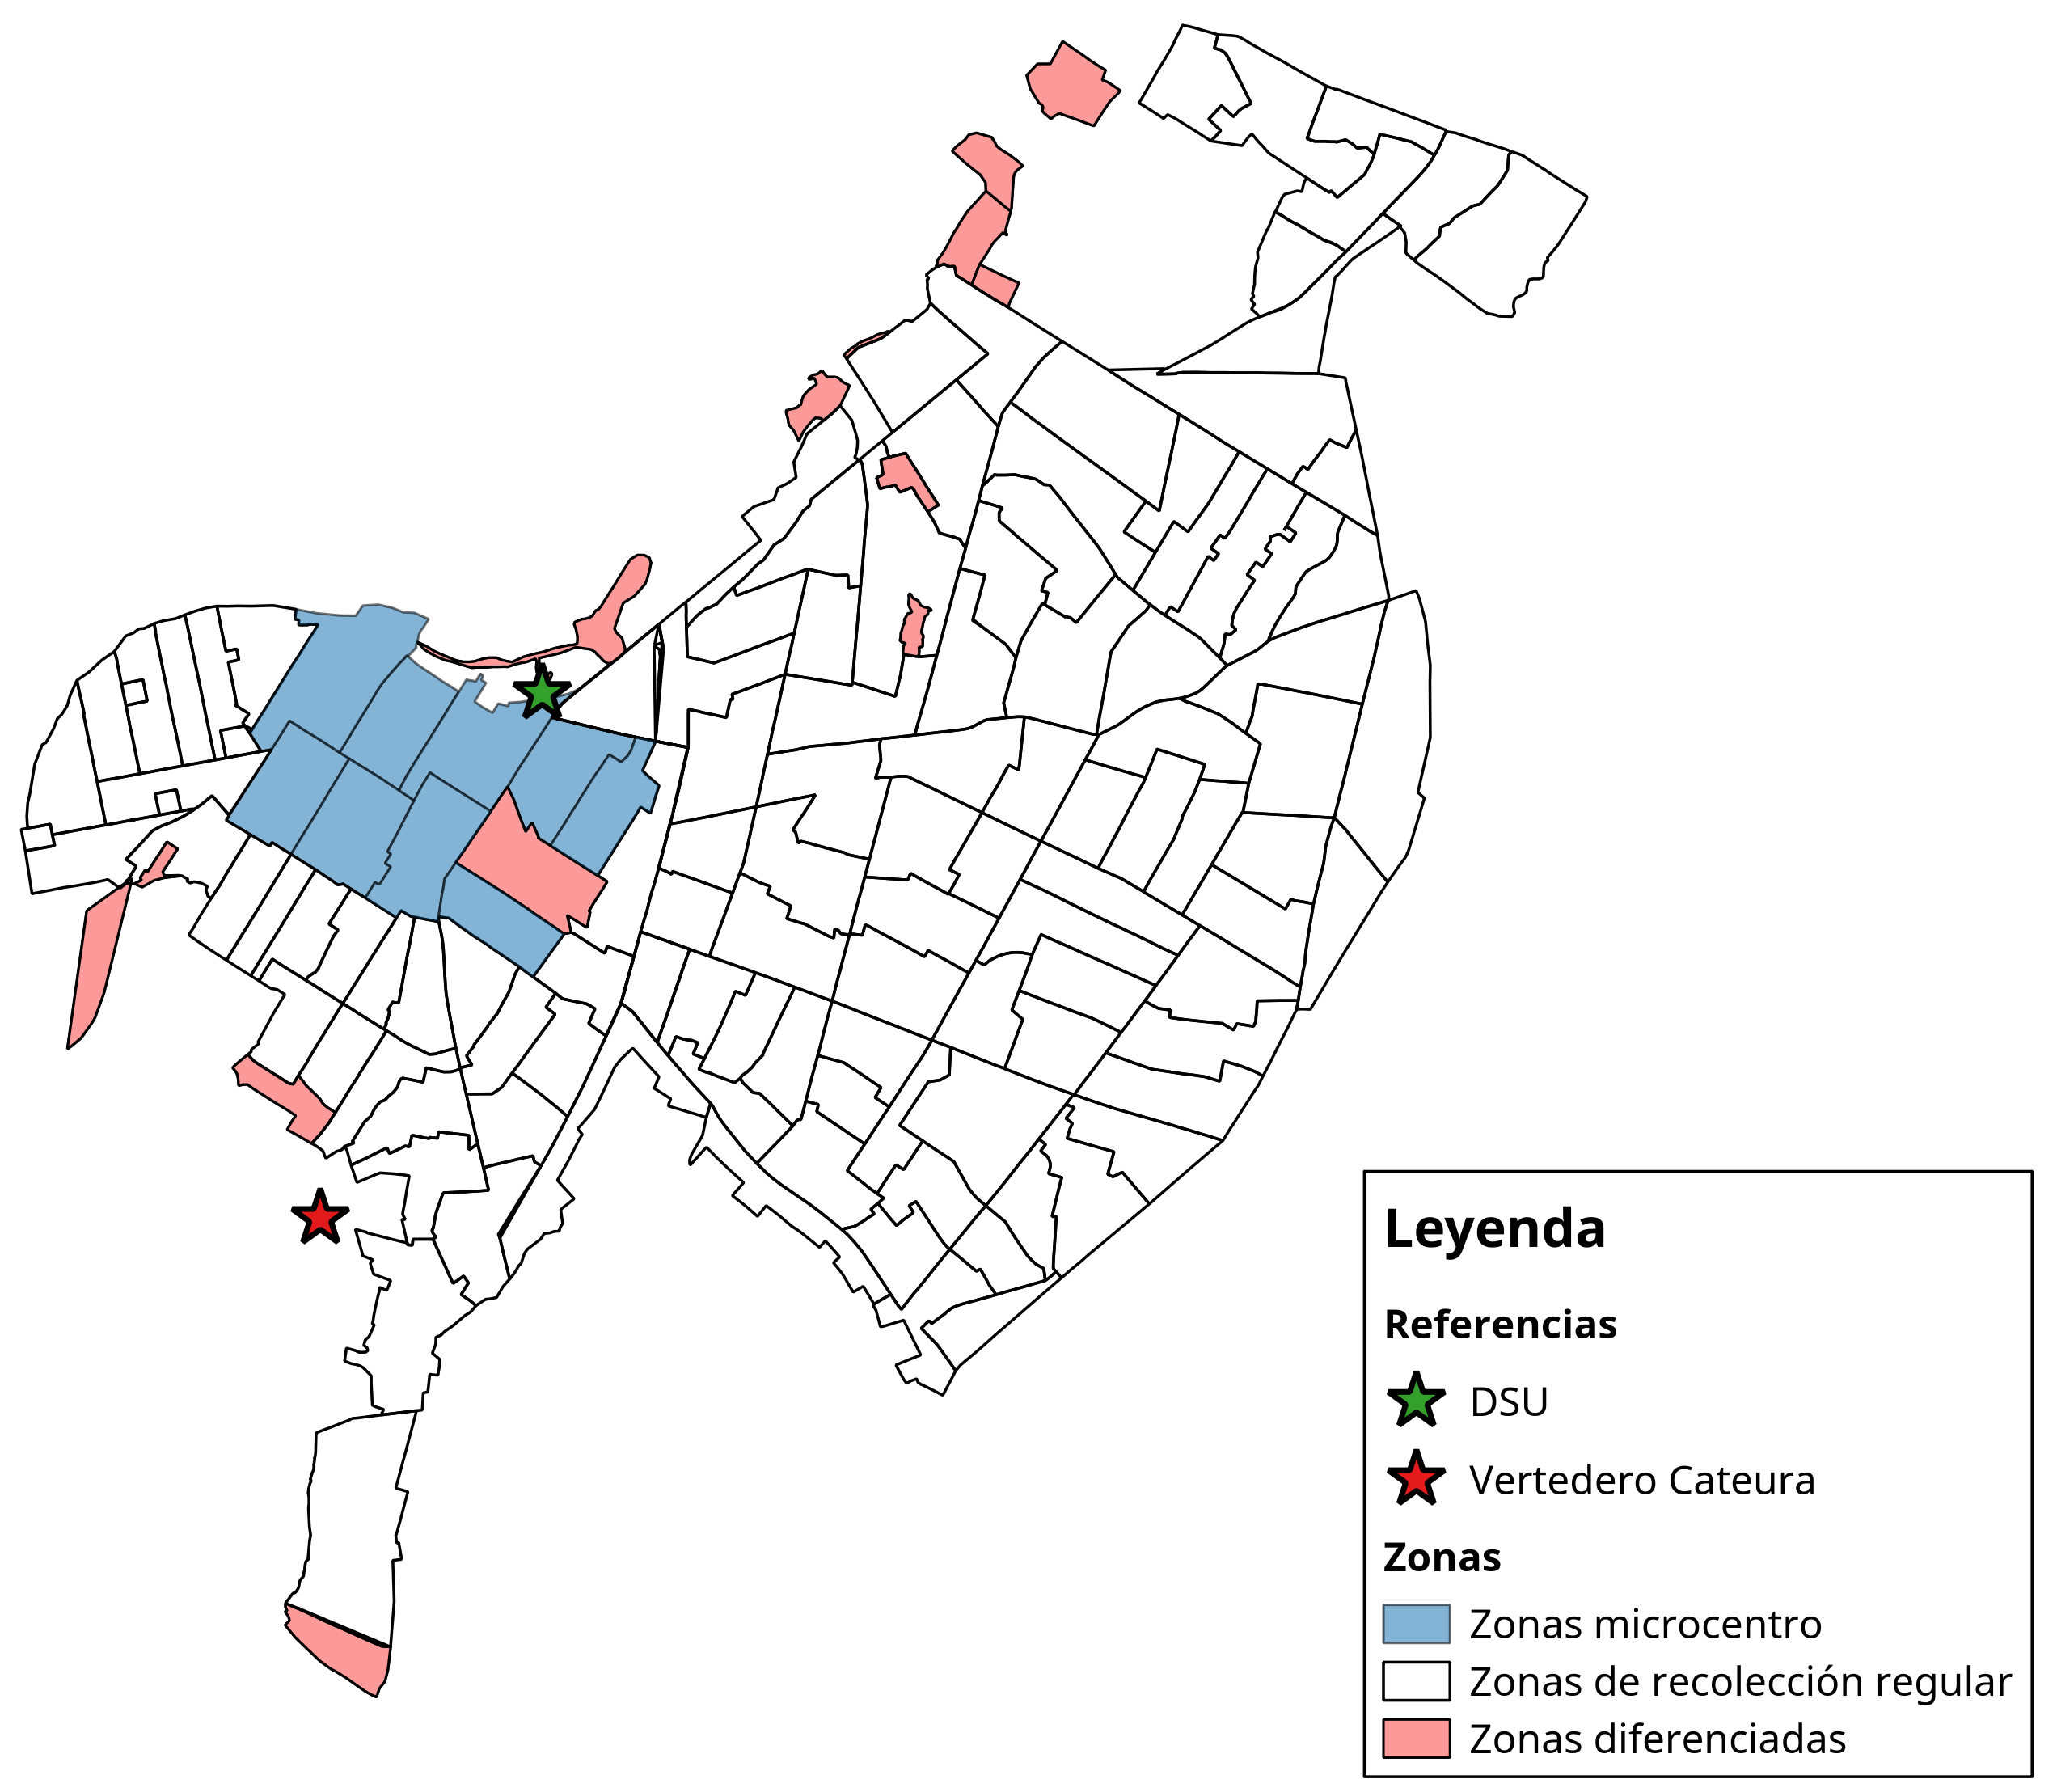
\includegraphics[width=8cm]{Recoleccion-ZONAS_CUADRANTES.png}
    \caption{División de la ciudad en zonas.}
    \label{fig:zonasRecoleccion}
\end{figure}

Los residuos sólidos de grandes generadores son todos aquellos residuos sólidos urbanos comerciales cuyas cantidades requieran una recolección diferenciada, esta recolección no forma parte del procedimiento descrito más arriba y tampoco se incluye en el alcance de este trabajo. Los residuos hospitalarios son recolectados por una empresa tercerizada por el municipio y no son depositados en Cateura.

% En la actualidad, los choferes de los vehículos recolectores de basura de la ciudad de Asunción trazan los caminos a seguir en base a su experiencia, razón por la cual es necesario optimizar el recorrido realizado para la recolección de residuos, reduciendo el costo y el tiempo de cada recorrido. Se propone desarrollar una aplicación que permita gestionar de manera eficiente esos recorridos al poder actualizar el sentido de las calles, inhabilitar calles, agregar restricciones de giro o de continuar el sentido (contramano).

% \begin{itemize}
% \item Se establecen los días y frecuencias de recolección para cada zona.
% \item Un equipo de trabajo cuenta con un chofer y tres recolectores, que es asignado a un vehículo y una zona. El vehículo es identificado por su chapa o por el número de identificación del camión proveído por la DSU. Estos vehículos recolectores son de propiedad de la MDA, en caso de que uno de ellos quede fuera de servicio por algún desperfecto, por lo general, la solución radica en alquilar un recolector para que lo cubra. TODO: la ultima oracion es la que se quito del paper
% \item Se realiza una recogida no selectiva. En la Ordenanza Municipal N$^{\circ}$ 408/14 se establece que los usuarios del servicio ordinario de recolección deberán almacenar sus residuos en el interior de las viviendas o locales correspondientes, en  sitios adecuados, en bolsas perfectamente cerradas, las cuales serán sacadas y colocadas en la acera, solamente en los días señalados, momento antes del horario fijado para el servicio. No se permitirá el acopio o acumulación de los residuos en la vía pública, ya sea directamente sobre las aceras o en canastos elevados en días y horas distintos a los establecidos para el servicio de recolección. TODO: la parte de la ordenanza es la que se omitio en el paper
% \item El vehículo recolector inicia su recorrido cuando parte de la DSU en dirección a su zona. Antes de partir se controla el nivel de combustible y de acuerdo a esto se procede a la carga del mismo, en caso de que fuese necesario. Se entrega al chofer una orden de trabajo del día con la hora de salida. En la Figura \ref{fig:vehiculoRecolectorMDA}, se muestra un vehículo recolector de la MDA.
% \item Luego de haber recogido toda la basura domiciliaria de la zona, el vehículo se dirige al relleno sanitario Cateura para depositar los residuos y de allí vuelve a su punto de partida. Generalmente, el vehículo tiene capacidad suficiente para realizar un solo viaje de su zona a Cateura, pero si no es el caso, debe realizar la cantidad de viajes necesarios hasta recolectar todos los residuos domiciliarios de la zona en cuestión. La carga máxima admitida de un vehículo recolector en circulación por el Departamento de Recolección de la DSU es de 8500 Kg, en caso de que el equipo de trabajo estime, en base a su experiencia, que la cantidad total a recoger de la zona será mayor al permitido, entonces realiza más de un viaje a Cateura.
% \item Una vez que el chofer llega a Cateura, el camión pasa por un pesaje por ejes con báscula y el chofer entrega la orden de trabajo a un fiscalizador que se encuentra en el puesto de pesaje. Un grupo de personas de seguridad se encargan de coordinar la entrada y salida de vehículos, así como de guiar la descarga de lo recolectado. En el lugar se encuentran varios gancheros que ayudan a sacar los residuos del vehículo, los gancheros son personas dedicadas a recuperar, separar o reducir, de los residuos sólidos urbanos, aquellos que posean valor comercial para su reutilización o reciclaje. Una vez que se vacía el vehículo, uno de los encargados guía nuevamente al chofer hacia la salida, en donde el vehículo es pesado de vuelta, calculando así el peso de lo recolectado, que se detalla en la orden de trabajo la cual es devuelta al chofer. En la orden de trabajo también se especifican la hora de entrada y salida del vehículo al relleno sanitario.
% \item Una vez que el equipo de trabajo se encuentra de vuelta en la DSU, el chofer entrega la orden de trabajo al Departamento de Recolección.
% \end{itemize}

%TODO: cambiar por el shape que nos dieron%


% El servicio de recolección domiciliaria se realiza de lunes a sábados, y se divide en tres turnos: mañana, tarde y noche; donde cada turno tiene una duración máxima de 6 horas debido al carácter insalubre de las tareas realizadas por el personal encargado de brindar el servicio.

% En la figura \ref{fig:zonasRecoleccion} un turno se corresponde con un conjunto de zonas, las zonas pintadas en azul oscuro, correspondientes al microcentro de Asunción, tienen un tratamiento diferente a las demás zonas, ya que son las únicas que son atendidas de lunes a viernes, las demás zonas reciben el servicio cada dos días, tres veces por semana. Los residuos en estas zonas son recolectados en el turno noche debido al poco tráfico registrado en esas calles en comparación a cualquier otro turno, de igual manera, las avenidas más importantes de la ciudad también son recolectadas en el turno noche de lunes a viernes, los equipos de trabajo que recogen los residuos a lo largo de estas avenidas les corresponden dos avenidas por noche. Las zonas no pintadas no tienen número, y por ende no son cubiertas por el servicio, sin embargo representan una zona candidata a futuro para la recolección de la basura.

% Los residuos sólidos de grandes generadores son todos aquellos residuos sólidos urbanos comerciales cuyas cantidades requieran una recolección diferenciada, esta recolección no forma parte del procedimiento descrito más arriba y tampoco se incluye en el alcance de este trabajo. Los residuos hospitalarios son recolectados por una empresa tercerizada por el municipio y no son depositados en Cateura.

% La recolección de los residuos de manejo especial y peligrosos no forman parte lo descrito más arriba y tampoco forman parte del alcance de este trabajo. % Mejora de imagen 

\clearpage
\lhead{\emph{Sistemas de Información Geográfica}} 
\renewcommand\chaptername{Capítulo}%título "Capítulo"
\chapter{Sistemas de Información Geográfica}
\label{chap3}
\ifpdf
    \graphicspath{{Chapter3/Chapter3Figs/PNG/}{Chapter3/Chapter3Figs/PDF/}{Chapter3/Chapter3Figs/}}
\else
    \graphicspath{{Chapter3/Chapter3Figs/EPS/}{Chapter3/Chapter3Figs/}}
\fi

\markboth{\hfill \thechapter. Sistemas de Información Geográfica}{\hfill \thechapter. Sistemas de Información Geográfica}

Los SIG o GIS han sido definidos por varios especialistas y estudiosos. De acuerdo con \citet{Burrough1986PrinciplesAssessment} un SIG es “un conjunto de herramientas para recopilar, almacenar, recuperar a voluntad, transformar y visualizar datos espaciales del mundo real para un conjunto particular de propósitos”. \citet{NCGIA1990IntroductionGIS} lo define como “un sistema de hardware, software y procedimientos diseñado para realizar la captura, almacenamiento, manipulación, análisis, modelización y presentación de datos referenciados espacialmente para la resolución de problemas complejos de planificación y gestión”.

El SIG es una herramienta que favorece el análisis de la información espacial, es por ello que existen miles de trabajos que lo han utilizado y aprovechado. \citet{Cabral2018EstrategiasAsuncion} plantearon una estrategia de planificación que contribuya al mejoramiento del manejo integrado de los RSU con servicios diferenciales mediante tecnología SIG aplicada a la cuenca del Arroyo Ferreira en Asunción. \citet{Acosta2006LevantamientoCaballero} realizaron un levantamiento topográfico y SIG para el abastecimiento de energía eléctrica por vía subterránea línea de 220 kV: tramo Estación Puerto Botánico a Parque Caballero.

% Por ejemplo, \citet{OsorioDominguez2018AnalisisParaguay} realizaron un análisis multitemporal de la pérdida del hábitat y distribución espacial del mono capuchino (sapajus cay) en la ecorregión selva central, Paraguay.

Ya que el número de terminologías en torno a estos sistemas es muy grande, en este capítulo se explicarán los conceptos básicos que servirán de apoyo para una clara interpretación de los siguientes capítulos donde han sido aplicados.

\section{Origen de los datos espaciales}

Hoy en día, los datos que son recolectados en censos, encuestas o sistemas informáticos van acompañados de coordenadas de ubicación. Estas informaciones pueden provenir de dispositivos especializados, teléfonos móviles, tabletas o cámaras. En otras ocasiones, pueden ser generadas de forma manual a través de operaciones o dibujándolas directamente en sistemas SIG, CAD (\textit{Computer-Aided Design}) u otros sistemas capacitados para ello.

Resulta muy común, en la actualidad, que dispositivos electrónicos tengan incorporado internamente un receptor GPS. El Sistema de Posicionamiento Global (GPS, \textit{Global Positioning System}) es un sistema que permite determinar la posición de un objeto en la Tierra (Ver Figura \ref{fig:gps}). Así también, existen otros mecanismos de geolocalización como por ejemplo: las redes inalámbricas, bluetooth, identificación por radiofrecuencia (RFID, \textit{Radio Frequency Identification}), entre otros.

\begin{figure}[H]
    \centering
    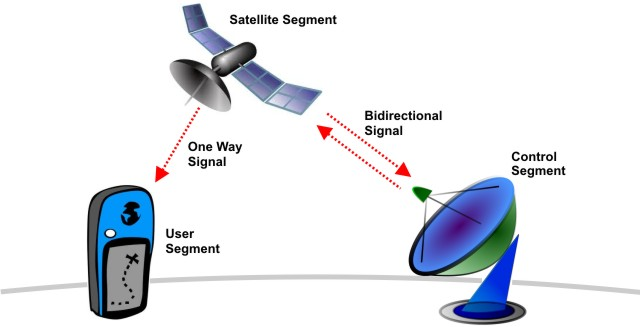
\includegraphics[width=11.5cm]{gps.jpg}
    \caption{Ilustración de los tres principales componentes del GPS. [Fuente: \citet{Hinch2010OutdoorGps}]}
    \label{fig:gps}
\end{figure}

Otra fuente principal de extracción de datos geográficos provienen de las imágenes orto-rectificadas. Las imágenes orto-rectificadas son el resultado del tratamiento de un conjunto de fotografías tanto de satélite como aéreas, donde son corregidas para representar una proyección ortogonal sin efectos de perspectiva, y en la que, por lo tanto, es posible realizar mediciones exactas. Esta fuente es una de las más utilizadas para generar nuevos datos geográficos.

Toda la información en un SIG está vinculada a una referencia espacial, podemos hablar entonces de dos tipos de informaciones: 
\begin{itemize}
    \item \textbf{La información de ubicación:} 
    Describe la posición de las características geográficas particulares en la superficie de la Tierra.
    \item \textbf{La información de atributos:} 
    Describe propiedades de las características geográficas representadas, como su nombre o número, información cuantitativa como su área o longitud, y cualquier otra información asociada a la entidad.
\end{itemize}

Para presentar los datos espaciales, la forma más común es a través de un mapa. Según la Asociación Cartográfica Internacional, un mapa ``es una representación, normalmente a escala y en un medio plano, de una selección de características materiales o abstractas en, o en relación con, la superficie de la Tierra". La escala de un mapa indica la relación de distancia sobre el mapa y su distancia correspondiente sobre la superficie terrestre en la realidad.

La Figura \ref{fig:capasGis} muestra como en los SIG los mapas están organizados lógicamente en un conjunto de capas o temas de información. Un mapa base puede organizarse en capas tales como: carreteras, suelos, límites de estados, ciudades.

\begin{figure}[H]
    \centering
    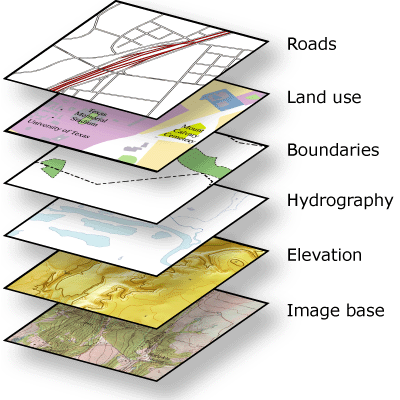
\includegraphics[width=7cm]{capas_gis.png}
    \caption{Organización de capas. [Fuente: arcgis.com]}
    \label{fig:capasGis}
\end{figure}

\section{Referencia espacial}

Los investigadores han confirmado que la superficie de la Tierra no es esférica ni plana sino que es oblata elipsoidal, lo que significa que todos los puntos de la superficie terrestre no son equidistantes del centro geométrico. Para localizar y poder representar los elementos existentes sobre la Tierra en un SIG, existe la necesidad de contar con sistemas de referencia de coordenadas (SRC, en inglés CRS; \textit{Coordinate Reference System}). Los Datums definen los sistemas de referencia que describen el tamaño y la forma de la Tierra, y el origen y la orientación de los sistemas de coordenadas utilizados para mapear la Tierra.

Los tipos de Datums se clasifican en:
\begin{itemize}
    \item \textbf{Horizontal:} 
    Datums que definen la relación entre la Tierra y las coordenadas horizontales. En otras palabras, describe un punto sobre la superficie terrestre, como la latitud y la longitud.
    \item \textbf{Vertical:} 
    Datums que definen superficies de nivel, midiendo elevaciones o profundidades. Algunos se basan en mediciones del nivel del mar y redes de nivelación, otros en mediciones de la gravedad.
    \item \textbf{Completo:} 
    Datums que describen los sistemas verticales y horizontales. Algunos, como el \textit{World Geodetic System 1984} (WGS84), también describen otros parámetros, como la velocidad de rotación de la Tierra y diversas constantes físicas, como la velocidad angular y la constante gravitacional de la Tierra.
\end{itemize}

Por otro lado, los sistemas de referencia espacial se agrupan principalmente en: Sistemas de coordenadas geográficas y Sistemas de coordenadas rectangulares (también denominados como: proyectados, planos o cartesianos); los cuáles los detallaremos a continuación.

\subsection{Sistema de coordenadas geográficas}
Los sistemas de coordenadas geográficas se componen de la latitud y la longitud. Las líneas de longitud (también conocidas como meridianos) comienzan en un polo y se propagan hacia afuera hasta que convergen en el polo opuesto. Las líneas de latitud (también conocidas como paralelos) se encuentran en ángulo recto a las líneas de longitud y corren paralelas entre sí (Ver Figura \ref{fig:latitudLongitud}). 

\begin{figure}[H]
    \centering
    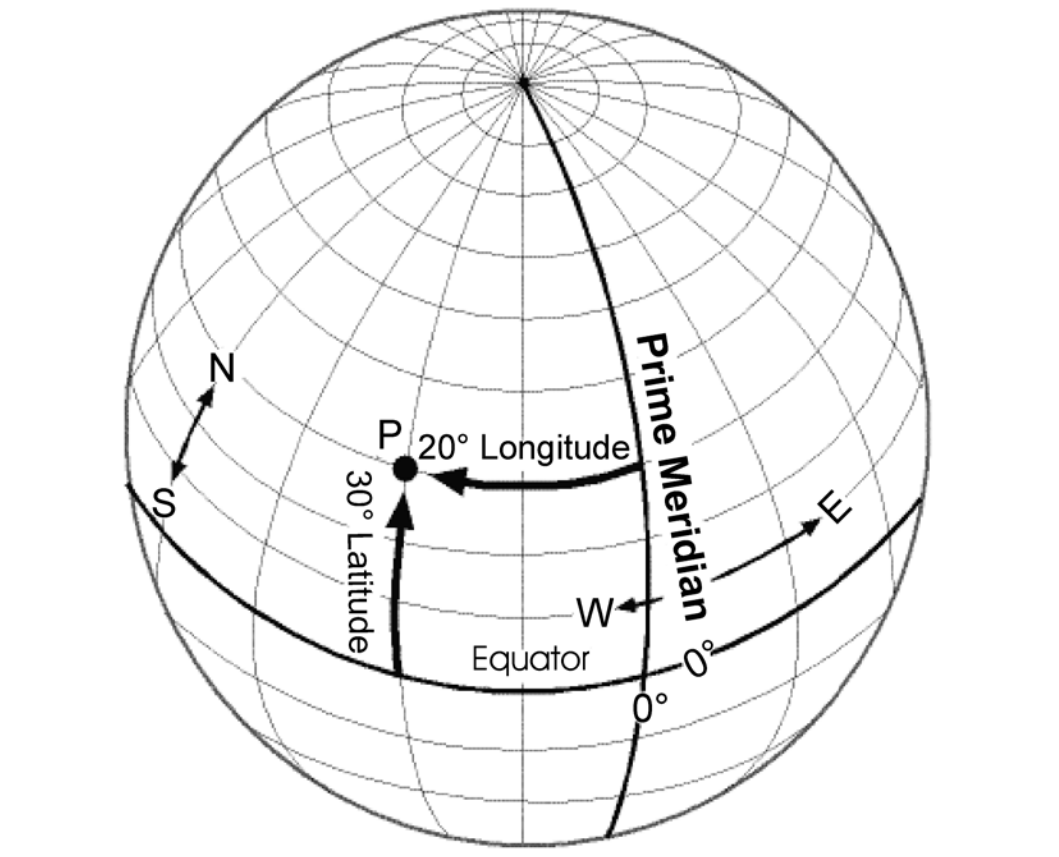
\includegraphics[width=10cm]{CoordenadasGeograficas.png}
    \caption{Representación de coordenadas geográficas. [Fuente: \citet{Fazal2008GISBasics}]}
    \label{fig:latitudLongitud}
\end{figure}

La elección arbitraria de una línea central de longitud corresponde a la que atraviesa el Observatorio Real en Greenwich, Inglaterra; se conoce como el meridiano de Greenwich o el meridiano principal, y las longitudes
al este u oeste se especifican como ángulos de giro con respecto al meridiano de Greenwich, variando de -180\grad (oeste) a 180\grad (este). La latitud es la distancia angular entre la línea ecuatorial (el ecuador), y un punto determinado de la Tierra, y las latitudes al sur y al norte varían en un rango de hasta 90\grad.

Las coordenadas geográficas son expresadas, por lo general, en grados, minutos y segundos, pero para su uso en los SIG son transformadas en grados decimales. Algunos ejemplos de las formas de representar las coordenadas ubicadas en un punto dentro de Asunción se muestran en la Tabla \ref{table:coordenadasGeograficas}.

\begin{table}[H]
\caption{Representación de coordenadas geográficas (WGS84).}
\centering
\begin{tabular}{cccc}
\hline
\multirow{2}{*}{Coordenadas} & \multirow{2}{*}{Grados, minutos y segundos} & \multicolumn{2}{c}{Grados decimales} \\ \cline{3-4} 
                             &                                             & Sin signo          & Con signo       \\ \hline
Latitud                      & 25\grad 16' 54.84'' Sur                            & 25.2819 Sur        & -25.2819        \\
Longitud                     & 57\grad 38' 6'' Oeste                                & 57.635 Oeste       & -57.635         \\ \hline
\end{tabular}
\label{table:coordenadasGeograficas}
\end{table}

\subsection{Sistema de coordenadas rectangulares}
Las proyecciones sirven para representar sobre un plano la superficie esférica de la Tierra con la menor deformación posible. El proceso de transferencia de la Tierra esférica a una superficie bidimensional, definidos normalmente mediante dos ejes perpendiculares \textit{XY} y en el caso de sistemas tridimensionales añadiendo un eje \textit{Z} perpendicular a ambos, introduce errores en los datos espaciales cuyo carácter variará dependiendo del método de proyección elegido. 

% Algunas proyecciones harán que la distancia entre las entidades espaciales se mantenga mientras la dirección está distorsionada. En otros casos, la forma puede conservarse a expensas de estimaciones de área precisas.

Podemos agruparlas en tres sistemas básicos según el tipo de plano auxiliar utilizado para proyectar la superficie terrestre: cilíndrica, cónica y acimutal (Ver Figura \ref{fig:capasGis}).

\begin{figure}[H]
    \centering
    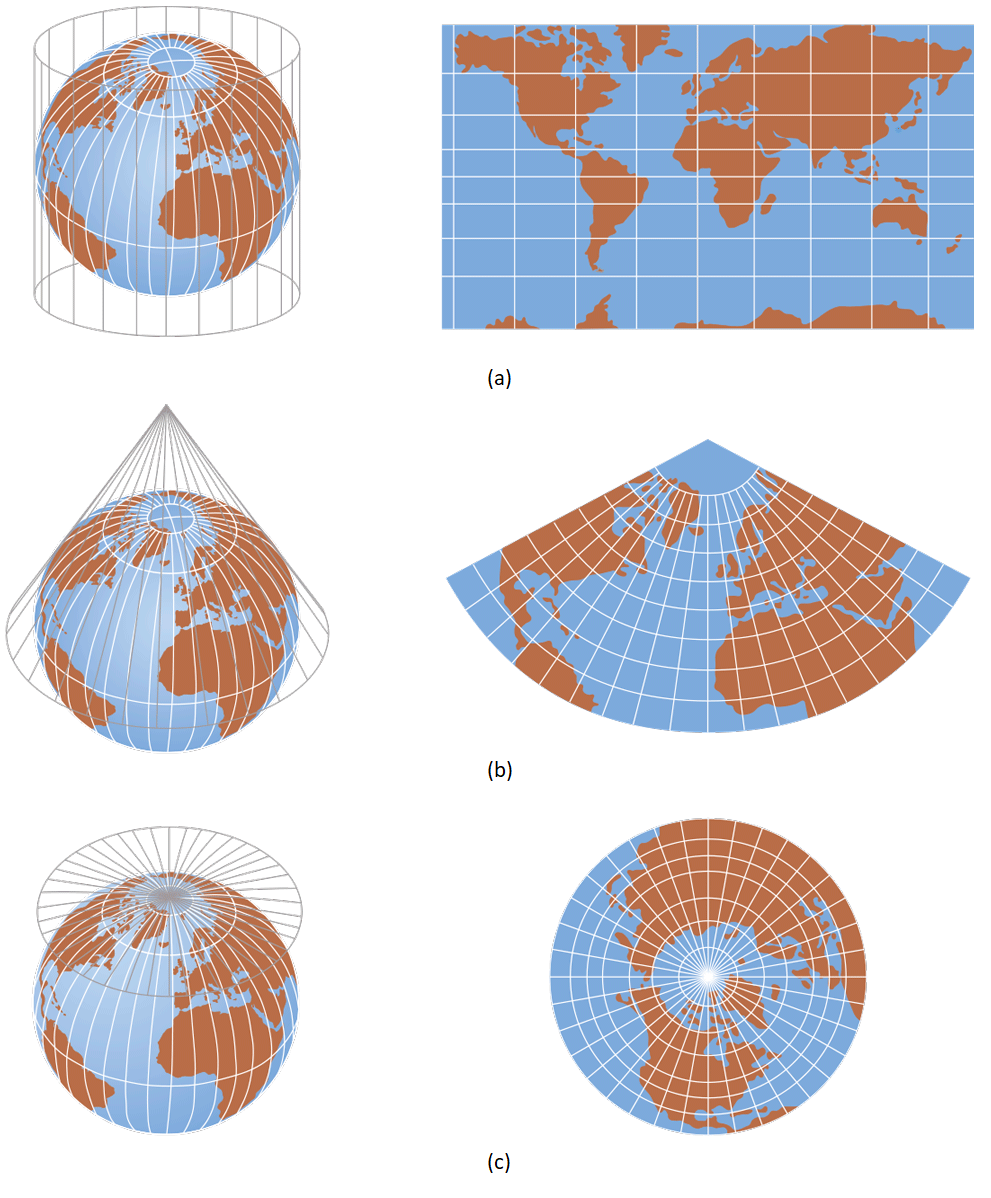
\includegraphics[width=10cm]{Chapter3/Chapter3Figs/CoordenadasProyectadas.png}
    \caption{Representación de tipos de proyecciones: (a) Cilíndrica (b) Cónica (c) Acimutal. [Fuente: blinklearning.com]}
    \label{fig:mapaCoordenadasGeograficas}
\end{figure}

Las proyecciones más sofisticadas permiten la preservación de representaciones precisas: de áreas, de distancias, de ángulos o de otras características; pero no todas ellas pueden conservarse en una misma proyección. De hecho, por lo general solo se puede mantener la  precisión de una sola característica y las demás se presentan distorsionadas con respecto a la realidad.

En Paraguay, cartógrafos y otros trabajadores en el área han adoptado el sistema de cuadrícula plana de \textit{Universal Transverse Mercator} (UTM), la cual corresponde a la proyección de tipo cilíndrica. Este sistema utiliza la proyección transversal de Mercator y divide la Tierra en 60 zonas verticales que tienen 6 grados de longitud, evitando los polos. El sistema se expresa en metros, facilitando así los cálculos de distancia y superficie.

En los SIG, los SRC están asociados a un identificador estándar único, denominados Identificador de Referencia Espacial (SRID, \textit{Spatial Reference System Identifier}), también son conocidos como códigos EPSG (\textit{European Petroleum Survey Group}) ya que existen varios SRID que han sido definidos por el EPSG. Como ejemplos tenemos el código EPSG 4326 que corresponde a WGS84 en coordenadas geográficas y el EPSG 32721 que es para la zona 21 Sur en coordenadas UTM, y así es como cada SRC tiene asociado un código único EPSG/SRID.

En la Tabla \ref{table:coordenadasPlanas} se muestran las coordenadas planas de la zona 21 Sur ó 21J de UTM/WGS84 que ubica un punto dentro de Asunción.

\begin{table}[H]
\caption{Representación de coordenadas planas (UTM).}
\centering
\begin{tabular}{cccc}
\hline
Coordenadas & UTM     & Zona & Hemisferio \\ \hline
X           & 436068  & 21 J & Sur        \\
Y           & 7203687 & 21 J & Sur        \\ \hline
\end{tabular}
\label{table:coordenadasPlanas}
\end{table}

% \subsection{Sistema sin coordenadas}
% Los sistemas sin coordenadas proporcionan referencias espaciales utilizando un código descriptivo en lugar de una coordenada. Los códigos postales ampliamente utilizados en todo el mundo son un ejemplo. Algunos códigos postales son totalmente numéricos, como los códigos postales estadounidenses, mientras que otros son alfanuméricos, como en el caso del código postal del Reino Unido.

% Ejemplo de código postal en el Reino Unido: E1 6PX.

\section{Representación de los datos}

Las características de un mapa digital requieren ser representadas, y para ello se utilizan unas simbologías denominadas entidades espaciales cuyos tipos básicos son: puntos, líneas y polígonos (Ver Figura \ref{fig:entidadesPuntoLineaPoligono}). Con estos tres tipos es posible de forma sencilla representar todos los fenómenos geográficos del mundo real a través de un mapa. Adicionalmente, hay otras entidades como las redes y superficies; que son extensiones de las líneas y áreas (o polígonos) respectivamente.

\begin{figure}[H]
    \centering
    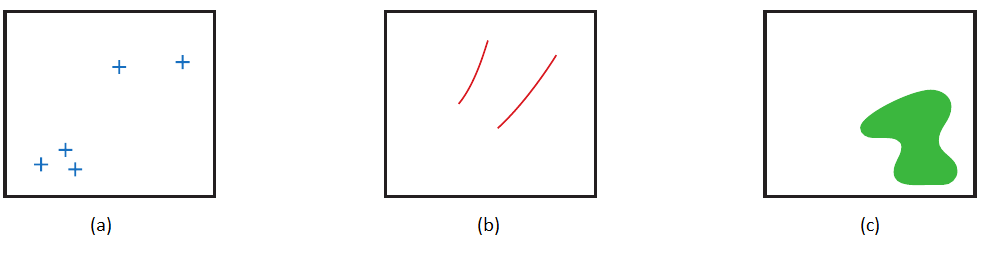
\includegraphics[width=10cm]{entidadesGeometricas.png}
    \caption{Entidades espaciales: (a) Puntos (b) Líneas (c) Áreas. [Fuente: \citet{Heywood2006AnSystems}]}
    \label{fig:entidadesPuntoLineaPoligono}
\end{figure}

Las características de un mapa a su vez pueden ser estructuradas mediante el uso de vectores y mediante el uso de matrices. Antes de detallar cada uno de estos sistemas, cabe mencionar que ambos se diferencian fundamentalmente en la estructura de los datos espaciales, en las relaciones topológicas, en el volumen físico de la información y en los métodos de análisis.

El concepto de Topología geoespacial es muy importante en los SIG y se lo define como ``el estudio de las relaciones espaciales entre las entidades espaciales y su posición en el mapa". Las relaciones topológicas, en relación a los datos, constan de tres elementos claves: adyacencia, contención y conectividad. En los sistemas matriciales las relaciones se producen entre celdas como análisis de vecindad generalmente; en los sistemas vectoriales se suelen basar en la relación arco-nodo que viene definida por la direccionalidad, la conectividad y la proximidad entre vectores.

\subsection{Sistema vectorial}

En el modelo vectorial, el punto es el bloque de construcción básico a partir del cual se construyen todas las entidades espaciales. El punto está representado por un único par de coordenadas (x,y). Las entidades de línea y área se construyen conectando una serie de puntos (Ver Figura \ref{fig:modeloVectorial}).

\begin{figure}[H]
    \centering
    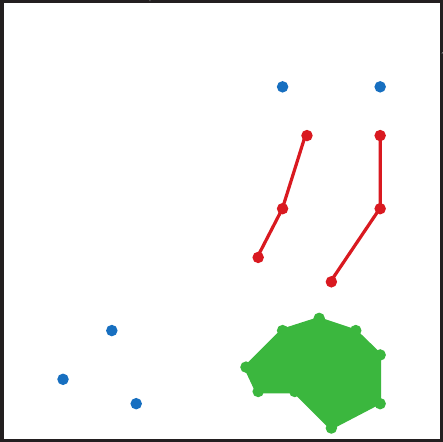
\includegraphics[width=7.5cm]{modeloVectorial.png}
    \caption{Representación de puntos, líneas y áreas en el sistema vectorial. [Fuente: \citet{Heywood2006AnSystems}]}
    \label{fig:modeloVectorial}
\end{figure}

Utilizando entidades de puntos se pueden representar cestos de basura residenciales, semáforos, árboles, alumbrados públicos. También a menor escala, es decir, en mapas más alejados y con menos detalle, puede utilizarse para indicar la ubicación de ciudades capitales. Las líneas se utilizan, mayormente, para representar calles, caminos, tendidos eléctricos, etc. Las áreas o polígonos corresponden a cuadras manzaneras, lotes, lagunas, países.

En el modelo vectorial, la representación de redes y superficies es una extensión del enfoque utilizado para almacenar entidades de línea y área respectivamente. Sin embargo, el método es más complejo y está estrechamente relacionado con la forma en que se estructuran los datos para la codificación por computadora.

Las líneas de contorno y las redes irregulares de triángulos (TIN; \textit{Triangulated Irregular Network}) se utilizan para representar la altitud u otros valores en continua evolución. Los TIN son registros de valores en un punto localizado, que están conectados por líneas para formar una malla irregular de triángulos. La cara de los triángulos representan, por ejemplo, la superficie del terreno.

\subsection{Sistema ráster}

En un sistema ráster se ubica una cuadrícula imaginaria sobre el mapa. Cada celda de la cuadrícula, conocida como elemento de imagen o píxel, se examina para ver qué característica cae dentro de ella. El resultado final de este proceso es una cuadrícula o una serie de cuadrículas de números que representan las características en el mapa. (Ver Figura \ref{fig:modeloRaster}).

\begin{figure}[H]
    \centering
    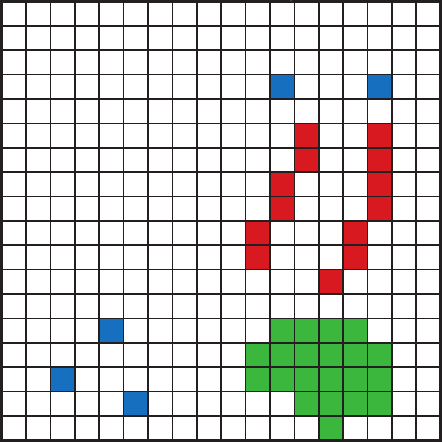
\includegraphics[width=7.5cm]{modeloRaster.png}
    \caption{Representación de puntos, líneas y áreas en el sistema ráster. [Fuente: \citet{Heywood2006AnSystems}]}
    \label{fig:modeloRaster}
\end{figure}

Este modelo se centra en las propiedades del espacio más que en la precisión de la localización. Divide el espacio en celdas regulares donde cada una de ellas representa un único valor. Se trata de un modelo de datos muy adecuado para la representación de variables continuas en el espacio. El tamaño de la celda de la cuadrícula es muy importante ya que influye en cómo aparece una entidad. En la Figura \ref{fig:rasterResolution} se muestra que cuanto mayores sean las dimensiones de las celdas menor es la precisión o detalle (resolución) de la representación del espacio geográfico.

\begin{figure}[H]
    \centering
    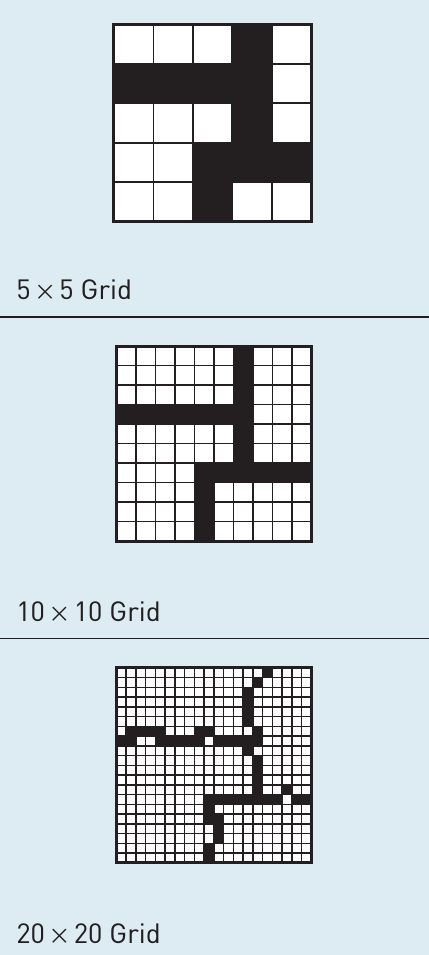
\includegraphics[width=6cm]{RasterResolution.png}
    \caption{Líneas con diferentes dimensiones de celdas. [Fuente: \citet{Heywood2006AnSystems}]}
    \label{fig:rasterResolution}
\end{figure}

% Hay varias variantes de la estructura de datos ráster de la cuadrícula regular, que incluyen: teselación irregular (por ejemplo, red irregular triangulada (TIN)), teselación jerárquica (por ejemplo, árbol cuádruple) y línea de escaneo \citep{Peuquet1991MethodsEnvironment}.

\section{Operaciones geométricas con datos vectoriales}

En esta sección veremos una serie de operaciones que transforman los datos vectoriales. Los resultados de algunas de estas operaciones son nuevas capas cuyas geometrías aportan información adicional a las geometrías originales, o bien las transforman para que su uso sea más adecuado en otros análisis u operaciones.

Existe una amplia gama de funciones para el análisis de datos disponibles en la mayoría de los paquetes SIG, que incluyen técnicas de medición, consultas de atributos, análisis de proximidad, operaciones de superposición y el análisis de modelos de superficies y redes \citep{Heywood2006AnSystems}. A continuación, se explican en qué consisten algunas de las técnicas sin profundizar en la complejidad de los algoritmos que son utilizados detrás de ellas.

\subsection{Medición}

El uso de las operaciones de medición es muy común en los SIG. En un vector, las distancias se miden utilizando el teorema de Pitágoras para obtener la distancia euclidiana. La geometría también se utiliza para calcular perímetros y áreas. Los perímetros se forman a partir de la suma de las longitudes de líneas rectas, y las áreas se calculan sumando las áreas de formas geométricas simples formadas por la subdivisión de la característica de interés \citep{Heywood2006AnSystems}.

Estas medidas, por lo general, son almacenadas como atributos de las entidades espaciales evitando así realizar el cálculo constantemente en cada consulta. Un detalle a tener en cuenta es que al almacenar estos atributos, cualquier modificación de geometría en la entidad debe ir seguida de la actualización de sus medidas de forma manual, de tal forma a mantener la consistencia en los datos.

\subsection{Zona de influencia}

La zona de influencia, conocida como \textit{buffering}, consiste básicamente en una región o polígono alrededor de una entidad. El término es relativamente simple, pero computacionalmente hablando resulta complejo. 

Para una entidad del tipo \textit{Point} su \textit{buffer} consiste en un círculo cuyo radio es la medida máxima de influencia definida. La creación de \textit{buffer} sobre los tipos \textit{Line} y \textit{Polygon} resultan conceptualmente similares, aunque los algoritmos subyacentes son notablemente más complejos (Ver Figuras \ref{fig:pointBuffer}, \ref{fig:lineBuffer} y \ref{fig:polygonBuffer}).

La distancia de \textit{buffer} puede ser variable conforme a valores numéricos incluidos en la tabla de atributos de la capa vectorial para cada entidad. Por ejemplo, con una capa de puntos que representen antenas de distintas potencias y alcances, pueden generarse zonas de influencia con radio distinto. En la Figura \ref{fig:lineBuffer}, se puede observar otro ejemplo donde la línea representa un río con el tamaño de \textit{buffer} definido en base a su caudal.

Los \textit{buffer} en torno a entidades poligonales se extienden normalmente hacia el exterior del borde del polígono aunque también es posible crear zonas de \textit{buffer} hacia el interior del borde del polígono.

\begin{figure}[H]
    \centering
    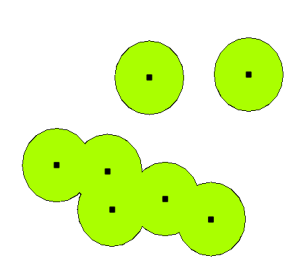
\includegraphics[width=5.5cm]{point_buffer.png}
    \caption{Representación de \textit{buffer} en puntos en el sistema vectorial. [Fuente: Documentación de QGis]}
    \label{fig:pointBuffer}
\end{figure}
% https://docs.qgis.org/2.14/es/docs/gentle_gis_introduction/vector_spatial_analysis_buffers.html

\begin{figure}[H]
    \centering
    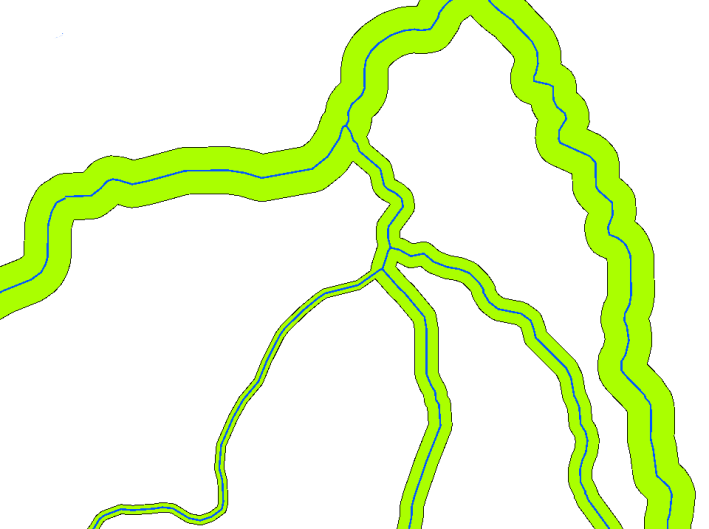
\includegraphics[width=5.5cm]{variable_line_buffer.png}
    \caption{Representación de \textit{buffer} variable en líneas en el sistema vectorial. [Fuente: Documentación de QGis]}
    \label{fig:lineBuffer}
\end{figure}

\begin{figure}[H]
    \centering
    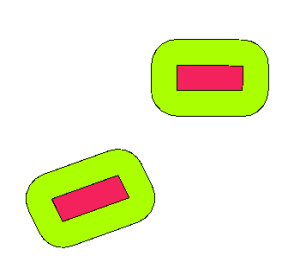
\includegraphics[width=5.5cm]{polygon_buffer.png}
    \caption{Representación de \textit{buffer} en áreas en el sistema vectorial. [Fuente: Documentación de QGis]}
    \label{fig:polygonBuffer}
\end{figure}

\subsection{Superposición}

Estas operaciones permiten generar nuevas capas vectoriales a partir de la fusión de datos de dos o más capas de datos de entrada, pudiendo dichas capas de origen contener distintos tipos de entidades. En los sistemas basados en vectores, la superposición de mapas requiere mucho tiempo, es compleja y computacionalmente costosa. En los sistemas basados en ráster, es justo lo contrario: rápido, directo y eficiente \citep{Heywood2006AnSystems}.

Ejemplos típicos de superposición espacial son:

\begin{itemize}
    \item Intersección: La capa de salida contiene todas las áreas donde ambas capas se solapan (intersectan).
    \item Unión: La capa de salida contiene todas las áreas de las dos capas de entrada combinadas.
    \item Diferencia simétrica: La capa de salida contiene todas las áreas de las capas de entrada excepto aquellas áreas en que ambas capas se solapan (intersección).
    \item Diferencia: La capa de salida contiene todas las áreas de la primera capa de entrada que no se solapan (intersectan) con la segunda capa de entrada.
\end{itemize} 
% \ref pagina de QGIS

\begin{figure}[H]
    \centering
    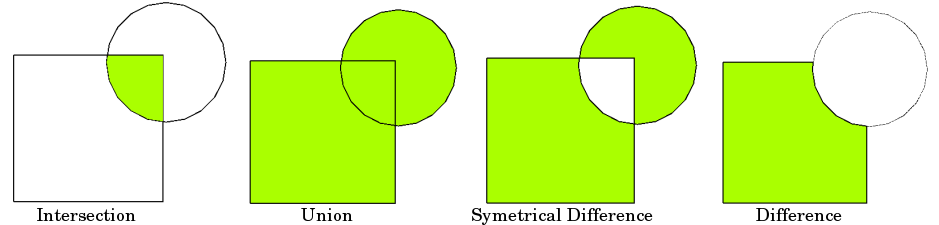
\includegraphics[width=10.5cm]{overlay_operations.png}
    \caption{La superposición espacial con dos capas de entrada vectoriales. La capa vectorial resultante se muestra en verde. [Fuente: Documentación de QGis]}
    \label{fig:overlay}
\end{figure}

% \subsection{Disolución}

% Esta operación recibe este nombre debido a que une polígonos con atributos comunes y disuelve las fronteras existentes entre ellos en una única entidad. No es necesario que exista una frontera entre los polígonos (es decir, que sean contiguos) ya que pueden almacenarse en una capa vectorial entidades compuestas por varios polígonos disjuntos. Esto se puede hacer con cualquier tipo de geometría: puntos, líneas o polígonos.
% % \ref Víctor Olaya

% \begin{figure}[H]
%     \centering
%     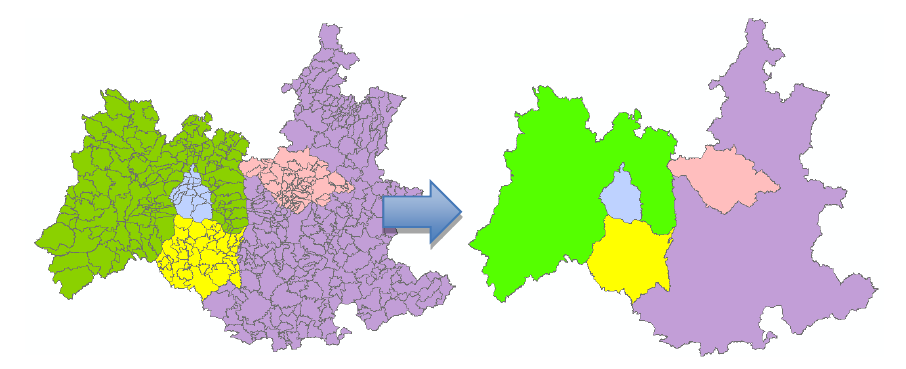
\includegraphics[width=10.5cm]{disolucion_vectorial.png}
%     \caption{Operación de disolución o generalización. [Fuente: Algebra de Mapa. Diplomado]}
%     \label{fig:disolution}
% \end{figure}

\section{Almacenamiento espacial}

Una capa SIG puede ser almacenada con distintos formatos. Tanto para modelos del tipo vectorial como ráster existe un listado extenso de formatos que almacenan datos espaciales. Tal es así, que los software SIG han ido incorporando compatibilidad con los distintos formatos que iban surgiendo para no quedar relegados con otros de la competencia.

Los formatos de archivos SIG ráster mas tradicionales son: 
\begin{itemize}
    \item Esri Grid
    \item GeoTIFF
    \item JPEG 2000
    \item PNG
    \item MrSID
    \item ERDAS IMAGINE (IMG)
    \item ECW
    \item ASCII
    \item GeoPackage
    \item MBTiles
\end{itemize}

Por otro lado, entre los formatos SIG vectoriales más populares están: 
\begin{itemize}
    \item Esri shapefile
    \item CSV/GeoCSV
    \item DWG/DXF/DGN
    \item GML/XML
    \item GPX
    \item GeoPackage
    \item GeoJSON/TopoJSON
    \item GeoRSS
    \item KML/KMZ
    \item MapBox Vector Tiles (MVT)
\end{itemize}

Las capas también pueden ser almacenadas en base de datos relacionales y no relacionales, introduciendo el concepto de base de datos espacial.

% Fuente:https://mappinggis.com/2015/12/los-formatos-gis-raster-mas-populares/

\subsection{Bases de datos espaciales}

Las bases de datos espaciales se utilizan para almacenar datos espaciales. Por lo general, los Sistemas de Gestión de Base de Datos (SGBD) agregan capacidades extras para manejar dicha información. Estas capacidades incluyen, por lo general, estructuración de datos espaciales, índices y funciones para la manipulación y análisis de la información.

El incremento del volumen de los datos ha derivado en la búsqueda de soluciones con alta escalabilidad en algunos \textit{software}. Se requiere que los \textit{software} tengan la capacidad de adaptarse y crecer en capacidad de trabajo o tamaño sin comprometer el rendimiento, funcionamiento y la calidad del mismo. Las bases de datos no han sido la excepción en esta búsqueda, y es así como el uso de las bases de datos conocidas como No-SQL se incrementó debido a las buenas prestaciones para el manejo de grandes volúmenes de datos (\textit{big data}) sobre las tradicionales conocidas como relacionales. 
% Existen diferentes bases de datos No-SQL según su orientación: orientadas a documentos, a grafos, a columnas, entre otros.

Las bases de datos (conocidas con el acrónimo BD y también utilizadas como sinónimo de SGBD) espaciales relacionales siguen y seguirán siendo muy utilizadas por las ventajas que ofrecen sobre las demás en ciertos aspectos. A continuación, se mencionan características que difieren en ambas, pero que pueden variar con el paso del tiempo:

\begin{itemize}
    \item Las BD relacionales mantienen un formato único estructurado interno para almacenar la información geográfica, mientras que las No-SQL no lo tienen.
    \item Las BD No-SQL en ocasiones soportan algunas funcionalidades geométricas para gestionar datos geográficos sencillos. Las BD relacionales tienen una capacidad de análisis espacial mucho más sofisticada, funcionando como un auténtico SIG.
    \item Los SIG más utilizados para análisis espaciales complejos soportan conexiones con bases de datos relacionales, mientras que con No-SQL aún no son muy comunes dichos servicios.
\end{itemize}

Las bases de datos relacionales PostgreSQL y Oracle agregan extensiones para soporte SIG que son PostGIS y Oracle Spatial and Graph, respectivamente. En el caso de PostGIS, al agregarse como extensión a una base de datos en PostgreSQL, agrega un conjunto de funciones espaciales, tablas (donde almacenan las referencias espaciales SRID) y vistas (tablas lógicas que identifican las columnas geométricas de las diferentes tablas de la instancia de base de datos).

Actualmente existen estándares que definen este conjunto de tipos de datos y funciones espaciales mínimas para una base de datos SIG. El Open Geospatial Consortium (OGC) es un consorcio internacional de la industria cuyo objetivo es tratar de estandarizar la forma en que los datos geométricos y espaciales son accedidos y distribuidos. OGC cuenta con numerosas especificaciones que definen el acceso a los datos geoespaciales, servicios web para consulta y manipulación de datos, formatos de datos geoespaciales y consulta de datos geoespaciales.

\section{Mapas y Servidores de mapas}

Miles de páginas Web en internet incorporan mapas en sus sitios con diferentes fines. Estos sitios utilizan simplemente mapas del mundo preexistentes, es decir, no son mapas creados por el sitio, sino que en su mayoría utilizan servicios de mapas que están disponibles para incorporarlos en los diferentes \textit{software}.

Un mapa muy conocido es OpenStreetMap (también conocido como OSM), consiste en un proyecto colaborativo para crear mapas editables y libres. En lugar del mapa en sí, los datos generados por el proyecto se consideran su salida principal. Tanto las imágenes creadas como los datos vectoriales almacenados en su base de datos se distribuye bajo Licencia Abierta de Bases de Datos (ODbL; \textit{Open Database License}).

Otro proyecto de mapa del mundo con una larga trayectoria es Google Maps. Google Maps consiste en un servidor de aplicaciones de mapas en la web que pertenece a Alphabet Inc. Ofrece imágenes de mapas desplazables, así como fotografías por satélite del mundo e incluso la ruta entre diferentes ubicaciones, condiciones de tráfico en tiempo real y un calculador de rutas a pie, en coche, bicicleta y transporte público y un navegador GPS.

Proyectos como éstos ofrecen un listado de funcionalidades gratuitas y pagas. Algunas funcionalidades de ejemplo suelen ser obtener información del tráfico, camino más corto entre un punto de inicio y otro de llegada, ubicación de lugares por nombre, ubicación de calles, entre otros.

Del mismo modo, existen herramientas que permiten alojar nuestros propios mapas en un servidor y brindar servicios de mapa. Uno de ellos es GeoServer, el cual consiste en un servidor de código abierto escrito en Java que permite a los usuarios compartir y editar datos geoespaciales. Está diseñado para la interoperabilidad, publica datos de cualquier fuente de datos espaciales usando estándares abiertos. GeoServer es una implementación compatible con OGC de una serie de estándares abiertos, como el \textit{Web Feature Service} (WFS), el \textit{Web Map Service} (WMS), el \textit{Web Map Tile Service} (WMTS) y el \textit{Web Coverage Service} (WCS). % Optimización PSO

\clearpage
\lhead{\emph{Problemas de rutas}} 
\renewcommand\chaptername{Capítulo}%título "Capítulo"
\chapter{Problemas de rutas}
\label{chap4}
\ifpdf
  \graphicspath{{Chapter4/Chapter4Figs/PNG/}{Chapter4/Chapter4Figs/PDF/}{Chapter4/Chapter4Figs/}}
\else
  \graphicspath{{Chapter4/Chapter4Figs/EPS/}{Chapter4/Chapter4Figs/}}
\fi

\markboth{\hfill \thechapter. Problemas de rutas}{\hfill \thechapter. Problemas de rutas}

Los problemas de rutas son todos aquellos de optimización que se plantean cuando existen unos clientes que demandan un servicio y se debe encontrar la mejor ruta para satisfacerles. Algunos ejemplos típicos son el reparto de correo, la recogida de basura o el transporte escolar, también sirve para modelar otras situaciones como la producción de circuitos electrónicos integrados o la secuenciación de tareas \citep{CalvinoM2011CooperacionPanoramica}. En este capítulo se presentan conceptos básicos de los problemas de rutas y de optimización.

Los problemas de rutas se modelan en un grafo G = (V, A), donde existe un coste no negativo asociado a los arcos y aristas del grafo. Estos problemas se dividen en dos clases: los problemas de rutas por nodos y los problemas de rutas por arcos, que se muestran en el Tabla \ref{table:calsifiacionProblemasRutas}. En el primero de los casos, la ruta óptima a determinar debe visitar todos los nodos, mientras que en el segundo, se deben recorrer todos los arcos del grafo que define el problema. En otras palabras, en los problemas sobre los nodos se entiende que cada cliente está representado por un nodo mientras que en los problemas sobre los arcos se entiende que los arcos son calles que deben ser visitadas \citep{CalvinoM2011CooperacionPanoramica}.

\begin{table}[H]
\caption{Clasificación de problemas de ruta. [Fuente: \cite{CalvinoM2011CooperacionPanoramica}] }
\centering 
\begin{tabular}{cccc}
\hline
Demanda                & \begin{tabular}[c]{@{}c@{}}Restricciones\\ de capacidad\end{tabular} & Nombre habitual del problema                                                                          & Otras restricciones   \\ \hline
\multirow{2}{*}{Nodos} & NO                                                                   & \begin{tabular}[c]{@{}c@{}}Problema del Vendedor Viajante\\ TSP\end{tabular}                          &                       \\ \cline{2-3}
                      & SÍ                                                                   & \begin{tabular}[c]{@{}c@{}}Problema de rutas de vehículos\\ VRP\end{tabular}                          & Recogida/distribución \\ \hline
\multirow{3}{*}{Arcos} & \multirow{2}{*}{NO}                                                  & \begin{tabular}[c]{@{}c@{}}Una componente conexa\\ (Problema del Cartero Chino CPP)\end{tabular}      & Ventanas de tiempo    \\ \cline{3-3}
                      &                                                                      & \begin{tabular}[c]{@{}c@{}}Varias componentes conexas\\ (Problema del Cartero Rural RPP)\end{tabular} & Otras                 \\ \cline{2-3}
                      & SÍ                                                                   & \begin{tabular}[c]{@{}c@{}}Problema de rutas con capacidades\\ CARP\end{tabular}                      &                       \\ \hline
\end{tabular}
\label{table:calsifiacionProblemasRutas}
\end{table}

\section{Problemas de ruta por arcos}

Los problemas de ruta sobre arcos tienen su origen en el siglo XVIII, en la ciudad de Königsberg, donde un río atravesaba la ciudad dividiendo la misma en varias partes, para conectar las partes se contaba con siete puentes (ver Figura \ref{fig:puentesKonigsberg}). Los ciudadanos se preguntaban si es que se podía atravesar todos los puentes pasando sólo una vez por cada uno de ellos.

\begin{figure}[H]
\centerline{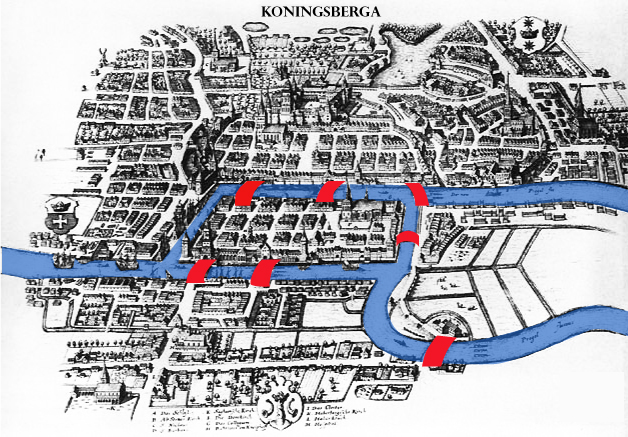
\includegraphics[width=\textwidth]{Konigsberg_bridges.png}}
\caption{Los puentes de Königsberg. [Fuente: \citep{KonigsbergBridges}]}
\label{fig:puentesKonigsberg}
\end{figure}

Leonhard Euler demostró que no era posible, formuló una versión generalizada del problema que establece lo siguiente: si hay dos nodos de grado impar en un grafo, es posible encontrar un camino que atraviese todos los puentes exactamente una vez, empezando en uno de esos nodos y terminando en el otro, esto se conoce como camino euleriano. Si no hay nodos de grado impar, tal camino existe partiendo desde cualquier nodo y terminando en el mismo, esto se conoce como ciclo euleriano. 

En la Figura \ref{fig:grafoPuentesKonigsberg} se observa una representación del grafo de los puentes, en donde cada arco representa a cada uno de ellos. Como los vértices tienen un número de grado impar, es imposible realizar lo que los ciudadanos se planteaban.

\begin{figure}[H]
\centerline{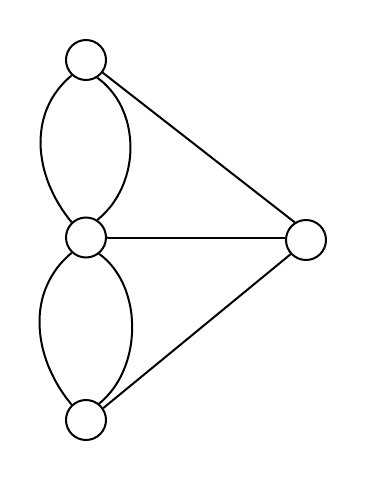
\includegraphics[width=0.6\textwidth]{puentes_grafo.png}}
\caption{Representación del grafo de los puentes de Konigsberg.}
\label{fig:grafoPuentesKonigsberg}
\end{figure}

\subsection{Problema del Cartero Chino (CPP)}

El problema del cartero chino, también conocido como problema del circuito del cartero, el problema de los correos o problema de la inspección y selección de rutas, es el primer problema de rutas por arcos en el que se plantea la posibilidad de construir un ciclo euleriano con coste óptimo \citep{YordaPerez2014ElChino}. 

El problema original dio lugar a multitud de variantes:

\begin{itemize}
    \item CPP en un grafo no dirigido.
    \item CPP en un grafo dirigido.
    \item CPP en un grafo mixto.
\end{itemize}

\subsection{Problema del Cartero Rural (RPP)}

En algunos casos no es necesario atravesar todas las aristas, o arcos, sino solo un subconjunto de ellos (que denominaremos como aristas o arcos requeridos y denotaremos por $A_R$). Sea el grafo G(V, A) un grafo conexo con costes asociados no negativos, en este problema nos interesa definir un ciclo que recorra todos los arcos y/o aristas de $A_R$ al menos una vez. El RPP puede plantearse como un cartero que tiene que repartir el correo en varios pueblos, tiene que recorrer todas las calles de los pueblos, pero no todas las carreteras que los unen.

En general se trata de un problema NP-duro, sin embargo si es un grafo estrictamente dirigido o no dirigido se puede resolver en tiempo polinómico siempre y cuando el subgrafo formado por las aristas o arcos requeridos sea fuertemente conexo. Sus variantes son:

\begin{itemize}
    \item RPP no dirigido.
    \item RPP dirigido (DRPP).
    \item RPP mixto.
\end{itemize}


\subsection{Problema de Rutas por Arcos con Capacidades (CARP)}

En el CARP a cada arco del grafo se le asocia una cantidad no negativa $q_{ij}$, que representa la demanda de cada uno de los clientes. Una flota de vehículos con capacidad Q debe visitar todos los arcos repartiendo (o recogiendo) las cantidades correspondientes sin exceder nunca la cantidad Q \citep{YordaPerez2014ElChino}.
% \section{Modelado de redes}

% Cualquier estructura de red puede describirse utilizando dos tipos de objetos, ver ``Fig.~\ref{fig:arcos_y_nodos}'':

% \begin{itemize}
%     \item Nodos: puntos definidos en la red, por ejemplo las esquinas en donde intersectan calles.
%     \item Arcos: Un arco conecta dos nodos, por ejemplo, una carretera que conecta dos almacenes.
% \end{itemize}

% \begin{figure}[H]
% \centerline{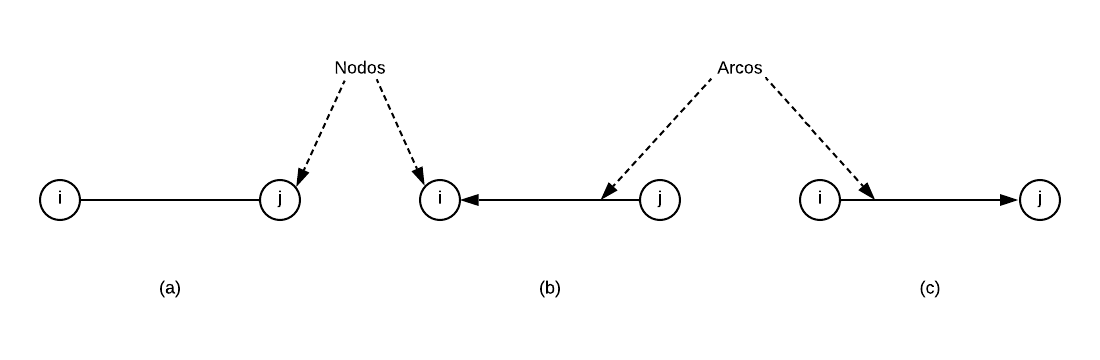
\includegraphics[width=17cm]{arcos_y_nodos.png}}
% \caption{(a) Arco no dirigido. (b) y (c) Arcos dirigidos.}
% \label{fig:arcos_y_nodos}
% \end{figure}

% Una secuencia de arcos que conectan dos nodos se denomina cadena. Cada arco en una cadena comparte exactamente un nodo con el arco anterior.

% Cuando todos los arcos de una cadena se dirigen de tal manera que es posible atravesar la cadena en las direcciones de los arcos desde el nodo de inicio hasta el nodo final, se denomina camino. En la ``Fig.~\ref{fig:caminos}'' se observan dos caminos de A a D:

% \begin{enumerate}
%     \item ABCD
%     \item ABEFD
% \end{enumerate}

% \begin{figure}[H]
% \centerline{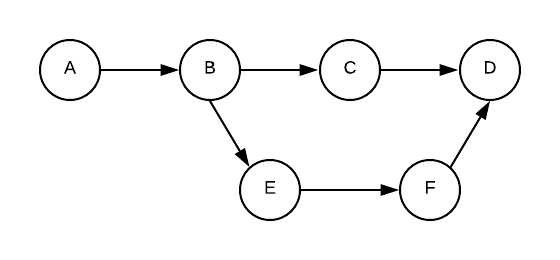
\includegraphics[width=8cm]{Caminos.png}}
% \caption{Caminos}
% \label{fig:caminos}
% \end{figure}

\section{Optimización}

% La optimización es una herramienta importante en la ciencia de la decisión y en el análisis de los sistemas físicos. Para usarlo, se debe identificar algún objetivo, una medida cuantitativa del rendimiento del sistema en estudio. Este objetivo podría ser el beneficio, el tiempo, la energía potencial o cualquier cantidad o combinación de cantidades que se puedan representar con un solo número. El objetivo depende de ciertas características del sistema, llamadas variables o incógnitas. Nuestro objetivo es encontrar valores de las variables que optimicen el objetivo. A menudo las variables están restringidas de alguna manera \citep{Nocedal1999NumericalOptimization}.
La optimización es una herramienta importante en la ciencia de la decisión y en el análisis de los sistemas físicos. Los problemas de optimización se componen generalmente de estos tres componentes \citep{Ramos2010ModelosOptimizacion}:

\begin{itemize}
    \item Función objetivo: Es la medida cuantitativa del funcionamiento del sistema que se desea optimizar (maximizar o minimizar).
    \item Variables: Representan las decisiones que se pueden tomar para afectar el valor de la función objetivo.
    \item Restricciones: Representan el conjunto de relaciones (expresadas mediante ecuaciones e inecuaciones) que ciertas variables están obligadas a satisfacer.
\end{itemize}

El modelado de un problema dado consiste en el proceso de identificar el objetivo, variables y restricciones. La construcción de un modelo es el primer paso para el proceso de optimización, luego se utiliza un algoritmo para encontrar su solución. Existen numerosos algoritmos, cada uno de los cuales se adapta a un tipo particular de problema de optimización \citep{Nocedal1999NumericalOptimization}.

Después de que se haya aplicado un algoritmo de optimización al modelo, debemos ser capaces de reconocer si ha tenido éxito en su tarea de encontrar una solución. En muchos casos, hay expresiones matemáticas que se conocen como condiciones de optimalidad para verificar que el conjunto actual de variables sea la solución del problema. Finalmente, el modelo puede mejorarse aplicando técnicas como el análisis de sensibilidad, que revela la sensibilidad de la solución a los cambios en el modelo y los datos \citep{Nocedal1999NumericalOptimization}.

Un modelo es infactible cuando no existen soluciones que satisfagan todas las restriciones. Esto puede ocurrir debido a que la formulación es incorrecta o los datos no son los correctos.

% \section{Formulación matemática}

% La optimización es la minimización o maximización de una función sujeta a restricciones en sus variables.

La formulación matemática para un problema de optimización puede ser descrito como sigue:

\begin{equation} \label{min}
\min_{x \in \mathbb{R}^n} f(x) 
\end{equation} 

sujeto a 

\begin{equation} \label{sujeto}
\begin{aligned}
    c_{i}(x) = 0, i \in \xi \\
    c_{i}(x) \geq 0, i \in \mathcal{I}
    \end{aligned}
\end{equation}

Aquí $f$ y cada $c_{i}$ son funciones de valores escalares de las variables $x$. $\mathcal{I}$ y $\xi$ son conjuntos de índices.

En (\ref{min}) y (\ref{sujeto}) se utiliza la siguiente notación:

\begin{itemize}
    \item $x$ es el vector de variables, es decir, variables o desconocidos.
    \item$f$ es la función objetivo, una función de $x$ que queremos minimizar o maximizar.
    \item$c$ es el vector de restricciones que las variables deben satisfacer. Esta es una función vectorial de las variables $x$. El número de componentes en $c$ es el número de restricciones individuales que colocamos en las variables.
\end{itemize}

Los métodos de optimización los podemos clasificar en: métodos clásicos y métodos metaheurísticos. Dentro de los primeros se encuentra la optimización lineal, lineal entera mixta, no lineal, estocástica, dinámica. En el segundo grupo se incluyen los algoritmos evolutivos (genéticos, entre otros), el método del recocido simulado (SA), las búsquedas heurísticas (método tabú, búsqueda aleatoria, avariciosa, etc.) o los sistemas multiagente. \citep{Ramos2010ModelosOptimizacion}.

Los problemas de optimización se pueden clasificar según diferentes enfoques. Uno de los enfoques está basado en los valores permitidos para las variables de decisión, donde los problemas de optimización pueden clasificarse como problemas de programación entera o problemas de programación de valores reales \citep{Rao2009EngineeringEdition}.

Si algunas o todas las variables de decisión $x_1$, $x_2$,...$x_n$, solo pueden tomar valores enteros (o discretos), el problema es uno de programación de enteros. Por otro lado, si todas las variables de decisión pueden tomar cualquier valor real, el problema de optimización se denomina problema de programación de valor real.

\subsection{Programación entera (IP)}

Los tipos de programas enteros pueden clasificarse en:
\begin{itemize}
    \item Programas lineal de enteros mixtos (MILP): $x_i \geq 0$ y entero para algunas o todas las $i$. 
    \item Programas enteros puros: $x_i \geq 0$ y entero para cada $i$.
    \item Programas enteros 0-1: $x_i \in \{0,1\}$ para cada $i$.
\end{itemize}

La Figura \ref{fig:milp} muestra el espacio de solución factible en el área $S$ de un MILP, donde la variable de decisión $x$ corresponde a un valor entero mientras que la variable de decisión $y$ representa una variable continua. Por otra parte, en la Figura \ref{fig:pil} se representan mediante puntos a los posibles valores solución en el área $S$, donde ambas variables $x_1$ y $x_2$ corresponden a valores enteros.

\begin{figure}[H]
   \captionsetup[figure]{labelformat=empty}
   \centering
       \subfigure[][]{
            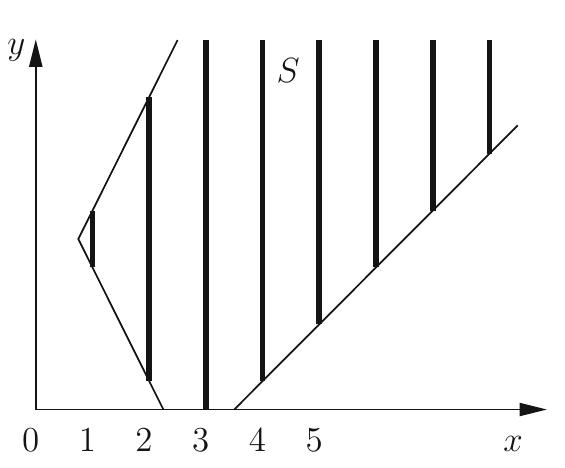
\includegraphics[width=0.45\textwidth]{milp.png}
            \label{fig:milp}
        }
        \subfigure[][]{
            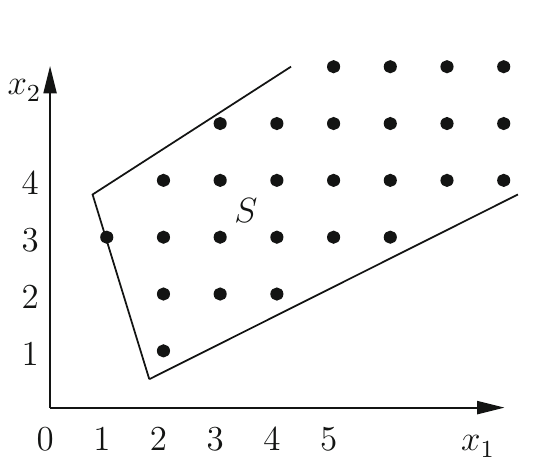
\includegraphics[width=0.45\textwidth]{pil.png}
            \label{fig:pil}
        }
   \caption{Espacion de solución factible. (a) Conjunto lineal de enteros mixto. (b) Conjunto lineal entero puro. [Fuente: \cite{Conforti2014IntegerProgramming}]}
   \label{fig:milp_ip}
\end{figure}

Una programación lineal entera pura es un problema de la forma:

\begin{equation} \label{programacion_entera}
\begin{aligned}
             \max\: & \mu x \\ 
        sujeto\:a\: & Ax \leq b \\
                    &\: x \geq 0\: entero
\end{aligned}
\end{equation}

donde los datos, generalmente racionales, son el vector fila $\mu = (\mu_1,...,\mu_n)$, la matriz $mxn$ $A=(a_{ij})$, y el vector columna $b=(b_1,..., b_m)$. El vector columna $x=(x_1,...,x_n)$ contiene las variables a ser optimizadas. Se dice que un $n$-vector $x$ es entero cuando $x \in \mathbb{Z}^n$. El conjunto de soluciones factibles $S := \{x \in \mathbb{Z}^n_+ : Ax \leq b\}$ a (\ref{programacion_entera}) es llamado el conjunto lineal entero puro \citep{Conforti2014IntegerProgramming}.

\subsection{Métodos para resolver la programación entera}

% 1.4. Métodos de Programación Integral
A pesar de que un IP limitado tiene solo un número finito de solución factible, la naturaleza entera de las variables dificulta la creación de un algoritmo efectivo que busque directamente entre los puntos enteros factibles del espacio de la solución. En vista de esta dificultad, los investigadores han desarrollado un procedimiento de solución que se basa en explotar el tremendo éxito en la resolución de problemas de LP. La estrategia para este procedimiento se puede resumir en tres pasos:

\begin{enumerate}
    \item Relaje las restricciones de enteros del IP para que el IP se convierta en un LP regular.
    \item Resuelva el modelo LP ``relajado'' resultante e identifique su punto óptimo (continuo).
    \item A partir del punto óptimo continuo, agregue restricciones especiales que forzarán iterativamente el punto extremo óptimo del modelo LP resultante hacia las restricciones enteras deseadas.
\end{enumerate}

Existen dos métodos ampliamente utilizados para generar restricciones especiales que forzarán el punto óptimo del problema de LP relajado hacia la solución entera deseada:

\begin{enumerate}
\item Plano de corte (\textit{Cutting plane}).
\item  Ramificación y Acotación (\textit{Branch and bound}).
\end{enumerate}

En ambos métodos, la restricción agregada eliminará partes del espacio de solución relajada, pero nunca ninguno de los puntos enteros factibles. No se puede afirmar que ninguno de los dos métodos sea uniformemente más efectivo para resolver los IP. Sin embargo, los métodos de \textit{branch and bound} son mucho más exitosos computacionalmente que los métodos de plano de corte. Por este motivo, la mayoría de los códigos comerciales se basan en el uso del procedimiento de \textit{branch and bound}.

% \subsubsection{Algoritmos de Ramificación y Acotación (\textit{branch and bound})}

% Este método comienza relajando el requisito de enteros y tratando el problema como uno de programación lineal (LP, \textit{Linear Programming}). Si todas las variables toman valores enteros, la solución está completa. Si no, el algoritmo comienza una búsqueda de árbol.

% \subsubsection{Algoritmos de Planos de Corte}

% \subsubsection{Algoritmos de Ramificación y Corte (\textit{branch and cut})}

% Este método es un algoritmo exacto que consiste en una combinación de un método de plano de corte y un algoritmo de branch and bound.

% \subsubsection{Algoritmos Heurísticos}



\textbf{
    {\huge
        \begin{center}
        \part[Trabajo propuesto]{
            Trabajo propuesto \\ 
            \huge{}}
        \end{center}
    }
}

\clearpage
\lhead{\emph{Modelado del problema}} 
\renewcommand\chaptername{Capítulo}%título "Capítulo"
\chapter{Modelado del problema}
\label{chap5}
\ifpdf
  \graphicspath{{Chapter5/Chapter5Figs/PNG/}{Chapter5/Chapter5Figs/PDF/}{Chapter5/Chapter5Figs/}}
\else
  \graphicspath{{Chapter5/Chapter5Figs/EPS/}{Chapter5/Chapter5Figs/}}
\fi

\markboth{\hfill \thechapter. Modelado del problema}{\hfill \thechapter. Modelado del problema}

\section{Planteamiento del problema}
% \label{cap:planteamiento}

La fase de recolección de residuos sólidos cumple un rol importante en los aspectos socio-económicos y ambientales de una ciudad. Justamente, según la literatura, gran parte del presupuesto de un municipio va destinada a dicha fase. En consecuencia, se genera la necesidad de una búsqueda permanente por disminuir costos en sus procesos sin afectar la calidad del servicio. 

Hoy en día, la selección de la ruta de recolección se basa en la propia intuición y experiencia de los conductores. En algunas ocasiones esto conlleva a dejar sin servicio algunos puntos de la ciudad por desconocimiento de un nuevo conductor asignado a la zona, que a su vez genera que la comuna asuncena realice quejas acerca de la falta de servicio de recolección en tiempo y forma. También es posible el paso en repetidas veces de forma innecesaria por la misma calle dando lugar a mayores gastos de combustible, como se indica en los círculos rojos de la Figura \ref{fig:trayectoRecoleccion}.

\begin{figure}[tb]
    \centering
    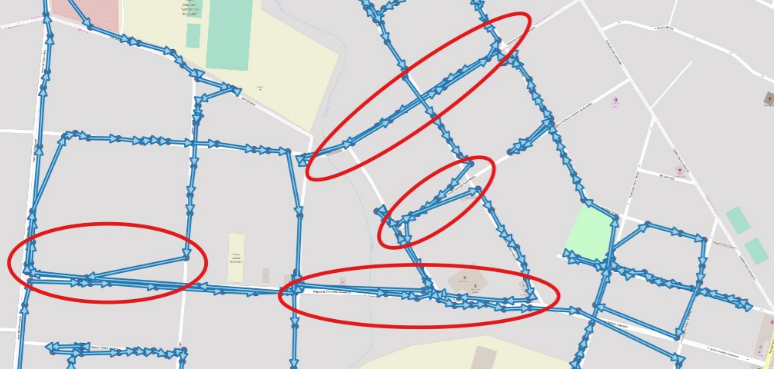
\includegraphics[width=14.5cm]{20170329_recorrido_repetido.png}
    \caption{Trayecto del vehículo 62 en fecha 11 de Julio del 2016 en el turno mañana. [Fuente: Datos de rastreo vía GPS desplegados en la aplicación QGis]}
    \label{fig:trayectoRecoleccion}
\end{figure}

Otra situación muy común es el continuo cambio de circulación en las calles buscando disminuir la congestión del tráfico actual, por ejemplo: cambio de sentido, prohibición de giro a la izquierda, prohibición de giro en U, contramano. También se presentan situaciones donde las calles quedan clausuradas para su uso por motivo de reparación de la capa asfáltica, trabajos de instalación o reparación de cañería.

Por ello se evidencia la necesidad de una herramienta de soporte de decisión que aborde el problema del enrutamiento de los vehículos recolectores teniendo en cuenta el procedimiento actual llevado a cabo para la recolección de residuos domiciliarios de la DSU.

% Para  ello  se  implementa  una  solución  GIS  que  optimice  el  camino  del  vehículo recolector teniendo en cuenta el procedimiento actual llevado a cabo para la recolección de residuos domiciliarios, gestionando de forma sencilla y rápida el estado actual de las calles y sus reglas de circulación.

% En la Figura \ref{fig:trayectoRecoleccion}, se muestra una pequeña parte del rastreo de una zona, en los círculos de color rojo se pueden observar como el mismo vehículo recorre la misma calle más de una vez. Esta situación se pudo contemplar en los recorridos de varias zonas. Para la recolección de datos se solicitó a la DSU el permiso de instalar un dispositivo GPS a un vehículo recolector de basura, como parte de este proyecto, a través del cual obtuvimos por un periodo de 3 meses los datos de posicionamiento relacionados al vehículo 62 de propiedad de la Municipalidad de Asunción. Esta idea ya generó el interés de la Municipalidad de Asunción, que posteriormente ha realizado una licitación para dotar a todos los vehículos recolectores de residuos un dispositivo similar GPS, brindándonos acceso a los datos del rastreo de todos vehículos recolectores.

\section{Metodología de trabajo}

En la Figura \ref{fig:metodologia} se muestra la metodología seguida en este trabajo: la recolección de datos, selección de un modelo matemático adecuado para resolver el problema de ruteo, la implementación de la herramienta \textit{TapeYty}, el despliegue de la ruta óptima y por último el análisis de los resultados.

\begin{figure}[htbp]
\centerline{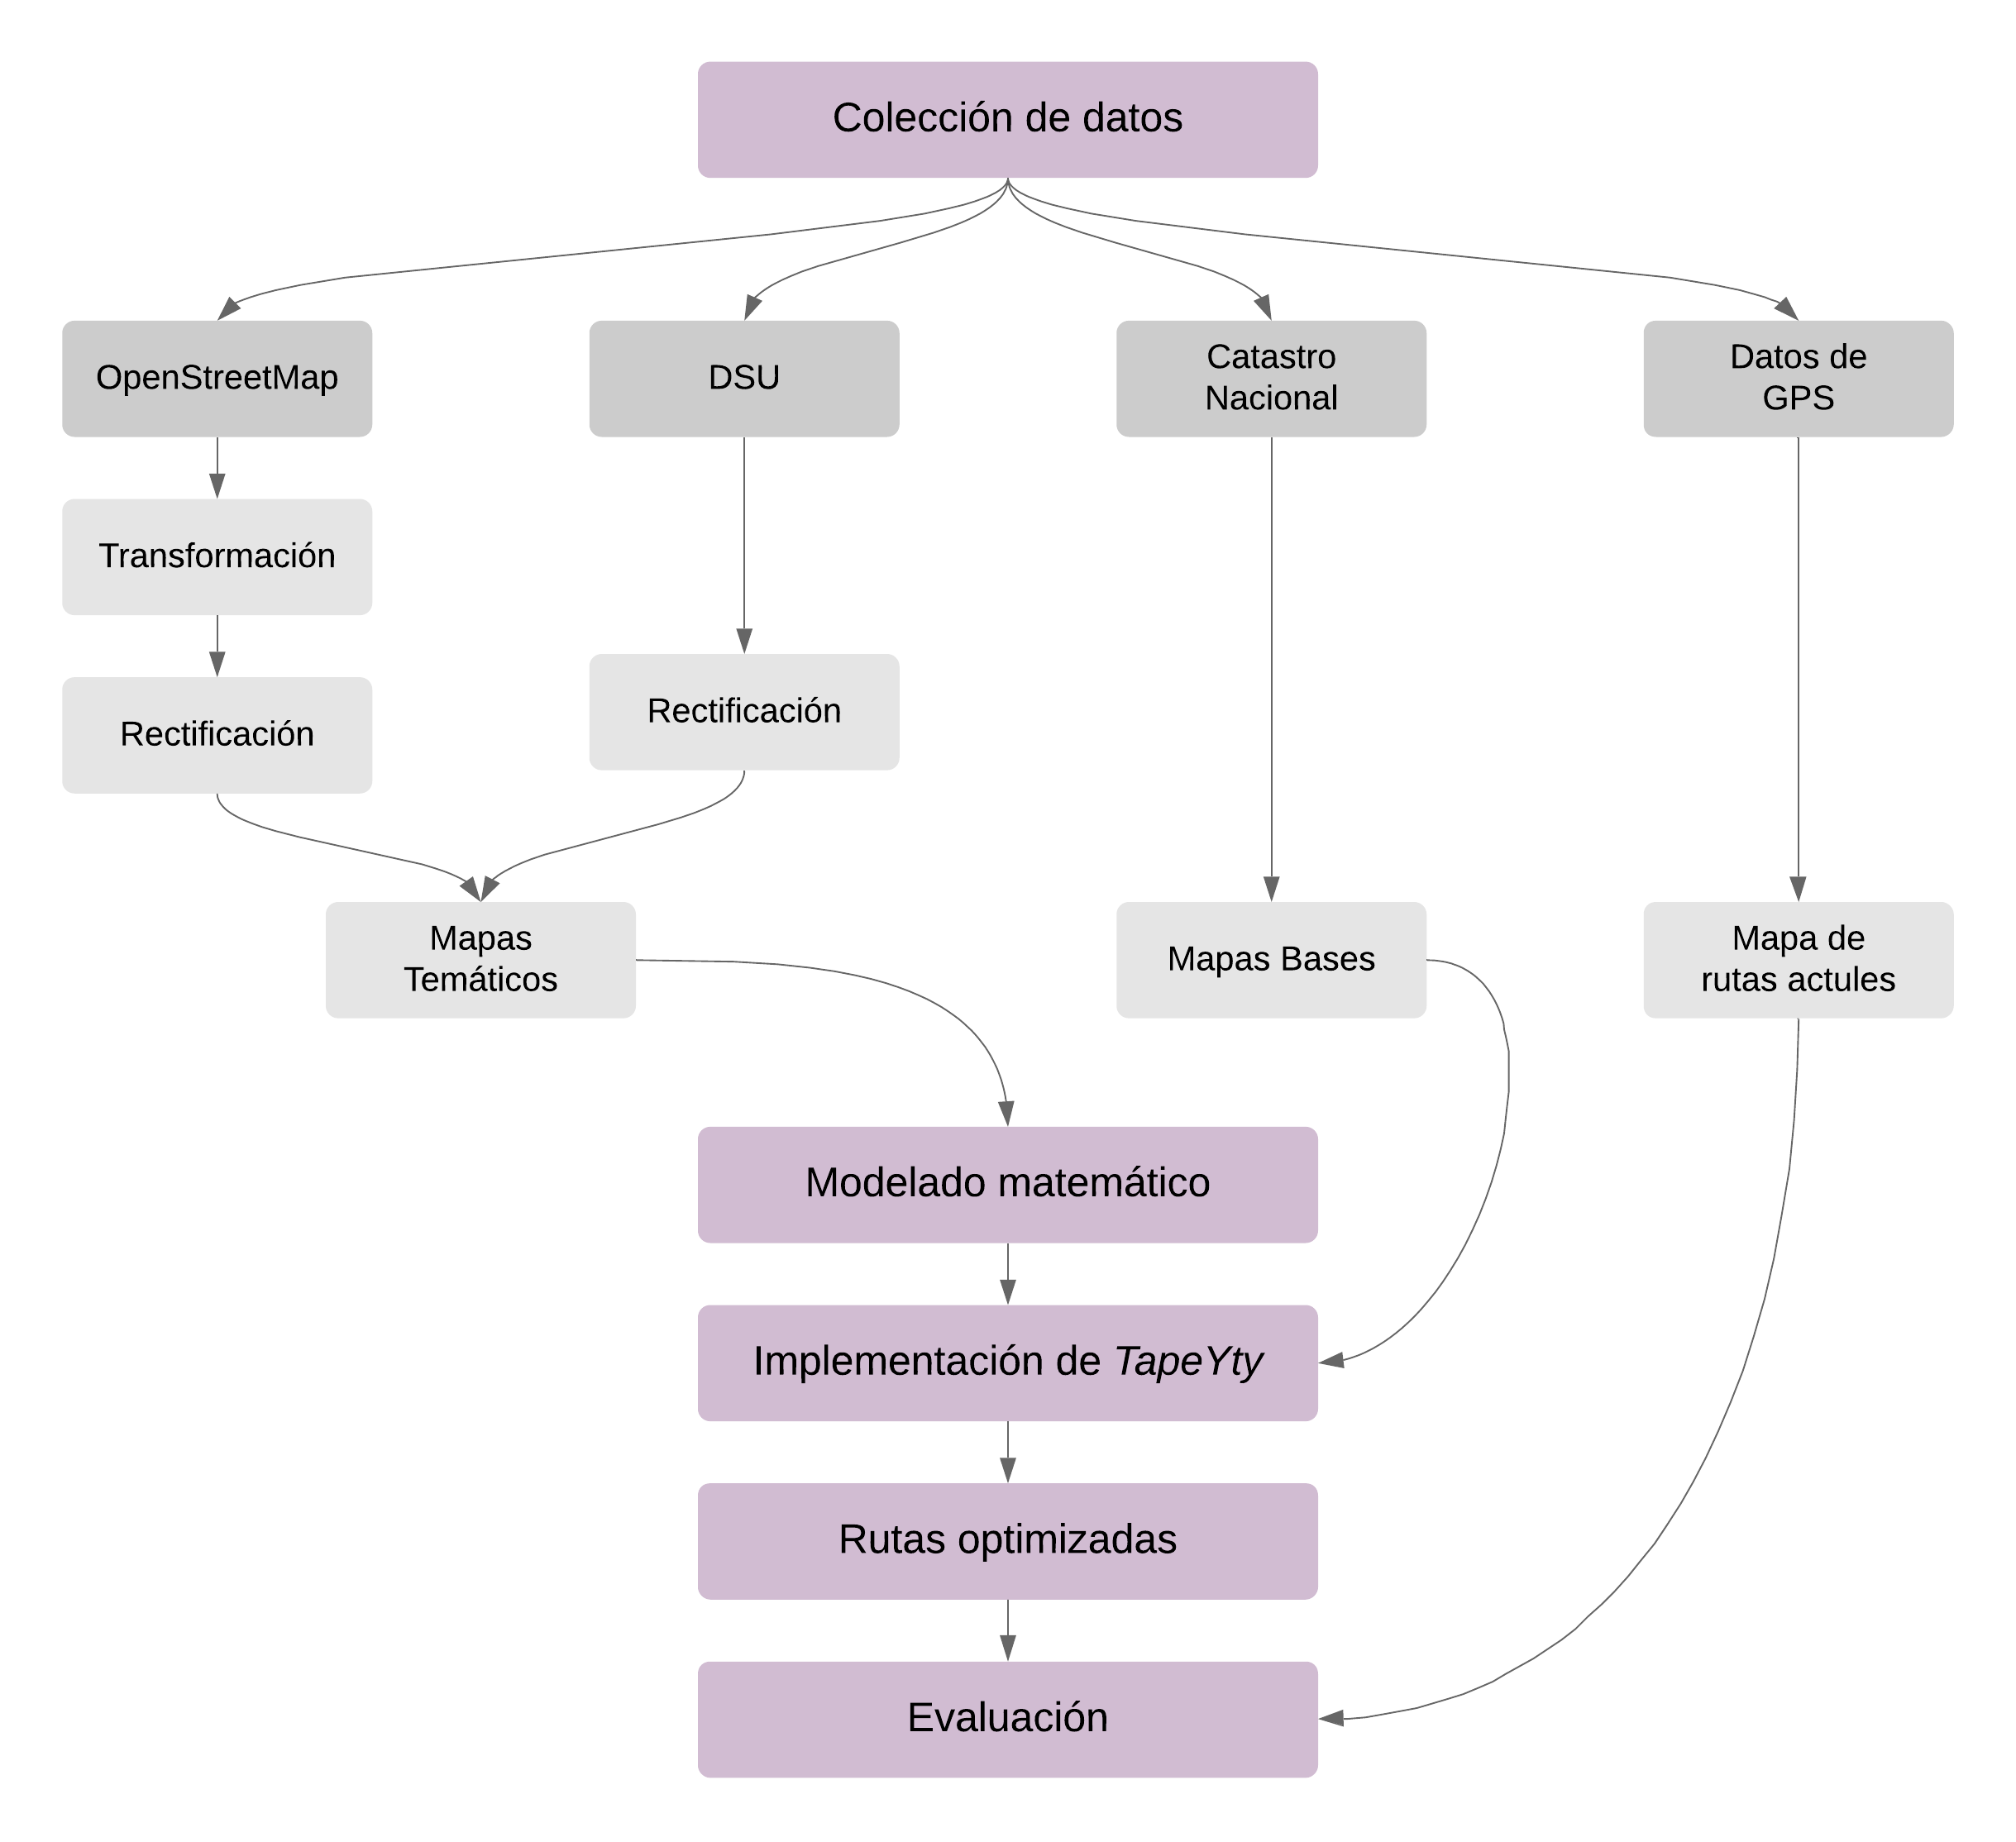
\includegraphics[width=\textwidth]{DiagramaDeMetodologia.png}}
\caption{Vista general de los procesos de la metodología aplicada.}
\label{fig:metodologia}
\end{figure}

% La solución del trabajo de investigación es lo que se buscará encontrar en el transcurso del desarrollo del TFG. La solución encontrada debe permitir obtener mejores resultados en cuanto a costo de recolección, en comparación a la situación actual en la DSU del municipio de Asunción, así como también, generar resultados óptimos que contribuyan con el estado del arte actual

\section{Colección de Datos}

A modo de desplegar las rutas de recolección en el mapa de la aplicación se debe contar necesariamente con un mapa de calles y otro de zonas definidas por la DSU de recolección. Tanto el mapa de zonas como el de calles deben estar almacenados en la base de datos GIS para ser posteriormente utilizados durante el procesamiento de \textit{TapeYty}. Se crea una base de datos espacial utilizando el gestor de base de datos de código abierto PostgreSQL en su versión 10.8 \citep{PostgreSQL}, junto con su extensión PostGIS en su versión 2.4 \citep{PostGIS}, la cual brinda soporte para objetos geográficos.

Primeramente, se necesitó exportar los datos de Asunción desde OSM, debido a que no se tuvo conocimiento de alguna institución que proveyera de mapas de calles de la ciudad con sus sentidos. A continuación se detallan los pasos seguidos para obtener la red de rutas utilizada: 
\begin{enumerate}
    \item Se utiliza la herramienta \textit{osm2pgsql} para importar los datos de OSM a la base de datos, en el sistema de referencia geográfico WGS84 (SRID 4326). 
    \item Se utilizan las funciones de PostGIS para convertir los valores de latitud y longitud al tipo de dato geométrico \textit{Point}. 
    \item Las calles de OSM están representadas por líneas, que a su vez contienen una serie de nodos (puntos). Se excluyen los puntos que no pertenecen a calles de la ciudad, además de puntos superpuestos.
    \item Para un mejor manejo de la red de rutas se crea un proceso de segmentación de las calles, donde cada segmento de calle está formado por pares de nodos consecutivos, se define el sentido del segmento, longitud y si corresponde a un callejón sin salida.
    \item Por último, se realizan las transformaciones correspondientes para almacenar las restricciones de giro y contramano, desde los datos registrados en OSM.
\end{enumerate}

Para almacenar la información de red de calles se definen las siguientes tablas en la base de datos GIS:

\begin{itemize}
    \item Nodo: En esta tabla se almacenan los puntos que se utilizan como extremos de los segmentos de calle. Se almacena la latitud y la longitud.
    \item Segmento: Contiene líneas de calle formada a partir de dos nodos consecutivos. Se almacena el nombre, el nodo origen, el nodo destino, si es de único de sentido y si es sin salida. Si el segmento es de único sentido, entonces el nodo origen y destino definen el sentido del mismo.
\end{itemize}

Al importar los datos desde OSM se detectaron algunos datos incorrectos que generarían inconvenientes para la obtención del recorrido para la recolección de residuos. OSM identifica las calles sin salida por medio del atributo \textit{no\_exit}. Si su valor es \textit{true} representa una calle sin salida, sin embargo muchas calles sin salida lo tienen como \textit{false}. Otra inconsistencia encontrada es con el valor del atributo \textit{one\_way}, donde muchas calles sin salida tienen su valor en \textit{true} indicando que es de único sentido cuando realmente deben ser doble sentido.

Los problemas de datos mencionados se solucionan con sentencias SQL. Para identificar las calles sin salida se realiza una consulta donde se obtengan la unión de: ``todos los segmentos que tengan un nodo inicial que no sea nodo final ni inicial de algún otro segmento'' y ``todos los segmentos que tengan un nodo final que no sea inicial o final de otro segmento''. Se obtiene como resultado la lista de todos los ID (identificadores) de los segmentos sin salida y se almacena en una tabla temporal. Se actualizan los campos de sin salida y sentido de todos aquellos segmentos cuyos ID se encuentran en la tabla temporal.

La delimitación de las zonas de recolección fue proveída por la DSU a través de un archivo \textit{shape} del tipo de dato geométrico \textit{Polygon}. Se realizan los siguientes procedimientos para la limpieza y corrección de los datos geográficos sobre dicha capa:

\begin{enumerate}
\item Se importa el \textit{shape} de Zonas a la base de datos mediante la herramienta \textit{shp2pgsql}, creándose así la tabla de zonas.
\item Se utiliza la opción de autoensamblado de QGIS. Esta opción ayuda a hacer coincidir con precisión los límites de las zonas con las calles de OSM.
% \item Con el programa QGIS, se agregan las capas PostGis de Segmentos, Nodos (de los segmentos) y la nueva de Zonas.
% \item Se configura la opción de autoensamblado de QGIS. Esta opción ayuda para hacer coincidir con precisión la edición de capas con los nodos de los segmentos. Es decir, se utilizan los nodos de los segmentos para hacer coincidir con los nodos de las líneas que formarán el polígono de la zona.
\item En la tabla de zonas se almacenan: nombre, superficie, densidad poblacional, cantidad de lotes y distrito.
\end{enumerate}

Para actualizar la superficie se utiliza la función geométrica de área de polígonos. Para actualizar la cantidad de lotes y distrito se utiliza la función de intersección. No se cuentan con datos de densidad poblacional de todas las zonas de recolección.

Los mapas bases de Departamentos y Distritos son proveídos a la aplicación por el Sistema Nacional de Catastro a través de su portal de datos abiertos.

La DSU cuenta en algunos vehículos de su flota con un sistema de monitoreo mediante GPS: 

\begin{itemize}
    \item Se accede a los datos a través de archivos en formato de plantilla.
    \item Esta información será utilizada para el análisis y comparación de los resultados.
\end{itemize}

\section{Modelo matemático}

Como resultado de la revisión del estado del arte, se utiliza la solución propuesta por \citet{Braier2017AnArgentina} para optimizar el enrutamiento de vehículos recolectores, ya que este modelo contempla las restricciones de la red de rutas, resolviendo una de las debilidades de los enfoques de la programación matemática mencionado en \cite{Sulemana2018OptimalMethods}. Además, la falta de datos relacionados con la cantidad de toneladas recolectadas por zonas fue otro de los principales motivos por el cual se seleccionó un problema de ruta cuya demanda se encuentra sobre los arcos (calles que deben ser visitadas), y además no posea restricciones de capacidad.

El estudio en \cite{Braier2017AnArgentina} presenta similitudes con el caso de estudio de este trabajo, entre ellas es posible citar:

\begin{itemize}
    \item División de la ciudad en sectores y recolección casa por casa: La situación es muy similar, ya que el procedimiento consiste en recoger los residuos domiciliarios casa por casa, debiendo cubrir todas las calles de un conjunto de cuadras o manzanas, denominadas zonas.
    \item Tamaño de problema: Una zona de recolección abarca en promedio el mismo número (entre 40 y 80 cuadras aproximadamente).
    \item Calles, carreteras, caminos: el trabajo de \citet{Braier2017AnArgentina} tomó como caso de estudio la ciudad de Morón el cuál presenta caminos con particularidades muy comunes a otras sudamericanas como la de Asunción: calles sin salida, calles estrechas, peatonales, giros prohibidos, entre otros.
\end{itemize}

Los siguientes supuestos son establecidos:

\begin{itemize}
    \item El vehículo recolector cuenta con capacidad suficiente para recoger los residuos de una zona determinada.
    \item El tráfico es constante en una zona de trabajo en el turno en que se recogen sus residuos.
    \item Las modificaciones geográficas de los datos espaciales estarán a cargo de una persona capacitada en el área GIS.
    % La persona encargada de la administración del sistema posee conocimientos básicos en GIS y podrá actualizar, crear y eliminar una zona de trabajo mediante el sistema \textit{QGis}
\end{itemize}

Cada zona de recolección de la ciudad de Asunción es representada por un grafo mixto $H$ \citep{Braier2017AnArgentina}, cuyos nodos representan las esquinas de las calles en la zona, y los arcos son los segmentos de calles que corren entre dos intersecciones consecutivas. Las calles de un único sentido están representadas por arcos dirigidos y las calles finas de doble sentido por arcos no dirigidos, ya que ambos lados de la calle pueden ser servidos en un solo viaje. En el caso de calles anchas de doble sentido, como las avenidas, cada lado debe ser servido de forma separada, por lo que estas calles se representan con dos arcos dirigidos, una en cada sentido.

Para incorporar las restricciones de regulación de tráfico se construye un grafo dirigido $G$ desde el grafo $H$. El grafo $H$ es expandido dividiendo cada nodo en varios nuevos nodos representando todas las formas en las que se puede llegar y salir de la esquina en cuestión. En la Figura \ref{fig:grafo_expandido}(a) se puede observar un nodo en el grafo original $H$ antes de su expansión y en la Figura \ref{fig:grafo_expandido}(b) el nodo que ha sido expandido en seis nuevos nodos, representando cada posible entrada y salida del nodo. Los arcos auxiliares dirigidos son agregados y conectan los nuevos nodos, representando así las transiciones permitidas de una esquina a otra.

El modelo de programación entera propuesto por \citet{Braier2017AnArgentina} está definido de la siguiente manera:

\subsection{Conjuntos y Parámetros}
\label{sec:conjunto-parametros}

\begin{itemize}
\item $G(V, A)$: Grafo dirigido en el que los nodos V corresponden a todas las alternativas posibles para llegar a las esquinas de las intersecciones y A está compuesto por arcos que se pueden atravesar en una sola dirección específica.

\item $E \subseteq \{ \{i, j\}: i \in V, j \in V, i \neq j\}$: Representan segmentos de calles de dos vías que pueden ser recorridos en cualquier sentido.

\item $AM \subseteq A $: Arcos obligatorios que representan segmentos que deben recorrerse únicamente en el sentido especificado.

\item $w : A \rightarrow \mathbb{R} $: Función de peso que asocia un peso a cada arco, en este caso la distancia del segmento de calle. Los arcos auxiliares entre nodos que representan esquinas tienen un mismo valor ínfimo.

\item $I \subseteq V $: Nodos que especifican los puntos de inicio permitidos para la ruta.

\item $S \subseteq V$: Se define $\delta^+ (S) = \{i j \in A: i \in S , j \notin S \}$ , que representa un conjunto de arcos que van desde nodos en $S$ a nodos en $V \backslash S$.
\end{itemize}

El problema de ruteo es una versión particular del problema del cartero rural abierto dirigido generalizado, ya que el arco $i j \in E $ determina el grupo de arcos $L_{i j} = \{i j, j i\}$, en el que al menos uno de ellos debe ser atravesado en la solución final y además se busca un camino cuyo nodo inicial y final no se especifican.

\begin{figure}[tbp]
\centerline{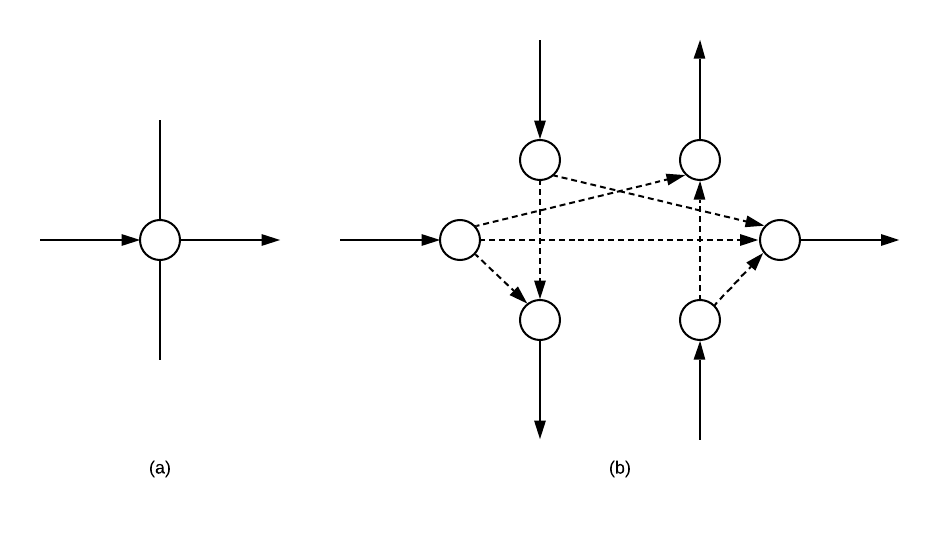
\includegraphics[width=9.5cm]{expanded_graph.png}}
\caption{Expansión de un cruce entre una calle de sentido único y una calle de doble sentido. (a) Grafo mixto original $H$. (b) Grafo dirigido $G$ luego de la expansión, los arcos auxiliares están representados por líneas discontinuas. [Fuente: \citet{Braier2017AnArgentina}]}
\label{fig:grafo_expandido}
\end{figure}

\subsection{Variables de decisión}
\begin{itemize}
\item $x_{i j}$: Para cada arco $ {i j} \in A$ esta variable representa el número de veces que $i j$ es atravesado.

\item $s_i$: Para cada nodo $i \in I$ esta variable binaria especifica si  $i$ es el primer nodo de la ruta.

\item $t_j$: Para cada nodo $j \in V$ esta variable binaria indica si $j$ es el último nodo de la ruta.
\end{itemize}

\subsection{Definición del programa entero}
\label{sec:programa-entero}
\begin{equation*}
\min \sum_{i j \in A} w_{i j} x_{i j}  \\
\end{equation*} 
\hbox{}

\begin{equation} \tag{1} \label{eq1}
\begin{gathered}
x_{i j} \geq 1 \\
\forall i j \in A M
\end{gathered}
\end{equation} 
\hbox{}

\begin{equation} \tag{2} \label{eq2}
\begin{gathered}
x_{i j} + x_{j i} \geq 1 \\
\forall i j \in E
\end{gathered}
\end{equation}
\hbox{}

%ecuacion 3a
\begin{equation} \tag{3a} \label{eq3a}
\begin{gathered}
s_i + \sum_{j: j i \in A} x_{j i} = \sum_{j: i j \in A} x_{i j} + t_i \\
\forall i \in I
\end{gathered}
\end{equation} 
\hbox{}

%ecuacion 3b
\begin{equation} \tag{3b} \label{eq3b}
\begin{gathered}
\sum_{j: j i \in A} x_{j i} = \sum_{j: i j \in A} x_{i j} + t_i \\
\forall i \in V\backslash I
\end{gathered}
\end{equation}
\hbox{}

\begin{equation} \tag{4} \label{eq4}
\sum_{i \in I} s_i = 1 
\end{equation}
\hbox{}

\begin{equation} \tag{5} \label{eq5}
\sum_{i \in V} t_i = 1 
\end{equation}
\hbox{}

\begin{equation} \tag{6} \label{eq6}
\begin{gathered}
    \sum_{i j \in \delta + (S)} x_{i j} \geq 1 \\
    \forall S \subseteq V
\end{gathered}
\end{equation}
\hbox{}

\begin{equation} \tag{7} \label{eq7}
\begin{gathered}
    x_{i j} \in \mathbb{Z}_+ \\
    \forall i j \in A
\end{gathered}
\end{equation}
\hbox{}

\begin{equation} \tag{8} \label{eq8}
\begin{gathered}
    s_i \in \{0,1\} \\
    \forall i \in I
\end{gathered}
\end{equation}
\hbox{}

\begin{equation} \tag{9} \label{eq9}
\begin{gathered}
    t_i \in \{0,1\} \\
    \forall i \in V
\end{gathered}
\end{equation}

La función objetivo busca minimizar el costo total de la ruta de recolección de residuos. El costo en este trabajo se refiere a la distancia recorrida por el vehículo recolector. La restricción (\ref{eq1}) impone que todos los arcos de único sentido deben ser visitados al menos una vez, la (\ref{eq2}) requiere que los arcos no dirigidos sean atravesados al menos una vez en cualquier sentido. Las restricciones (\ref{eq3a}) y (\ref{eq3b}) aseguran que la solución encontrada es realmente un camino agregando la condición de conservación de flujo estándar a cada nodo. Las restricciones (\ref{eq4}) y (\ref{eq5}) garantizan que el nodo inicial y final sean únicos. Las restricciones (\ref{eq1})-(\ref{eq5}) permiten la formación de subtours, la restricción (\ref{eq6}) es el estándar de eliminación de subtours. Las restricciones (\ref{eq7})-(\ref{eq9}) especifican los valores posibles para las variables del modelo.

\subsection{Algoritmo de solución}
\label{algoritmo-solucion}
% En el modelo dado en la sección \ref{sec:programa-entero} se puede observar la restricción de eliminación de subtours la cual es muy costosa en la generación de las mismas como también en  la complejidad del problema. En este contexto la estrategia propuesta en \cite{Braier2017AnArgentina} se basa en tratar de obtener una solución rápidamente sin considerar el problema de subtour e ir agregando las restricciones sucesivamente, esto se conoce como técnica de agregación dinámica de restricciones a un modelo relajado.

En el modelo dado en la sección \ref{sec:programa-entero} se puede observar la restricción de eliminación de subtours la cual es muy costosa en la generación de las mismas como también en la complejidad del problema. En este contexto la estrategia propuesta en \citet{Braier2017AnArgentina} se basa en tratar de obtener una solución rápidamente sin considerar el problema de subtour, en caso de que existan subtours se eliminan mediante el procedimientos de mezcla de subtours, si no se puede utilizar esta técnica se van agregando las restricciones sucesivamente, esto se conoce como técnica de agregación dinámica de restricciones a un modelo relajado.

Los siguientes pasos detallan la estrategia:

\begin{enumerate}
\item Crear el modelo relajado $M: = (\ref{eq1}) - (\ref{eq5})$ y $(\ref{eq7}) - (\ref{eq9})$.
\item Resolver $M$.
\item Si no se puede encontrar ninguna solución para $M$, retornar ``infactible'' y parar.
\item Si la mejor solución encontrada para $M$ no tiene subtours, retornar esta solución y parar.
\item Si los subtours pueden ser mezclados con el tour que contiene el nodo inicial y final, entonces mezclarlos, retornar la solución obtenida y parar.
\item De lo contrario, agregar a $M$ la restricción de eliminación de subtour estándar (\ref{eq6}) por cada subtour en la solución y regresar al Paso 2.
\end{enumerate}

El procedimiento de mezcla de subtours descrito por \citet{Braier2017AnArgentina}, utilizado en el paso 5, consiste en que dado un subtour \textit{S} y el camino principal \textit{P}, es decir el camino que empieza en el único vértice $i \in I$ con $s_i = 1$, y termina respectivamente en $t_i = 1$, se intenta intercambiar los arcos auxiliares para mezclar \textit{S} y \textit{P}. Se puede presentar una de las siguientes tres configuraciones:

\begin{itemize}
    \item Configuración A: Si el camino principal y el subtour se encuentran en algún nodo intermedio, como en la Figura \ref{fig:procedimiento_mezcla_subtours}(a), entonces son unidos como en la Figura \ref{fig:procedimiento_mezcla_subtours}(b)
    \item Configuración B: Si el subtour se encuentra con el último nodo en la ruta principal, como en la Figura \ref{fig:procedimiento_mezcla_subtours}(c), entonces se unen como en la Figura \ref{fig:procedimiento_mezcla_subtours}(d).
    \item Configuración C: Si el subtour se encuentra con el primer nodo en la ruta principal, como en la Figura \ref{fig:procedimiento_mezcla_subtours}(e), entonces se unen como en la Figura \ref{fig:procedimiento_mezcla_subtours}(f).
\end{itemize}

\begin{figure}[tbp]
\centerline{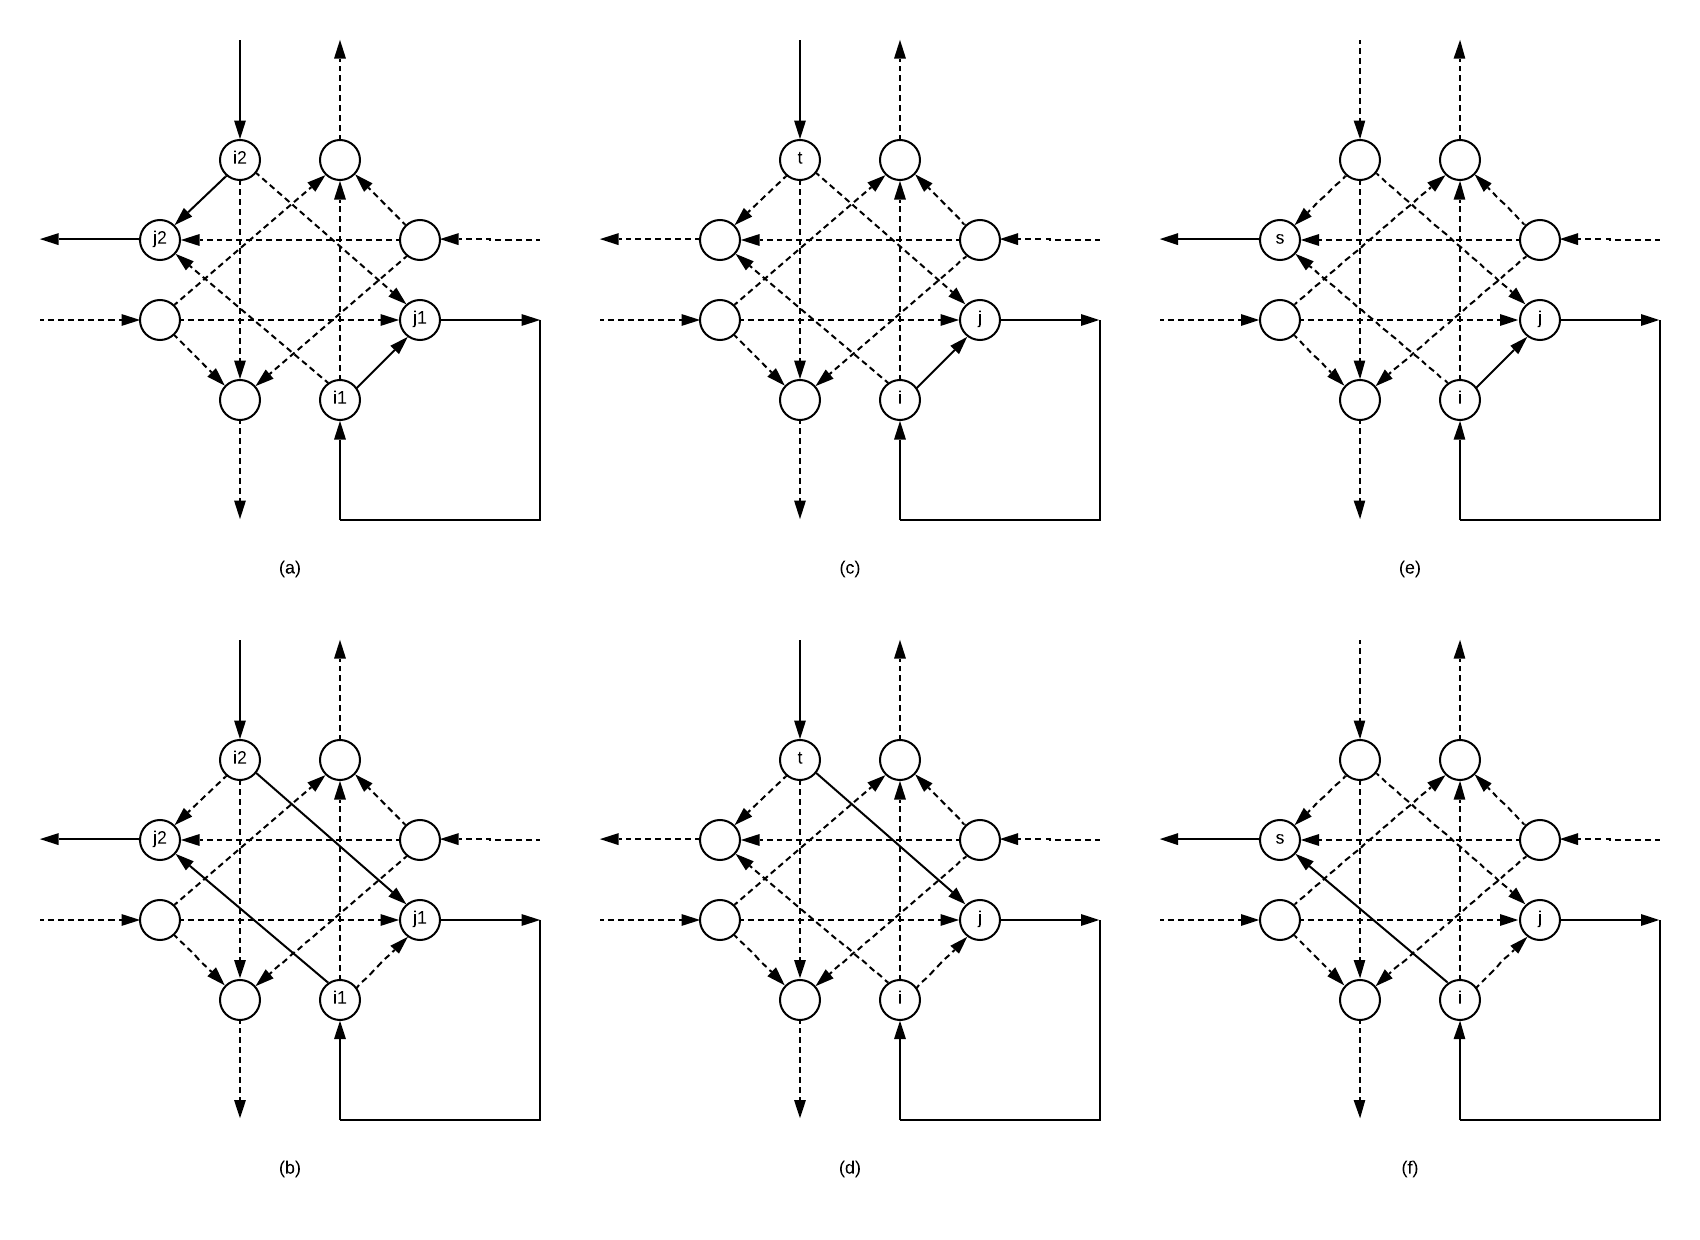
\includegraphics[width=\textwidth]{mezcla_subtours.png}}
\caption{Posibles configuraciones en el procedimiento de la mezcla de subtours. Si \textit{P} y \textit{S} tienen la configuración (a), (b) o (c), entonces la solución es modificada de acuerdo a lo especificado en (b), (d) o (f) respectivamente. [Fuente: \citet{Braier2017AnArgentina}]}
\label{fig:procedimiento_mezcla_subtours}
\end{figure}

Este procedimiento es aplicado para cada subtour en la solución hasta que todos sean mezclados al camino principal, dado que el costo de todos los arcos auxiliares que unen los nodos de las esquinas es el mismo, la ruta modificada permanece óptima, por lo que el algoritmo se detiene y devuelve la solución obtenida en este caso.

Dado que no siempre los subtours pueden ser mezclados con la técnica recién mencionada, el algoritmo principal descrito agrega una restricción estándar de eliminación de subtoures al modelo M, tal y como se especifica en el Paso 6.

Finalmente, en caso que el modelo matemático encuentre una solución factible, el resultado del modelo indica la distancia total, los arcos que son atravesados y el número de veces que estos son atravesados. Sin embargo, para conocer el camino a seguir es necesario encontrar la secuencia del mismo. 

\section{Método de secuenciación}

% En este trabajo se realiza una búsqueda en profundidad para obtener la secuencia a seguir a partir del resultado del problema descrito en la sección anterior. El algoritmo toma como entrada el nodo inicial, nodo final y la cantidad de veces que se atraviesa por cada arco del grafo $G$. Se describe a continuación los pasos del algoritmo:

% En este trabajo se realiza una búsqueda en profundidad para obtener la secuencia a seguir a partir del resultado del problema descrito en la sección anterior. El algoritmo recibe como parámetros de entrada el nodo inicial, nodo final, la cantidad de veces que se atraviesa por cada arco del grafo $G$ y un grafo dirigido $N$ construido teniendo en cuenta solo los arcos atravesados. Se describe a continuación los pasos del algoritmo:

% \begin{enumerate}
% \item Leer el grafo $N$ resultante del GDRPP abierto. 
% \item Inicializar nodo actual al valor del nodo inicial.
% \item Inicializar un vector vacío $seq$, en el que los nodos se almacenarán en el orden en que deben ser visitados.
% \item Agregar a $seq$ el nodo actual.
% \item Si el nodo actual es igual al nodo final y ya se atravesaron todos los arcos, entonces retornar $seq$ y parar.
% \item Sino, tomar uno de los nodos sucesores del nodo actual en $N$, donde el arco formado por el nodo actual y el nodo sucesor aún no haya sido tenido en cuenta, asignar como nodo actual el nodo sucesor y volver al paso 4.
% \end{enumerate}

En este trabajo se utiliza el algoritmo implementado en \cite{RiveraHazim2015APath} que encuentra el camino euleriano de un multigrafo dirigido para obtener la secuencia a seguir. Se genera un multigrafo dirigido $MG$ a partir del resultado del problema descrito en la sección anterior, creando arcos dirigidos según la cantidad de veces que se atraviesa por cada arco del grafo $G$. 

El algoritmo recibe como parámetros de entrada el nodo inicial, nodo final y $MG$. Devuelve como resultado, la secuencia de arcos del recorrido solución. Los siguientes pasos detallan el algoritmo de secuenciación:

\begin{enumerate}
    \item Comience con una pila vacía y un camino (euleriano) vacío. 
    \item Se haya el multigrafo reverso de $MG$ y se trabajo con el mismo. El reverso es un grafo con los mismos nodos y bordes pero con las direcciones de los arcos invertidas.
    \item Se elige el vértice que representa el nodo final.
    \item Si el vértice actual no tiene arcos salientes (es decir, vecinos): agréguelo al camino, elimine el último vértice de la pila y configúrelo como el actual. De lo contrario (en caso de que tenga arcos salientes, es decir, vecinos): agregue el vértice a la pila, tome cualquiera de sus vecinos, elimine el arco entre ese vértice y el vecino seleccionado, y establezca ese vecino como el vértice actual.
    \item Repita el Paso 4 hasta que el vértice actual no tenga más arcos salientes (vecinos) y la pila esté vacía.
\end{enumerate}

La complejidad del algoritmo es $O(N + M)$, donde $N$ es el número de vértices y $M$ es el número de arcos.

\section{Ejemplo Numérico}
A continuación se describe un ejemplo simple de cómo la aplicación produce la secuencia del camino a seguir desde el resultado generado por la programación matemática.

El Paso 1 de la Figura \ref{fig:PasosSolucion} muestra los datos de salida que genera el modelo matemático (Algoritmo  de  solución, sección \ref{algoritmo-solucion}) a partir de un resultado factible. La salida contiene todos los segmentos que son utilizados como solución junto con el número de veces que se recorre cada uno de ellos, así como también despliega los nodos que resultaron elegidos como nodo inicial y nodo final del recorrido. 

Posteriormente, con estos datos se procede a crear el multigrafo dirigido $MG$ con la cantidad total de arcos resultantes (Paso 2). El multigrafo generado pasa a formar parte de la entrada, junto con los nodos inicial y final, para obtener la secuencia del camino a seguir (Paso 3). Por último, el algoritmo de secuenciación se resuelve y genera como salida la secuencia de arcos del algoritmo de optimización.

\begin{figure}[tb]
\centerline{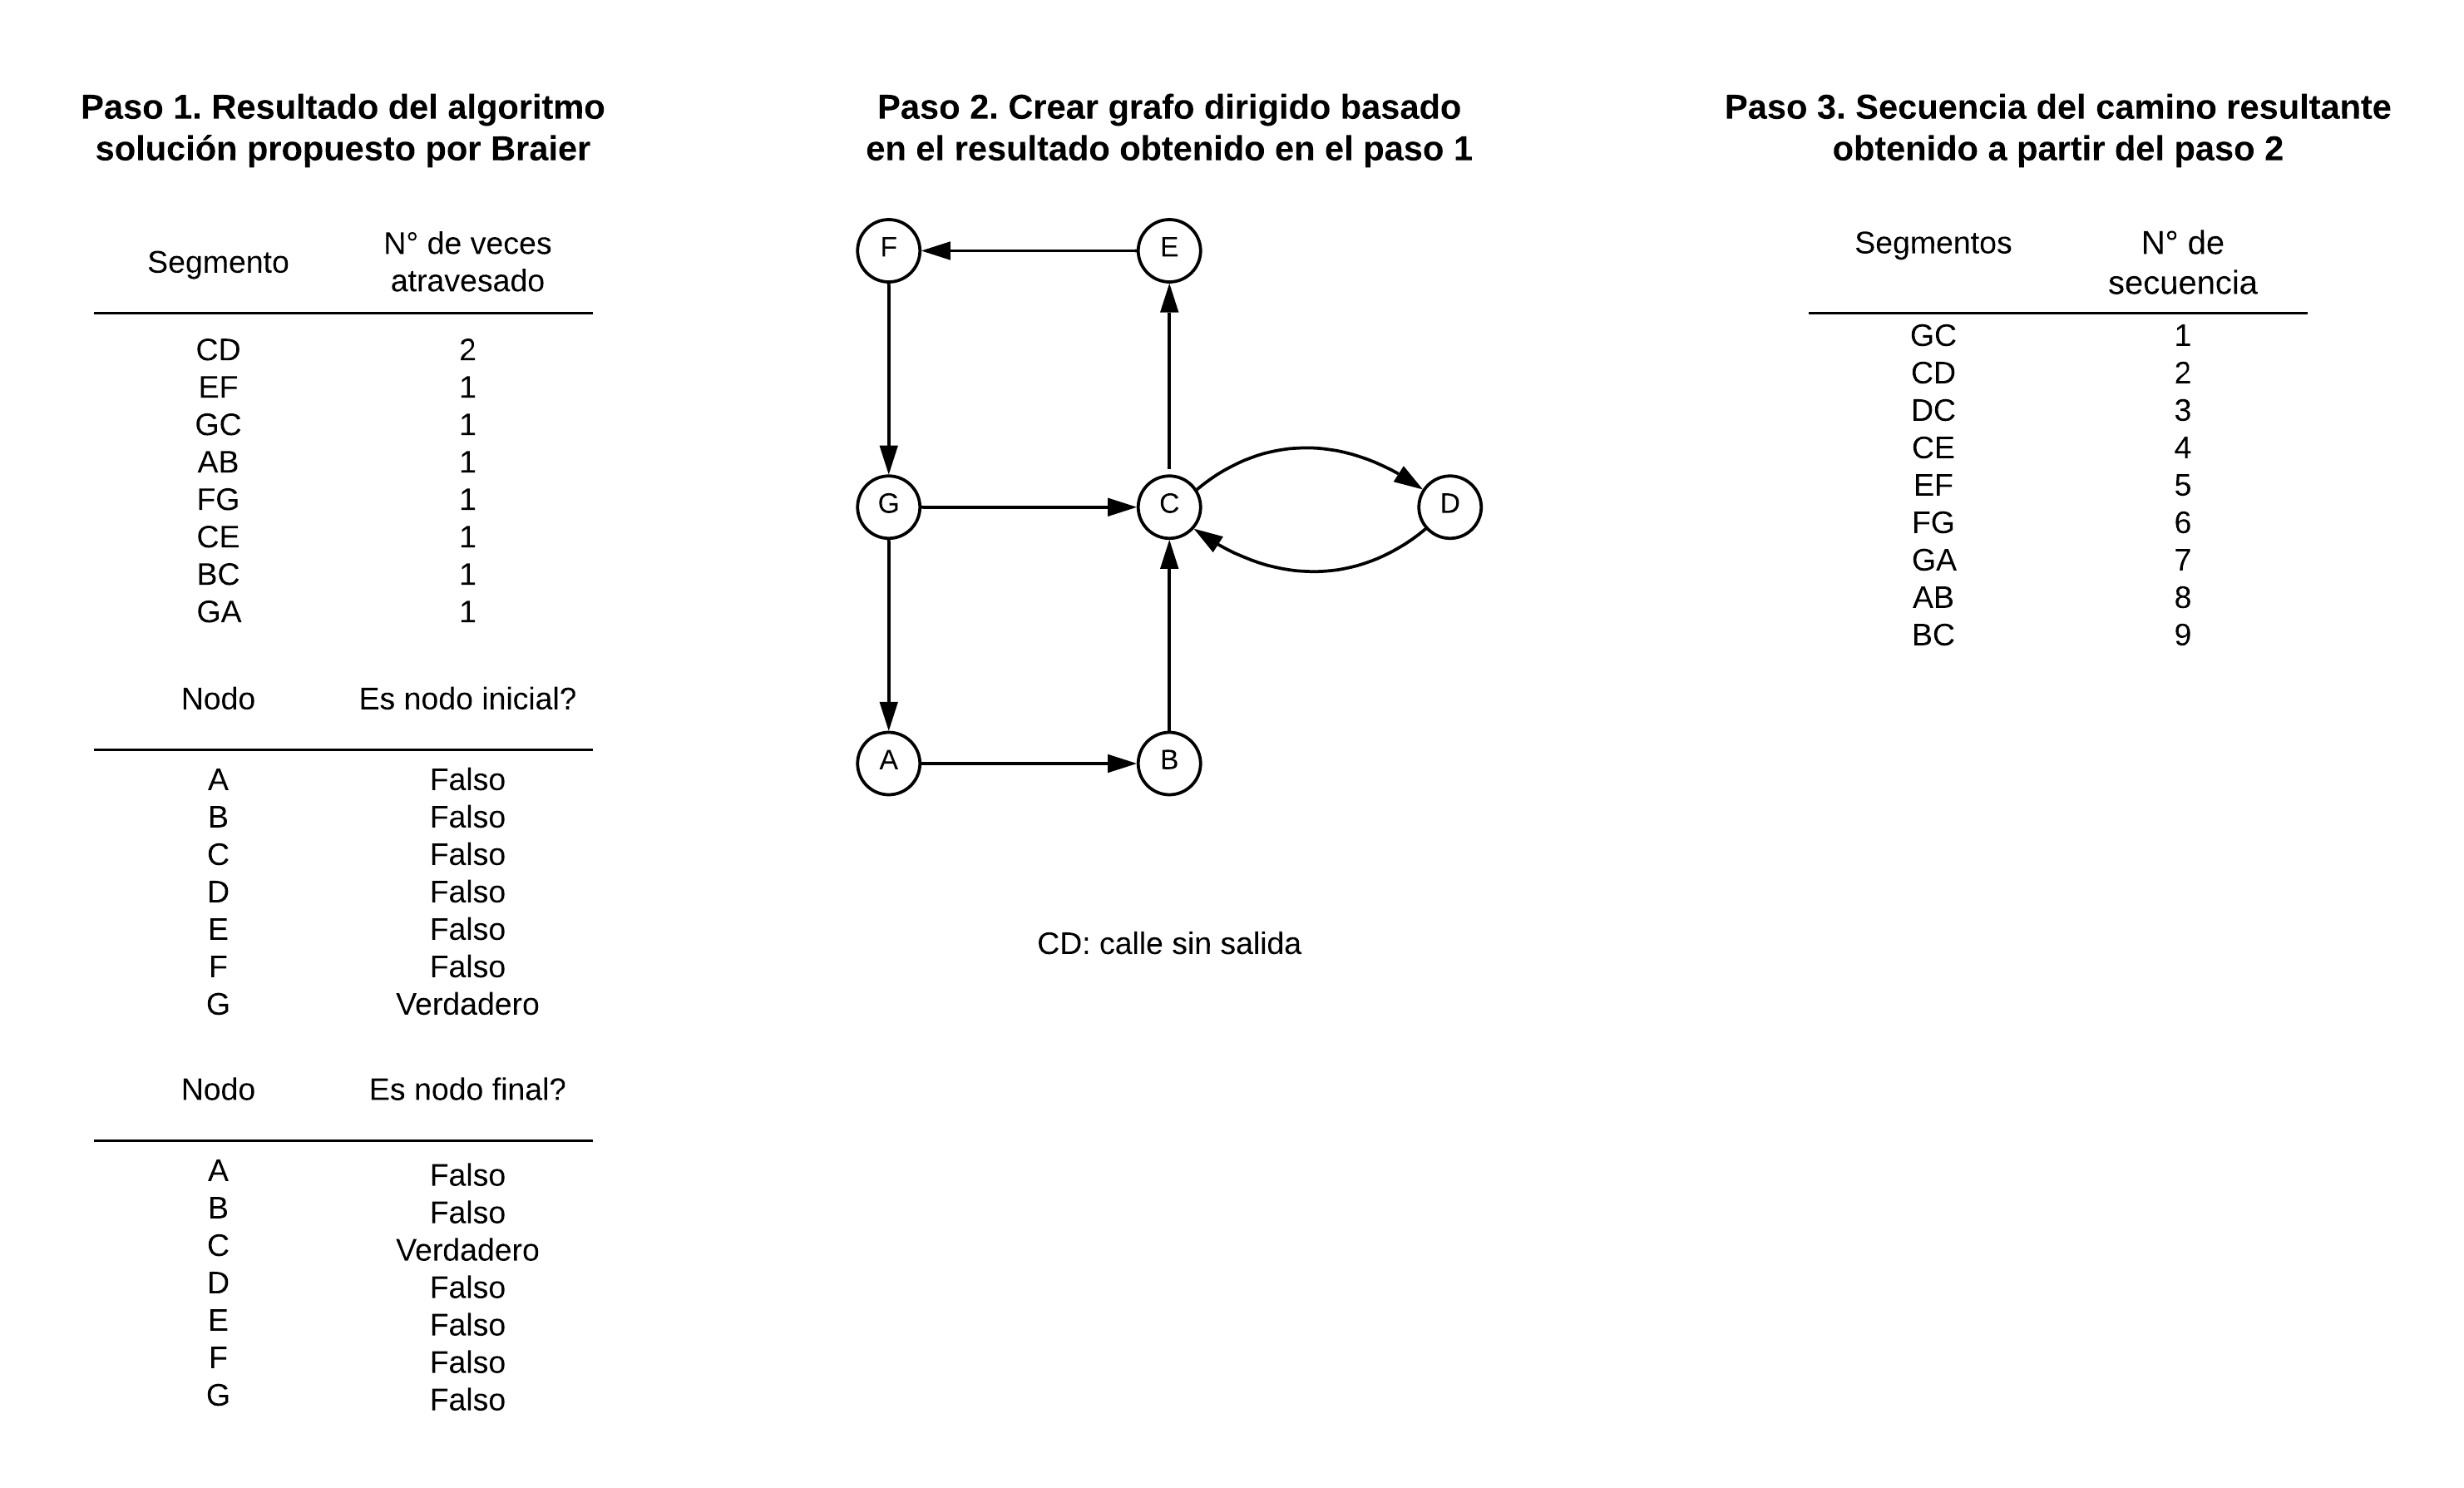
\includegraphics[width=\textwidth]{pasos_de_solucion.png}}
\caption{Pasos de solución para obtener la secuencia del camino del vehículo recolector en una zona.}
\label{fig:PasosSolucion}
\end{figure}


 % Planteamiento del problema

\clearpage
\lhead{\emph{Aplicación TapeYty}} 
\renewcommand\chaptername{Capítulo}%título "Capítulo"
\chapter{Aplicación TapeYty}
\label{solucionpropuesta}
\ifpdf
  \graphicspath{{Chapter6/Chapter6Figs/PNG/}{Chapter6/Chapter6Figs/PDF/}{Chapter6/Chapter6Figs/}}
\else
  \graphicspath{{Chapter6/Chapter6Figs/EPS/}{Chapter6/Chapter6Figs/}}
\fi

\markboth{\hfill \thechapter. Aplicación \textit{TapeYty}}{\hfill \thechapter. Aplicación \textit{TapeYty}}

En la actualidad, la DSU no cuenta con un \textit{software} que apoye a la toma de decisiones en lo que respecta a la gestión de residuos sólidos urbanos, más específicamente en el área de recolección. Por lo tanto, se propone la implementación de una herramienta GIS que contribuya con la elección de mejores caminos a seguir por los vehículos recolectores, y de esta manera generar mayores beneficios en cuanto a tiempo y distancia, además de garantizar que el servicio sea brindado a todos los domicilios.
%además de contribuir con el cuidado del medio ambiente.

La implementación consta de los siguientes módulos:
\begin{enumerate}
    \item Seguridad: El sistema comprende un mecanismo de autenticación basada en tokens JWT (\textit{JSON Web Tokens}). Se restringe acceso a la aplicación y a los servicios web REST del servidor no autenticados.
    \item Administración: Comprende la gestión (listar, agregar, editar, eliminar) de usuarios y vehículos.
    \item GIS: Este módulo despliega el mapa con las diferentes capas (zona, calle, departamento, distrito) y permite el manejo de capas, la gestión de calles, generación de rutas, despliegue de resultado de ruta optimizada.
    %(Ver Figura \ref{fig:aplicacionRutas}).
\end{enumerate}

\section{Arquitectura de aplicación}

La Figura \ref{fig:disenhoArquitectura} muestra el diseño de la arquitectura de \textit{software} alrededor de la aplicación solución \textit{TapeYty}. Este diseño se divide en dos partes que se explicarán en detalle a continuación.

\begin{figure}[bp]
\centerline{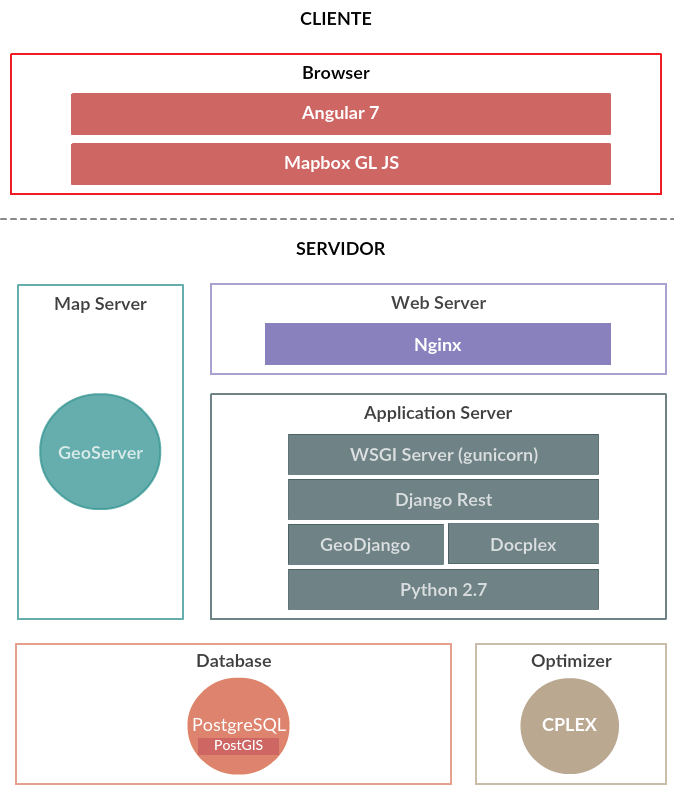
\includegraphics[width=\textwidth]{20190424_WebAppArchitectureDesign.png}}
\caption{Diseño de arquitectura de \textit{TapeYty}.}
\label{fig:disenhoArquitectura}
\end{figure}

\subsection{Cliente}

Desde una computadora portátil o un teléfono móvil el usuario puede acceder a la aplicación e ingresar con sus credenciales desde el navegador (\textit{browser}). Se ejecuta en el navegador el código Javascript generado a partir del código fuente construido con el marco (\textit{framework}) Angular (en su versión 7.0). Angular es un \textit{framework} ampliamente utilizado para el desarrollo de aplicaciones web con excelentes prestaciones en cuanto a rendimiento, escalabilidad, velocidad de respuesta y no menos importante una comunidad numerosa y activa. 

Una de las librerías incorporadas al proyecto cliente (\textit{frontend}) más relevantes es Mapbox GL JS, la cual ofrece funcionalidades relacionadas a mapas, teniendo como gran atractivo su buen desempeño durante el tiempo de renderizado de los mapas y datos geográficos.
% Utiliza WebGL, es una especificacion estandar que define una API javascript para la renderizacion de graficos en 3D dentro de cualquier navegador web. Aprovecha mejor la GPU(Unidad de procesamiento gráfico) desde cualquier navegador (web) que soporte OpenGL 2.0 o mayor.

\subsection{Servidor}

El lado servidor presenta mayor complejidad ya que concentra varios componentes que además deben interactuar unos con otros.

Como parte de la solución, se utiliza el gestor de base de datos relacional PostgreSQL (versión 10.8) con su extensión PostGIS (version 2.4), donde están almacenadas las distintas informaciones obtenidas, geográficas o no, excepto los datos (\textit{shapes}) que provienen del SNC de Paraguay.

Los mapas bases de Departamentos y Distritos del SNC son almacenados en el servidor de mapas Geoserver que se muestra en la Figura \ref{fig:disenhoArquitectura}. También se crea una conexión con la base de datos para poner a disposición las capas o mapas de calles y zonas, en modo lectura, donde el servidor ofrece servicios web de mapas TMS (\textit{Tile Map Service}), servicio que maneja estrategias de caché de cuadros de imágenes para mostrar los mapas con mayor velocidad dando un mejor rendimiento a la aplicación.

% El servidor de mapas GeoServer consiste en un servidor de código abierto escrito en Java que permite a los usuarios compartir y editar datos espaciales. En este servidor se almacenan los mapas bases de Departamentos y Distritos del Catastro Nacional. Además, se crea una conexión con la base de datos para poner a disposición las capas o mapas de calles y zonas, en modo lectura, donde el servidor ofrece servicios web de mapas como por ejemplo \textit{TMS} (\textit{Tile Map Service}), servicio que maneja estrategias de caché de cuadros de imágenes para mostrar los mapas con mayor velocidad dando un mejor rendimiento a la aplicación.

Para resolver el modelo matemático seleccionado se requiere de un \textit{software} especializado para ello. Se opta por la herramienta \textit{CPLEX Optimizer} de IBM \citep{CPLEXOptimizer} en su versión académica 12.8, ya utilizado en trabajos previos \citep{Vecchi2016ACollection,Ramos2018TheApproaches,BabaeeTirkolaee2019DevelopingStudy}. El modelo matemático puede ser codificado en CPLEX con el lenguaje OPL ({\textit{Optimization Programming Language}}), provee además interfaces C, C++, Java y Python para su modelado. Sin embargo, estas interfaces no son usadas directamente para modelar sino a través de la librería Docplex \citep{Docplex} detallada más adelante.

Para el desarrollo propio de una aplicación web una de las preocupaciones más importantes es la elección del lenguaje y el framework sobre los cuales estará construida. En este trabajo se opta por el lenguaje Python, conjuntamente con el framework GIS GeoDjango. En el área GIS, Python es uno de los lenguajes más utilizados a lo largo del tiempo, pudiéndose encontrar muchas funciones, librerías, \textit{software}, entre otros; escritos con este lenguaje. GeoDjango, basado en Django, tiene la virtud de ser robusto, provee un modelo de programación MVC (\textit{Model-View-Controller}) y facilita el desarrollo de aplicaciones Web.

La librería Docplex de Python resulta en una sencilla integración con nuestro \textit{framework}, también permite formular el modelo de forma clara y directa en comparación con las interfaces de CPLEX, resultando muy similar a la formulación con el lenguaje OPL (Ver Algoritmo \ref{codigoDocplex}).

\hfill
\begin{lstlisting}[language=Python,caption={Fragmento de código en docplex.},label={codigoDocplex}]
from docplex.mp.model import Model

# ************************ INSTANCIA DEL MODELO ******************************

moron_model = Model(name='moron')
    
# ************************* VARIABLES DE DECISION ****************************

s = {i: moron_model.binary_var(name='s_{0}_{1}'.
    format(i.gis_nodo.gis_nodo_id, i.nodo_expandido_id)) 
    for i in iniciales}
t = {t: moron_model.binary_var(name='t_{0}_{1}'.
    format(t.gis_nodo.gis_nodo_id, t.nodo_expandido_id)) 
    for t in nodos_expandidos}

# **************************FUNCION OBJETIVO *********************************
moron_model.minimize(
    moron_model.sum(x[a.nodo_expandido_origen, a.nodo_expandido_destino] * a.peso 
    for a in arcos_expandidos))
    
# **************************** RESTRICCIONES *********************************
# Garantizan que el nodo inicial sea unico
moron_model.add_constraint(moron_model.sum(s[i] for i in iniciales) == 1)

# Garantizan que el nodo final sea unico
moron_model.add_constraint(moron_model.sum(t[i] for i in nodos_expandidos) == 1))
\end{lstlisting}

Con Docplex y GeoDjango se implementa toda la lógica de negocio de la aplicación. Para poder acceder a esta lógica desde el cliente se brinda una API (\textit{Application Programming Interface}). Para ello, se utiliza el protocolo de comunicación de intercambio de datos RESTful con la librería Django REST Framework y Django Rest Framework GIS. Se implementan los servicios para los módulos citados anteriormente como: agregar, eliminar y editar usuarios, editar propiedades alfanuméricas de calles, generar la ruta óptima de una zona, entre muchos otros; con estructuras de datos en formato JSON (\textit{JavaScript Object Notation}) y geoJSON.

Con esto la aplicación está prácticamente lista, queda preparar el ambiente de producción para su implantación. Se instala uno de los servidores web más comunes actualmente, Nginx. El servidor web recibe una solicitud HTTP del cliente (el navegador), interpreta la solicitud y la envía a la puerta de enlace (\textit{gateway}). El \textit{gateway} Gunicorn es un servidor HTTP de Interfaz de Pasarela del Servidor Web de Python (WSGI, \textit{Web Server Gateway Interface}) que traduce la solicitud recibida del servidor web para que la aplicación pueda manejarlo. Y por el último tenemos la aplicación servidor que a través de su API Rest recibe la petición para luego procesarla y responderla.

\section{Aplicación}

En esta sección se detallarán las principales funcionalidades que constituyen la aplicación \textit{TapeYty}. En el Apéndice \ref{sec:manual-usuario} se encuentra disponible el manual de usuario donde se detalla la totalidad de las funcionalidades del sistema.

\subsection{Modelo de datos}

La Figura \ref{fig:DERTapeYty} muestra el modelado de datos a partir de un Diagrama Entidad-Relación (DER), diseñado con la herramienta SQLPowerArchitect \citep{SQLArchitect} en su versión 1.0.8. A continuación, en la Tabla \ref{tab:descripcionDER} se detalla brevemente cada tabla en el DER.

\begin{landscape}
\begin{figure*}[tbp]
\centerline{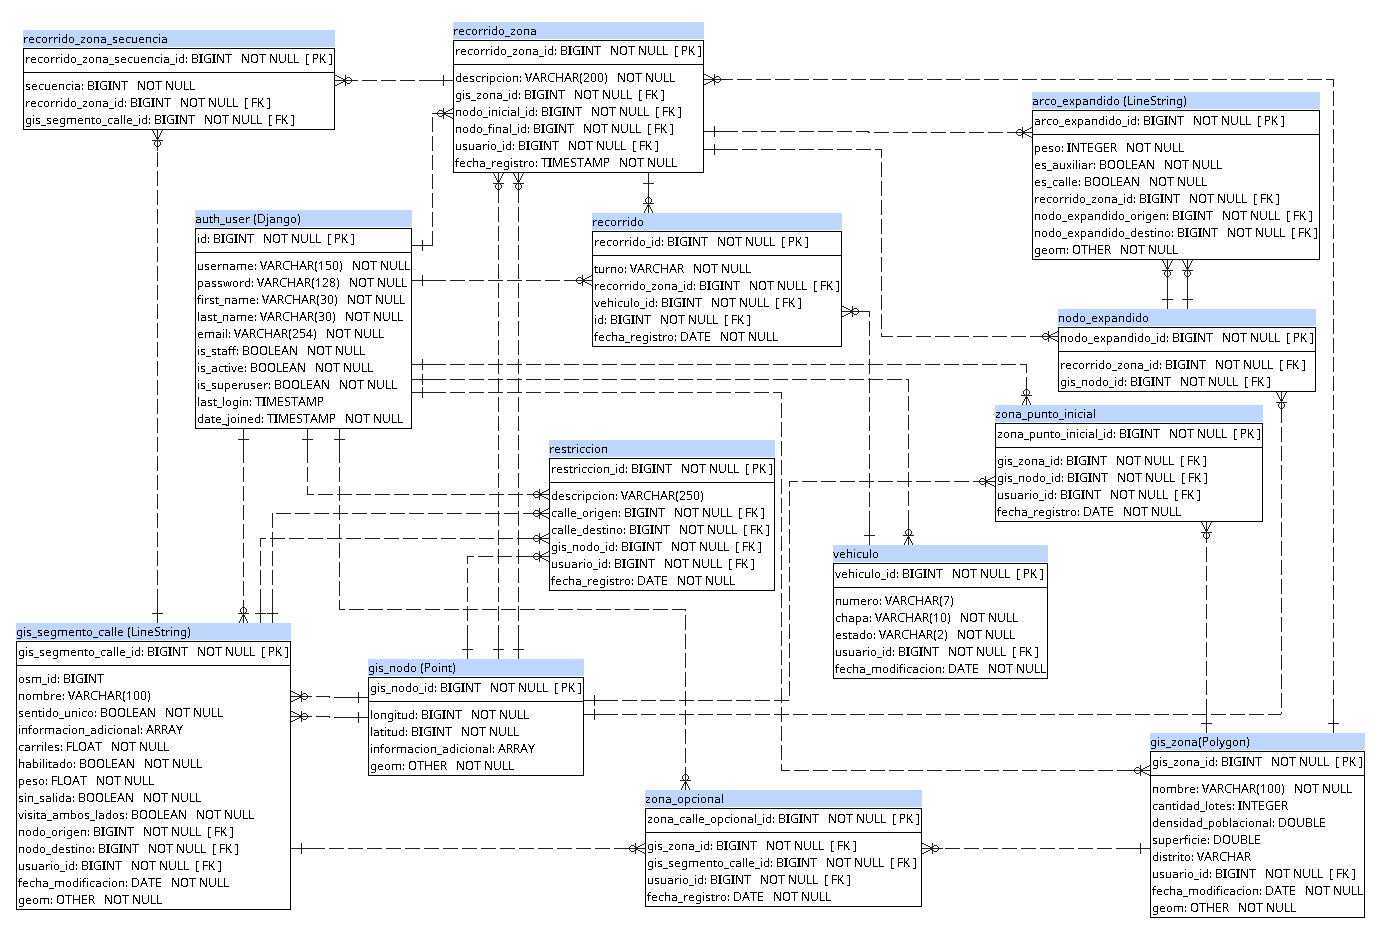
\includegraphics[height=\textheight]{20190716_DER.png}}
\caption{Diagrama Entidad-Relación de \textit{TapeYty}.}
\label{fig:DERTapeYty}
\end{figure*}
\end{landscape}

% Please add the following required packages to your document preamble:
% \usepackage{multirow}
% \usepackage{graphicx}
\begin{table}[]
\caption{Descripción del modelo de datos de \textit{TapeYty}.}
\label{tab:descripcionDER}
\resizebox{\textwidth}{!}{%
\begin{tabular}{lll}
\hline
Uso                                                                                              & Nombre de tabla            & Descripción                                                                                                                                                        \\ \hline
\begin{tabular}[c]{@{}l@{}}Autenticación y \\ auditoría\end{tabular}                             & auth\_user                 & \begin{tabular}[c]{@{}l@{}}Creada por Django, es referenciada en todas las tablas que \\ pueden ser editadas por el usuario en la aplicación \textit{TapeYty}.\end{tabular} \\ \hline
\multirow{3}{*}{Capas}                                                                           & gis\_nodo                  & \begin{tabular}[c]{@{}l@{}}Representan puntos en el mapa. Los datos iniciales son \\ cargados desde OSM.\end{tabular}                                              \\
                                                                                                 & gis\_segmento\_calle       & \begin{tabular}[c]{@{}l@{}}Representan segmentos de calle en el mapa. Los datos \\ iniciales son cargados desde OSM.\end{tabular}                                  \\
                                                                                                 & gis\_zona                  & \begin{tabular}[c]{@{}l@{}}Representan las zonas de trabajo del departamento de\\ recolección de la DSU.\end{tabular}                                              \\ \hline
\multirow{3}{*}{\begin{tabular}[c]{@{}l@{}}Lógica de recolección\\ DSU\end{tabular}}             & zona\_calle\_opcional      & \begin{tabular}[c]{@{}l@{}}Representan las calles dentro o en el límite de una zona \\ que pueden no ser recorridos por el vehículo recolector.\end{tabular}       \\
                                                                                                 & zona\_punto\_incial        & \begin{tabular}[c]{@{}l@{}}Representan puntos en el límite de una zona en donde \\ se puede empezar el reccorrido.\end{tabular}                                    \\
                                                                                                 & restriccion                & Representan prohibiciones de giro y contramano.                                                                                                                    \\ \hline
\multirow{2}{*}{\begin{tabular}[c]{@{}l@{}}Representación del \\ grafo $G'$\end{tabular}} & nodo\_expandido            & Representa el conjunto $V$ del modelado.                                                                                                                             \\
                                                                                                 & arco\_expandido            & Representa el conjunto $A$ del modelado.                                                                                                                             \\ \hline
\multirow{4}{*}{Recorrido}                                                                       & vehiculo                   & Representa un vehículo de la DSU.                                                                                                                                  \\
                                                                                                 & recorrido                  & El recorrido es asociado a un vehículo y turno de la DSU.                                                                                                          \\
                                                                                                 & recorrido\_zona            & Cada recorrido es asociado a una zona.                                                                                                                             \\
                                                                                                 & recorrido\_zona\_secuencia & Representa la secuencia de un recorrido en una zona.                                                                                                               \\ \hline
\end{tabular}%
}
\end{table}

\subsection{Funcionalidades más relevantes}

\subsubsection{Editar un segmento de calle}

El sistema permite modificar propiedades (no geométricas) de los segmentos de calles. En la Figura \ref{fig:edicionCalles} se selecciona un segmento de la calle General Bernardino Caballero indicado con un color amarillo y con sus puntos extremos pintados.

En el panel derecho de la aplicación se muestra el sentido del segmento, el punto de color rosa claro representa en el mapa el origen del trayecto a seguir mientras que el punto lila indica su destino. Además, se observa que el segmento de calle se encuentra habilitado para su circulación. El usuario puede modificar el sentido del segmento invirtiendo el origen y destino, convertir el segmento a uno de doble sentido y deshabilitar el segmento de calle para su circulación. Los segmentos de calles deshabilitados no forman parte de las rutas generadas.
 
Es importante mencionar que un cambio en las propiedades de un segmento puede generar inconsistencias en la red de calles, y consecuentemente, produzca un resultado infactible en la generación de la ruta optimizada. Por ejemplo, si un segmento de calle sin salida habilitado se establece como de único sentido, no se podrá acceder o salir del mismo impidiéndose que se cumplan las restricciones de conservación de flujo del modelo.

\begin{figure}[H]
\centerline{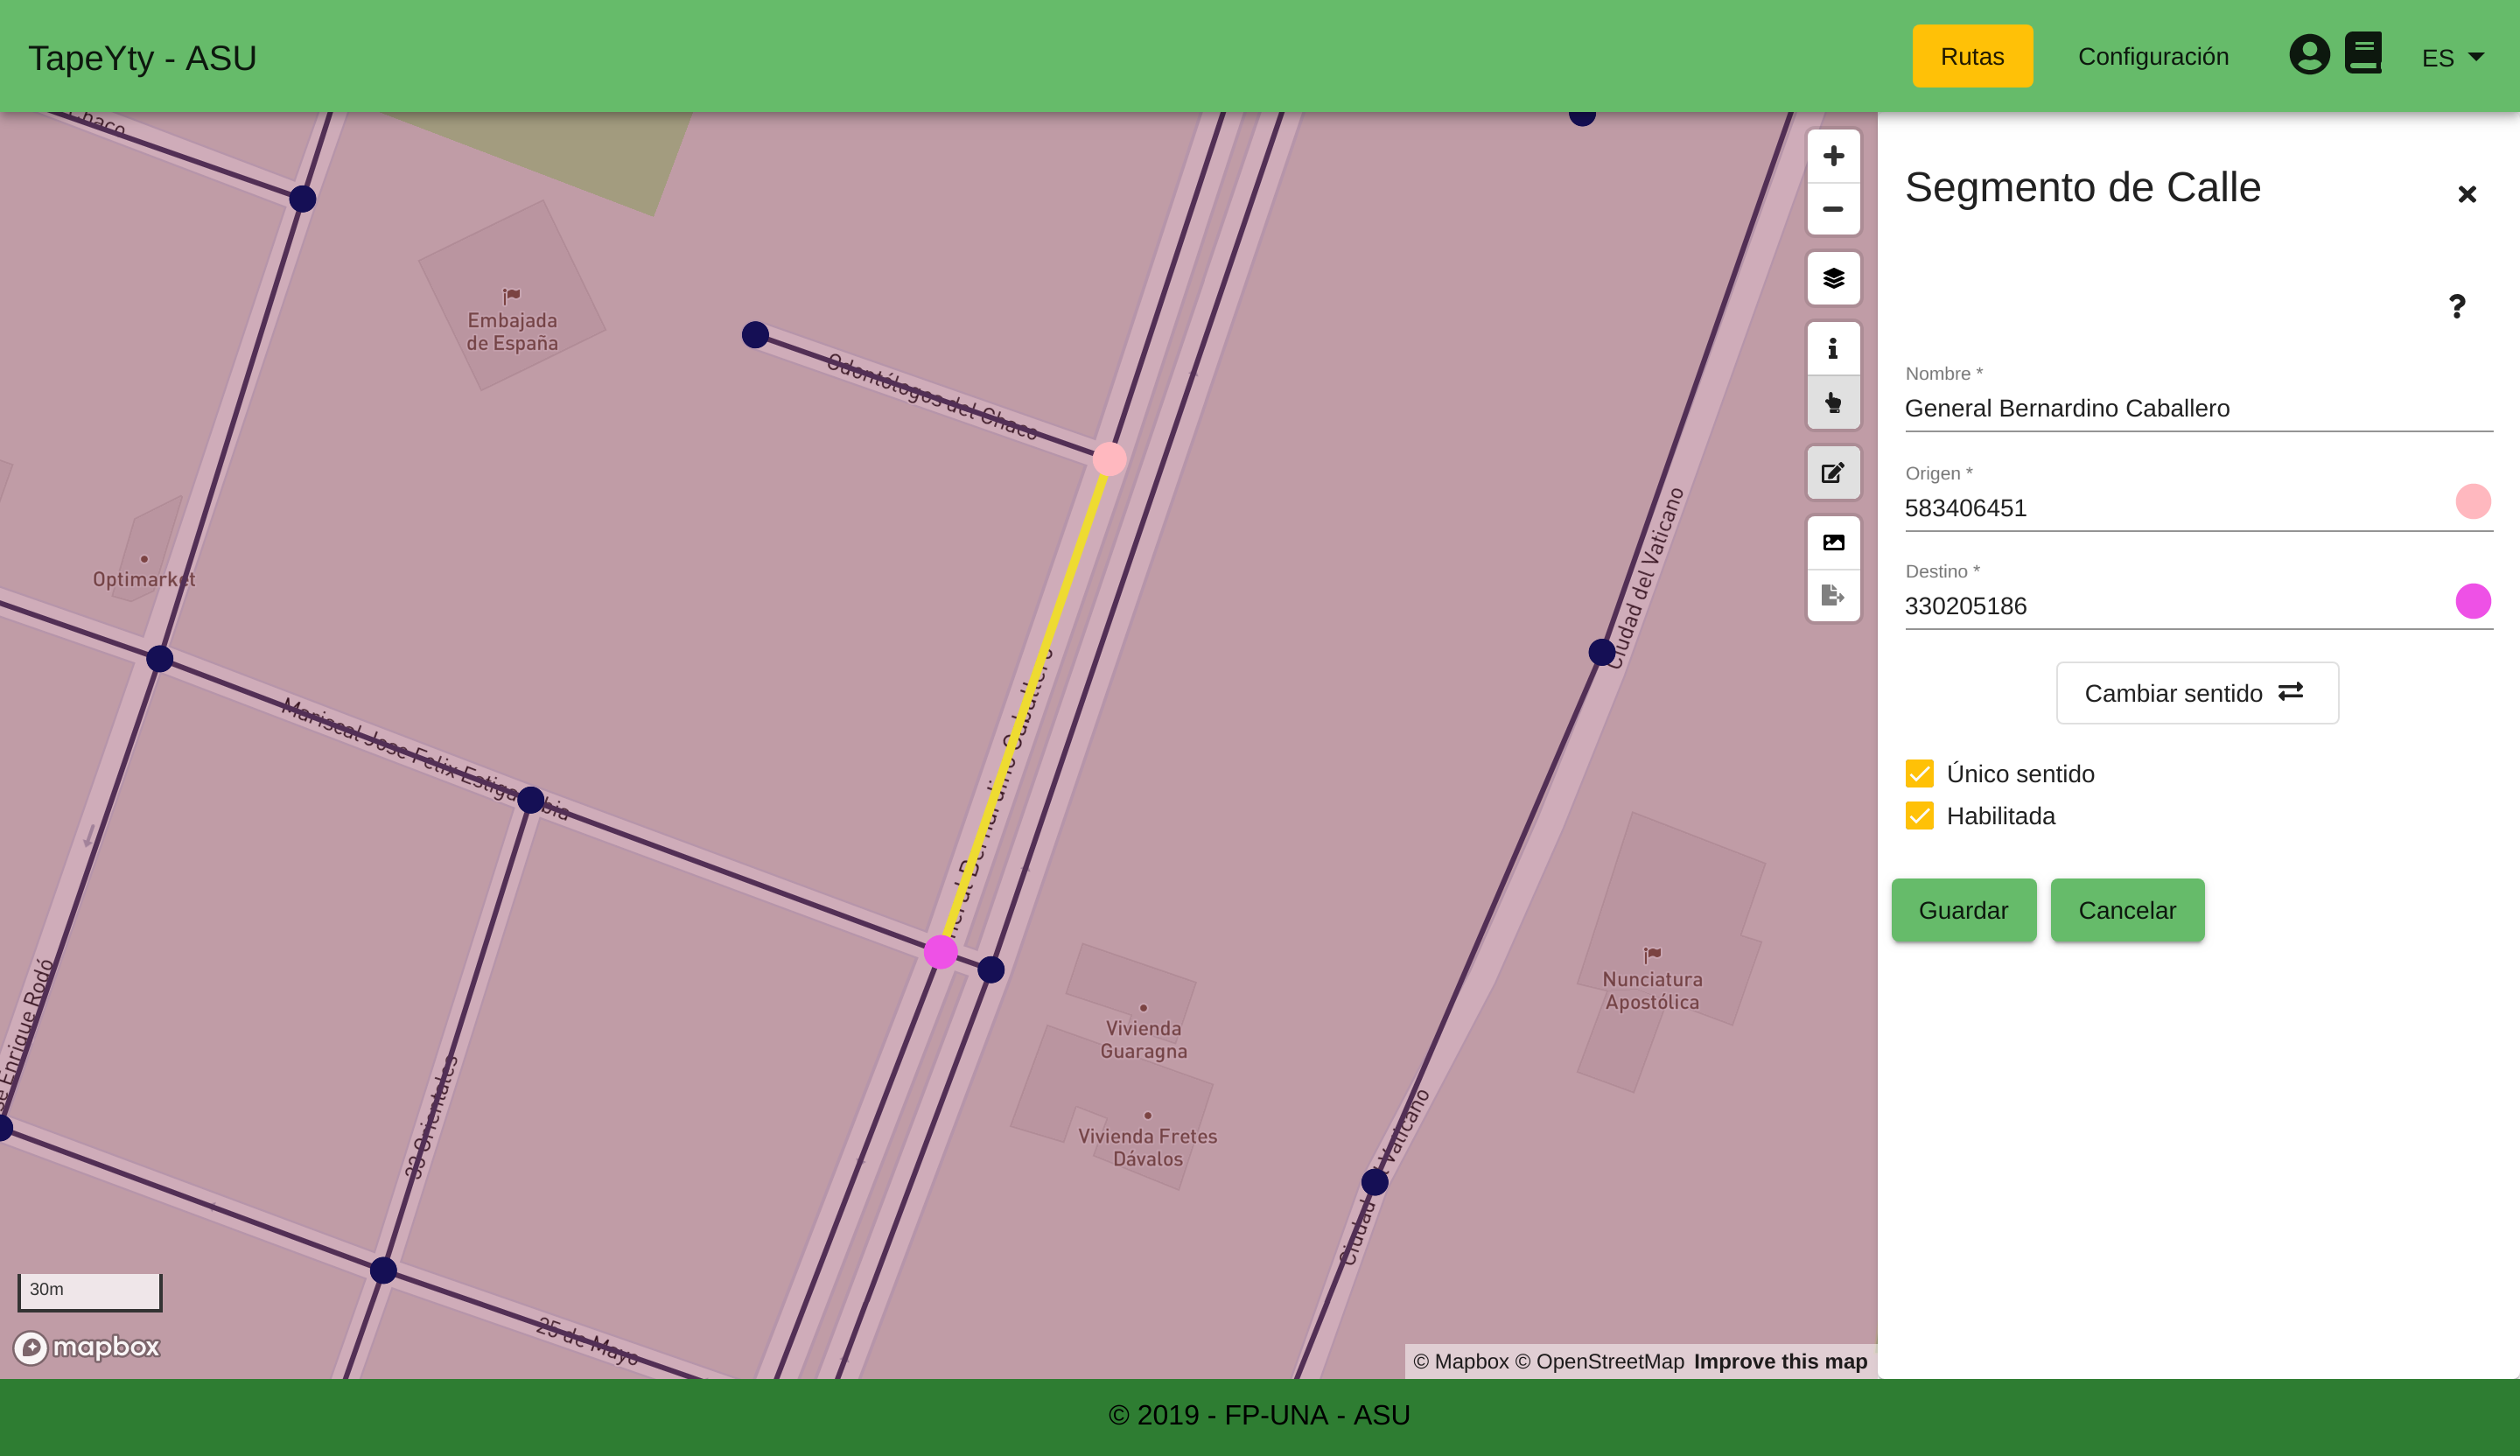
\includegraphics[width=\textwidth]{edicionCalle.png}}
\caption{Edición de un segmento de calle en \textit{TapeYty}.}
\label{fig:edicionCalles}
\end{figure}

\subsubsection{Agregar calles opcionales para el recorrido de una zona}

% Para poder establecer si las calles que se encuentran en el límite de una zona pertenecen o no a la zona en cuestión en el sistema se definen las calles opcionales de una zona. 
En la Figura \ref{fig:callesOpcionales} se observan que los segmentos de las Avenidas Kubitschek, Mariscal López y General Santos que limitan la zona seleccionada se encuentran resaltadas en color verde, indicándose como opcionales, es decir, en el modelo se establece que estos segmentos no requieren ser atravesados para su respectiva recolección.

Una vez que el usuario selecciona la opción de agregar o eliminar los segmentos de calle opcionales de una zona, se despliegan los segmentos de calles que se encuentran cubiertos por la zona seleccionada utilizando la función \textit{coveredby} de Django que es equivalente a la función \textit{ST\_CoveredBy} en PostGIS.

\begin{figure}[H]
\centerline{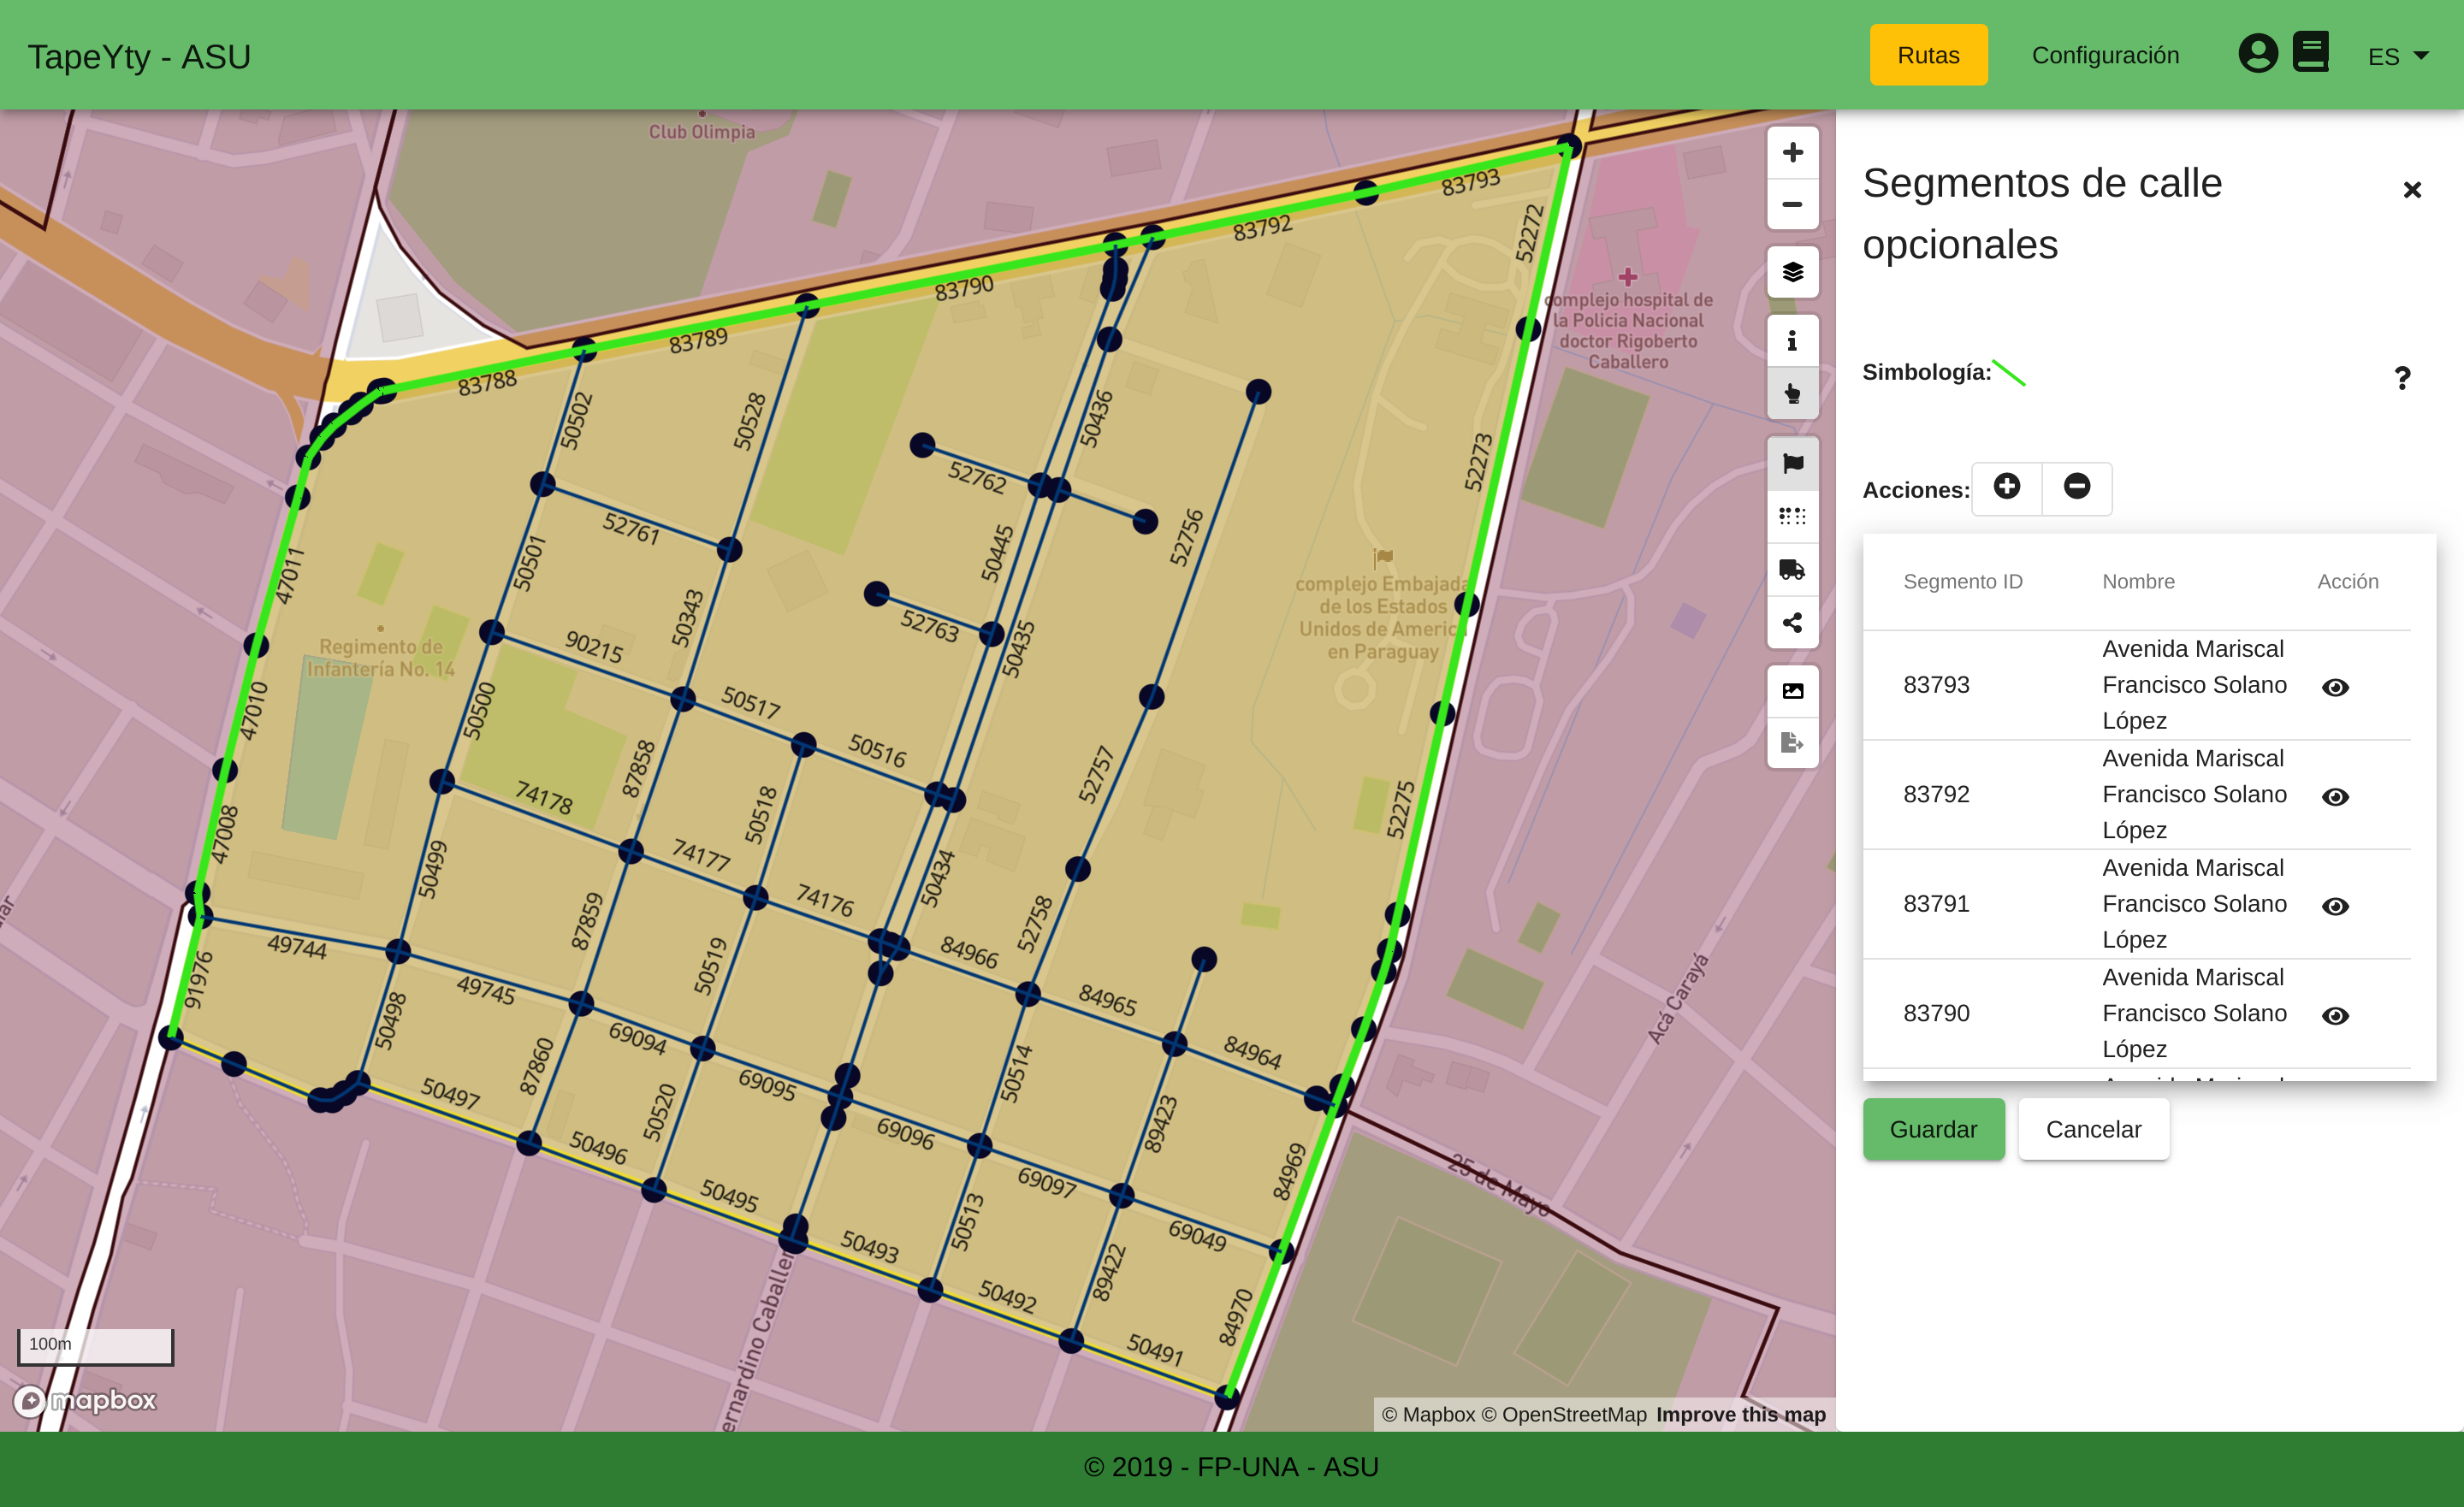
\includegraphics[width=\textwidth]{callesOpcionales.png}}
\caption{Agregar o eliminar calles opcionales de una zona en \textit{TapeYty}.}
\label{fig:callesOpcionales}
\end{figure}

\subsubsection{Agregar posibles puntos iniciales para el recorrido de una zona}

El conductor del camión recolector en el inicio de su recorrido dentro de una zona deberá atravesar primeramente una de las calles que conforman el límite de dicha zona. Los nodos o puntos extremos de los segmentos que forman parte de estos límites, por ende, conforman los posibles puntos iniciales del recorrido y a su vez corresponden a los datos de entrada del modelo. 

En la mayoría de los casos, es probable que el camión ingrese por alguno de los puntos más cercanos de hacia donde viene dirigido el conductor y no precisamente del otro extremo de la zona. Esto deriva en la necesidad de seleccionar no todos, sino más bien unos pocos puntos del borde de la zona como posibles inicio de la ruta óptima.

En la Figura \ref{fig:puntosIniciales} se observa en el mapa en color verde los posibles puntos de inicio para el camino a seguir. En el panel se despliega la lista de dichos puntos y también se tiene la posibilidad de editar la lista, agregando o eliminando puntos.

\begin{figure}[H]
\centerline{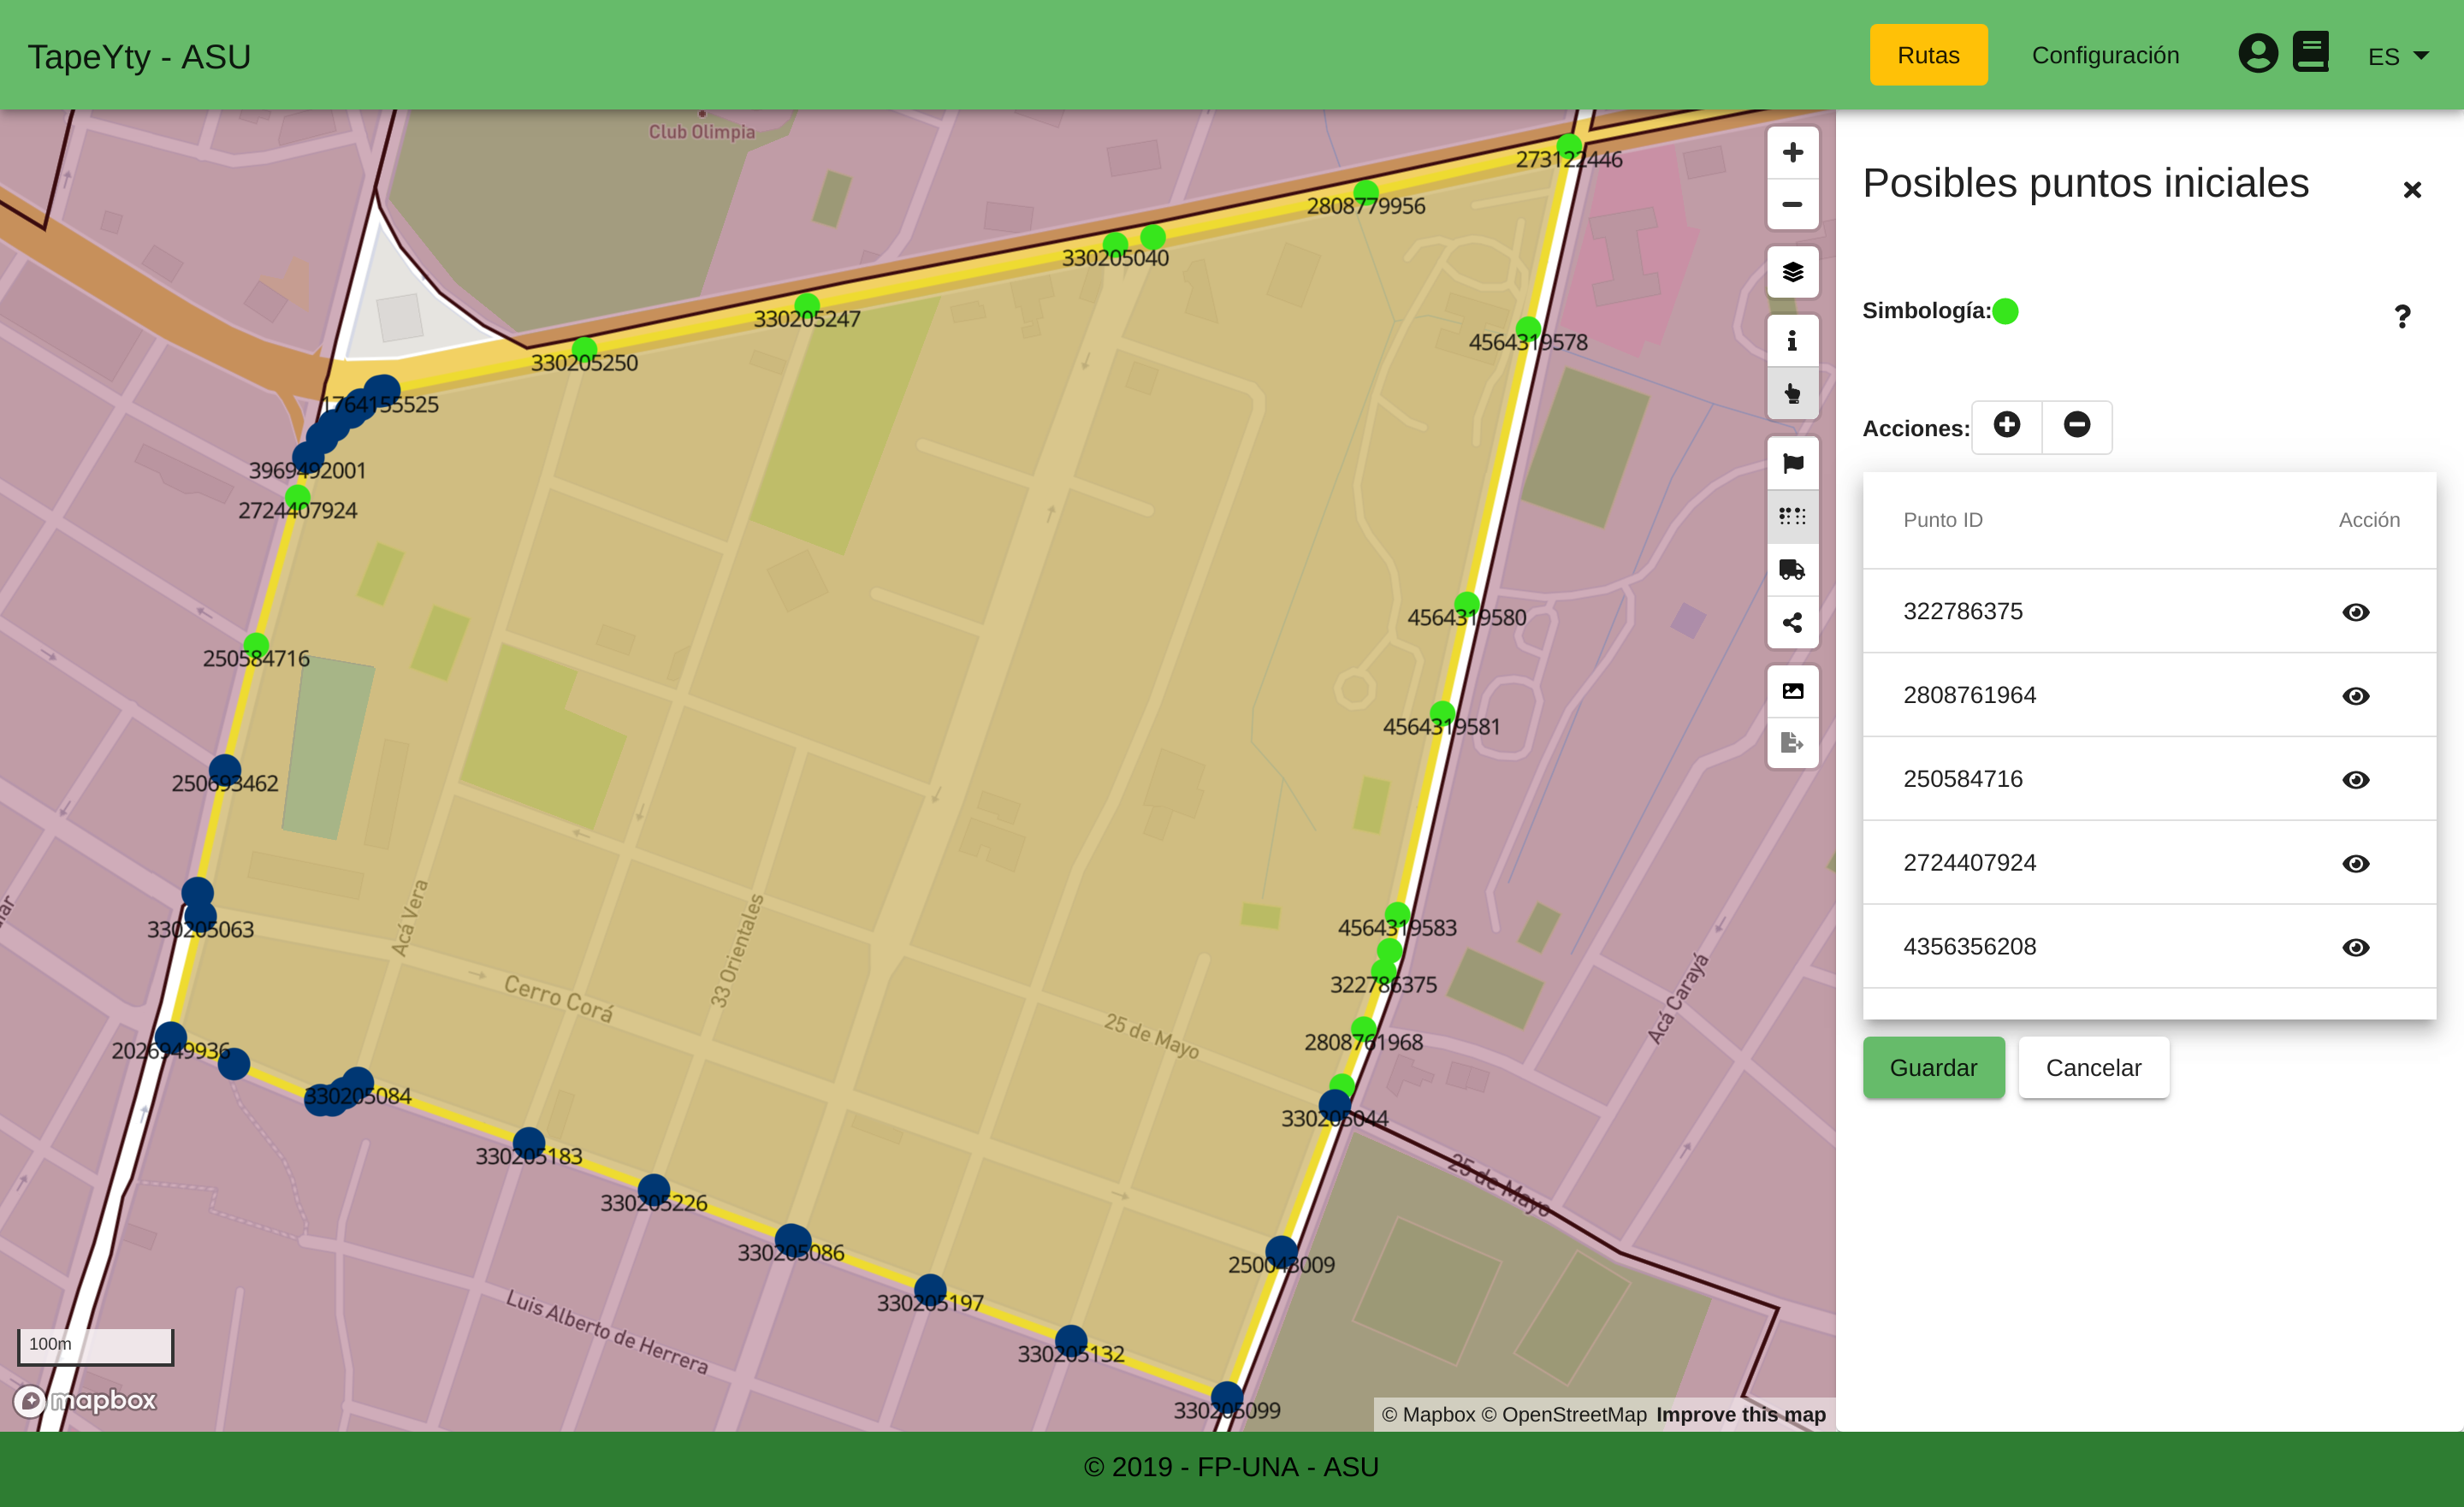
\includegraphics[width=\textwidth]{puntosIniciales.png}}
\caption{Agregar o eliminar posibles puntos de inicio de una zona en \textit{TapeYty}.}
\label{fig:puntosIniciales}
\end{figure}

\subsubsection{Agregar restricciones de red de ruta}

Para poder manejar correctamente las restricciones de la red de calles, el sistema permite agregar y eliminar restricciones que existan entre dos segmentos de calles que tengan un punto en común. 

En la Figura \ref{fig:restriccion} en el panel a la derecha de la aplicación se listan todas las restricciones que se dibujan en el mapa, desde el listado se puede eliminar una restricción o se puede seleccionarla. Al seleccionarla se resalta la prohibición de giro a la derecha desde la calle 25 de Mayo hacia la calle 33 Orientales.

En el mapa de la Figura \ref{fig:restriccion} se observa en color verde las restricciones que existen sobre los segmentos de calles que pertenecen a la zona seleccionada, y además sobre las que se encuentran hasta 220 metros alrededor de la zona en cuestión, ya que para generar la ruta de recolección se tienen en cuenta las calles dentro de una zona como las que se encuentran en una una banda perimetral de 220 metros representadas como segmentos opcionales.

\begin{figure}[H]
\centerline{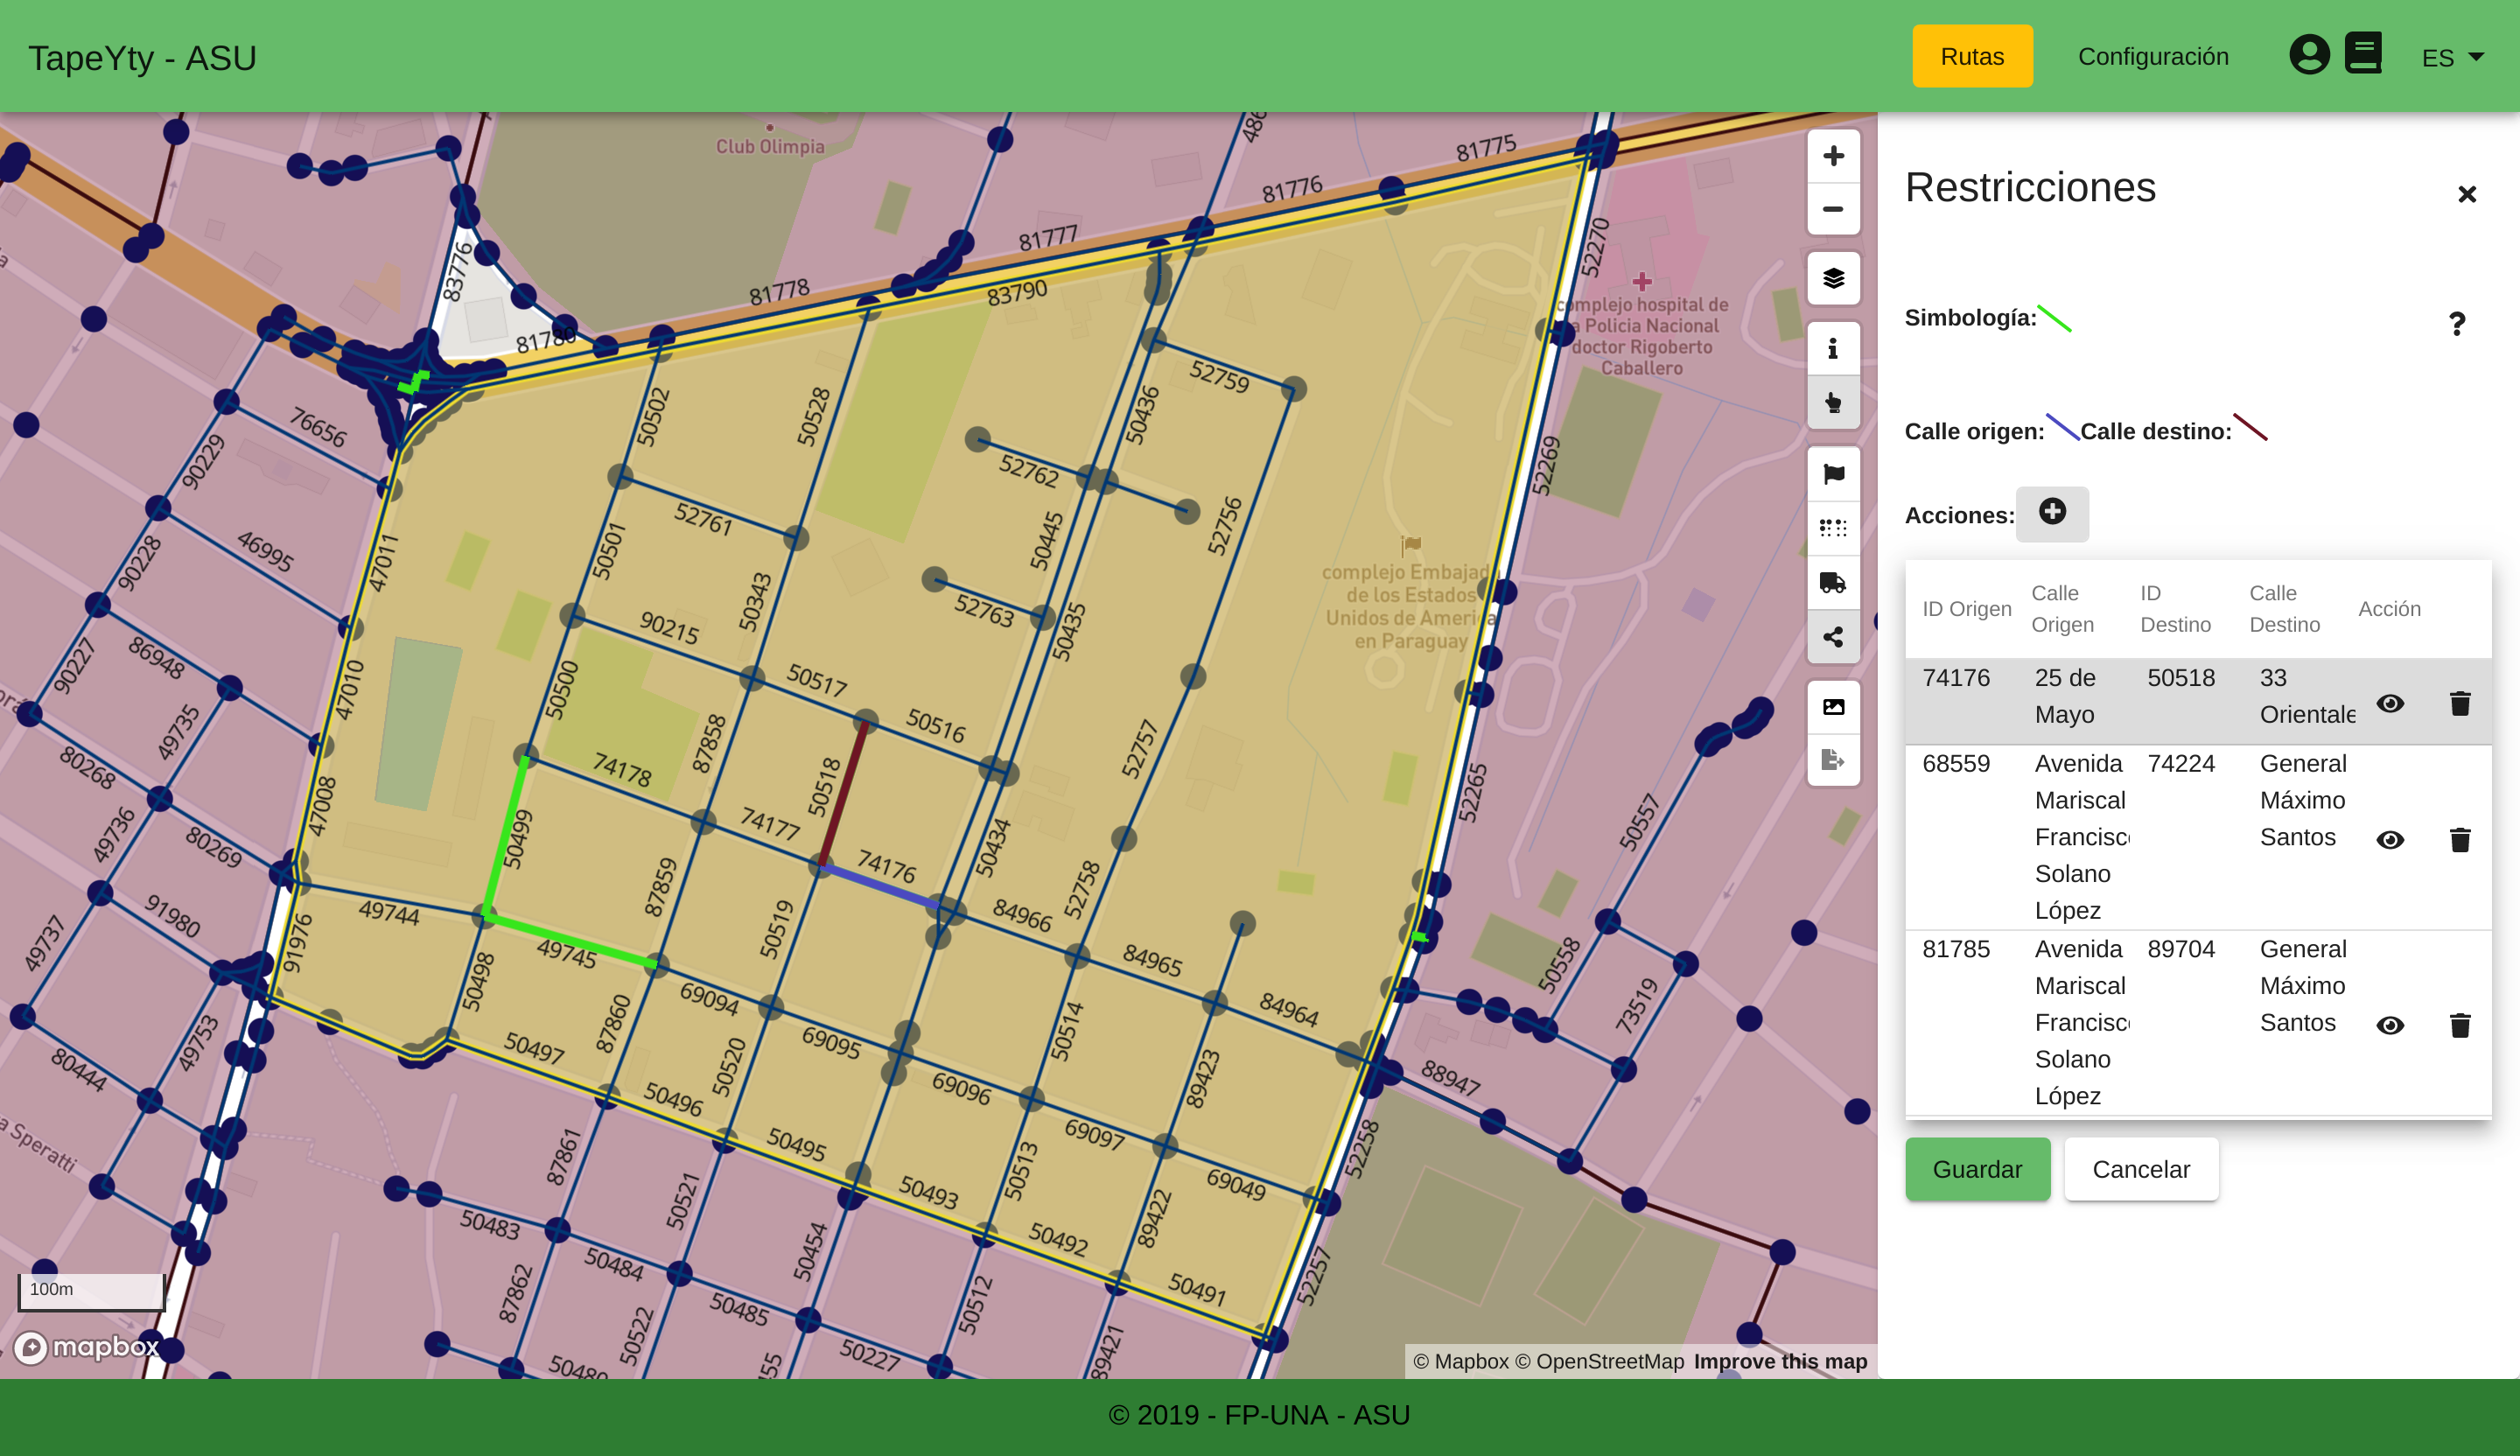
\includegraphics[width=\textwidth]{restricciones.png}}
\caption{Agregar o eliminar restricciones de giro y contramano en \textit{TapeYty}.}
\label{fig:restriccion}
\end{figure}

\subsubsection{Desplegar y descargar la ruta optimizada}

La Figura \ref{fig:generacionRuta} muestra finalmente como se despliega en el mapa la ruta óptima generada por el sistema. Se indican de forma clara los puntos inicial (color verde) y final (color rojo) del recorrido. Los segmentos contienen etiquetas que representan la secuencia en que deben ser visitados cada uno de ellos. Un segmento contiene una etiqueta con valores entre comas en el caso en que se pase más de una vez por el mismo segmento. Algunos valores de secuencia pueden no ser visibles a cierta escala por el simple hecho de evitar la superposición de etiquetas en segmentos contiguos. Para visualizarlos se debe realizar un acercamiento en el mapa desde la aplicación.

Es posible acceder al histórico de recorridos generados en una zona, buscarlos por alguna propiedad como nota o fecha para volver a desplegar uno de ellos en un momento dado. Se brinda además la opción de exportar el resultado y descargarlo como imagen en formato PNG y como archivo en formato GPX. El archivo GPX permite la navegación, por ejemplo, desde cualquier dispositivo GPS o a través de una aplicación del teléfono apropiada para ello como lo es ``Mi Ruta'' \citep{MiRuta}.

\begin{figure}[H]
\centerline{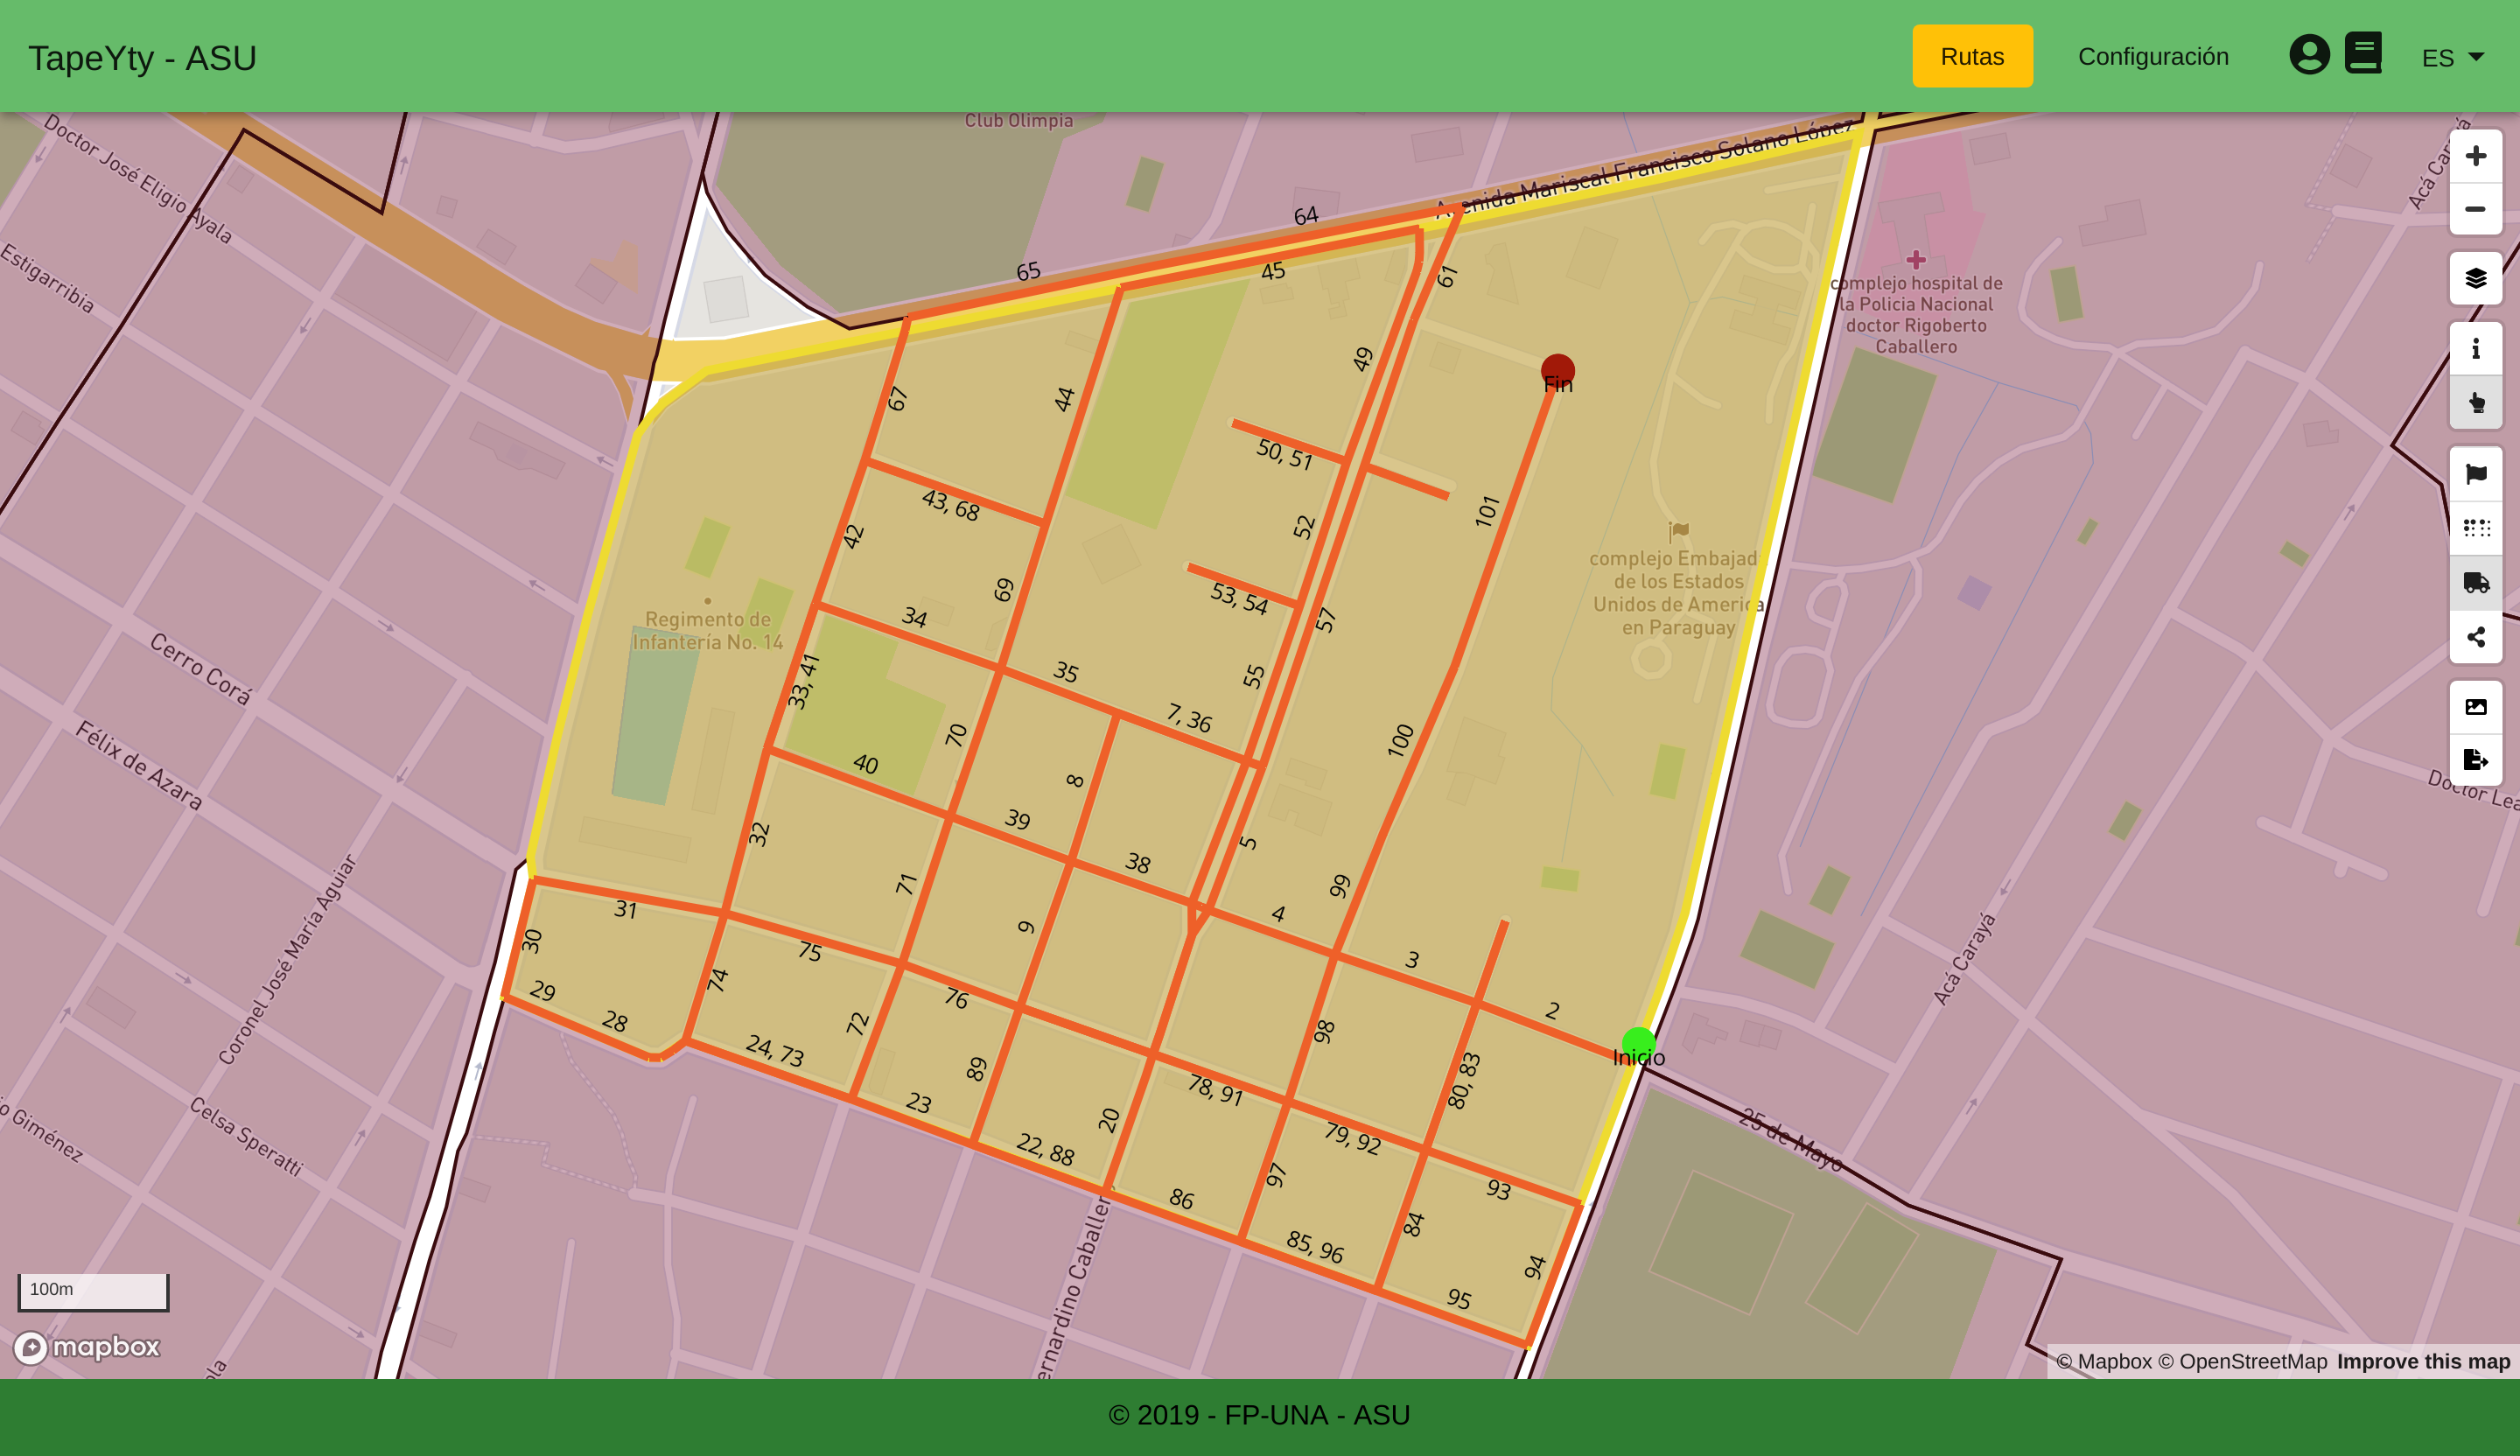
\includegraphics[width=\textwidth]{generacionRuta.png}}
\caption{Despliegue de ruta generada con \textit{TapeYty} en una zona de trabajo.}
\label{fig:generacionRuta}
\end{figure}


% Uno de los parámetros de entrada para el algoritmo, es el conjunto de los posibles puntos o nodos que podrán ser inicio del recorrido. A cada zona, lista de posibles nodos iniciales . Hablar con una imagen de la aplicación de dicha funcionalidad, de que si no se elige ninguno se realiza X operación GIS(ver Figura NN).

 % Solución propuesta

\clearpage
\lhead{\emph{Resultados y Discusión}} 
\renewcommand\chaptername{Capítulo}%título "Capítulo"
\chapter{Resultados y Discusión}
\label{resultadosdiscusion}
\ifpdf
  \graphicspath{{Chapter7/Chapter7Figs/PNG/}{Chapter7/Chapter7Figs/PDF/}{Chapter7/Chapter7Figs/}}
\else
  \graphicspath{{Chapter7/Chapter7Figs/EPS/}{Chapter7/Chapter7Figs/}}
\fi

\markboth{\hfill \thechapter. Resultados y Discusión}{\hfill \thechapter. Resultados y Discusión}

\section{Ambiente de Ejecución}

Las pruebas para la obtención de los resultados se ejecutaron en una computadora personal con la siguiente configuración:
\begin{itemize}
   \item Procesador Intel\textcopyright{}  Core\texttrademark{} i5 2.3 GHz.
    \item Memoria RAM de 8 GB. 
    \item Disco SSD de 256 GB.
    \item Sistema Operativo Linux Mint en su version 18.3 Cinnamon 64-bit.
\end{itemize}

% Para la puesta en marcha de la aplicación \textit{TapeYty} lo requerimientos no funcionales son los siguientes:

% \begin{enumerate}
%     \item 
% \end{enumerate}

\section{Resultados Obtenidos}

% En esta sección se presenta un análisis de los resultados obtenidos con \textit{TapeYty}. 

La Figura \ref{fig:RecorridoActualZona83} muestra el camino trazado por el GPS instalado en el vehículo recolector 129 en la zona 83 de trabajo con una distancia total recorrida de 16.940 km, donde se observa que varios segmentos de calles son atravesados repetidas veces mientras que otros dentro de la zona no son atravesados. En la práctica, los recolectores suelen acumular las bolsas de basura de varias casas en una esquina, evitando que el conductor entrase a ciertas calles, lastimosamente no es posible asegurar que dichos segmentos hayan recibido el servicio. Las avenidas de color naranja que delimitan la zona no forman parte de la recolección pero algunos segmentos de estas avenidas son utilizados para poder acceder a las calles que si deben ser cubiertas por el servicio.

\begin{figure}[htbp]
    \centering
    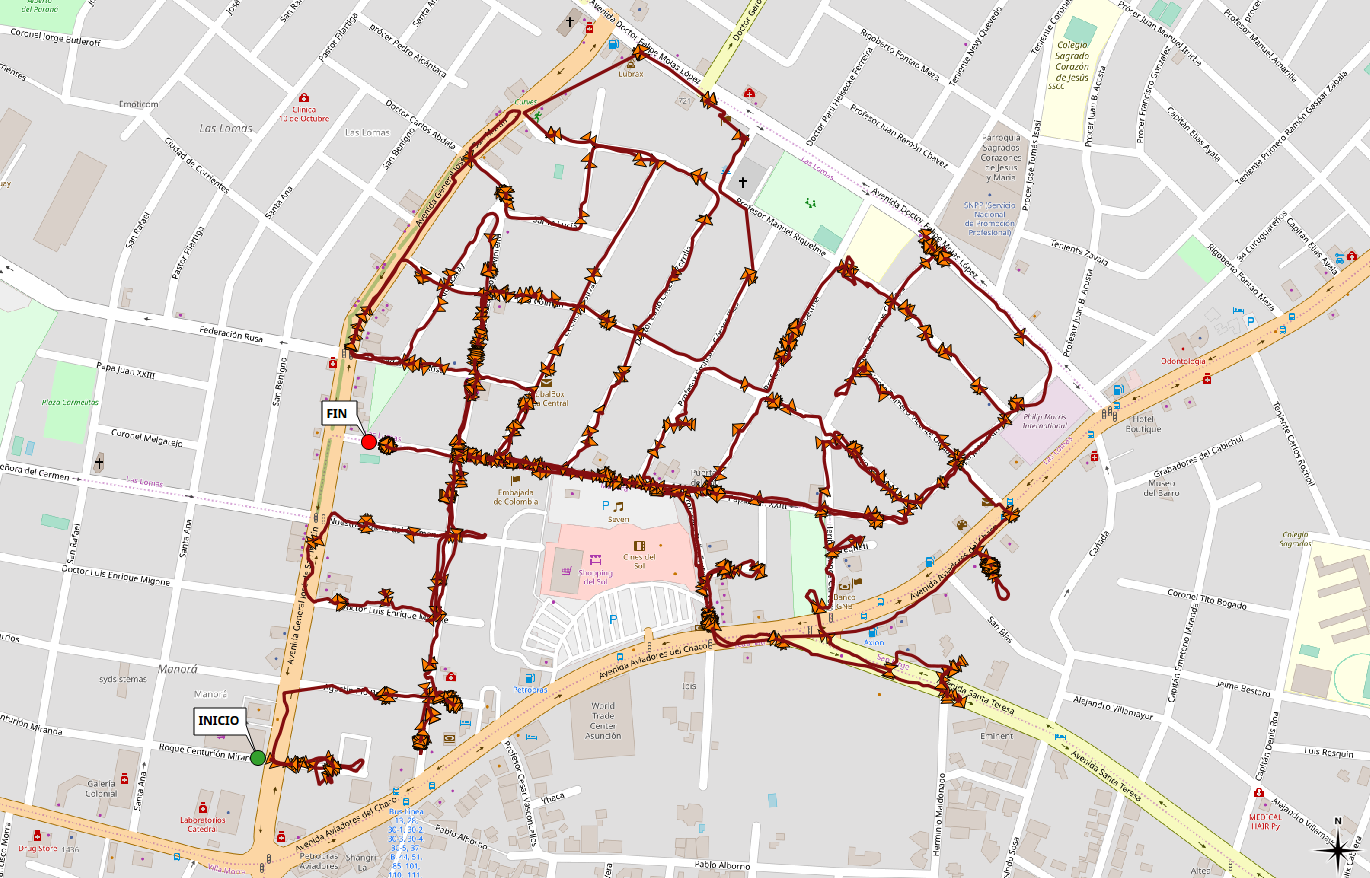
\includegraphics[width=\textwidth]{recorridoActual83.png}
    \caption{Ruta actual. [Fuente: Datos obtenidos en fecha 28/11/2018 del GPS instalado en camión recolector 129 de la DSU]}
    \label{fig:RecorridoActualZona83}
\end{figure}

En la Figura \ref{fig:RecorridoTapeYtyZona83} se muestra el camino generado por \textit{TapeYty} con una cobertura total de las calles que deben ser visitadas en la zona. La secuencia del recorrido se encuentra especificada en los segmentos. La metodología de trabajo se mantiene de acuerdo con lo establecido por la DSU como en la Figura \ref{fig:RecorridoActualZona83}, y por lo tanto, la misma delimitación de zonas.

\begin{figure}[htbp]
    \centering
    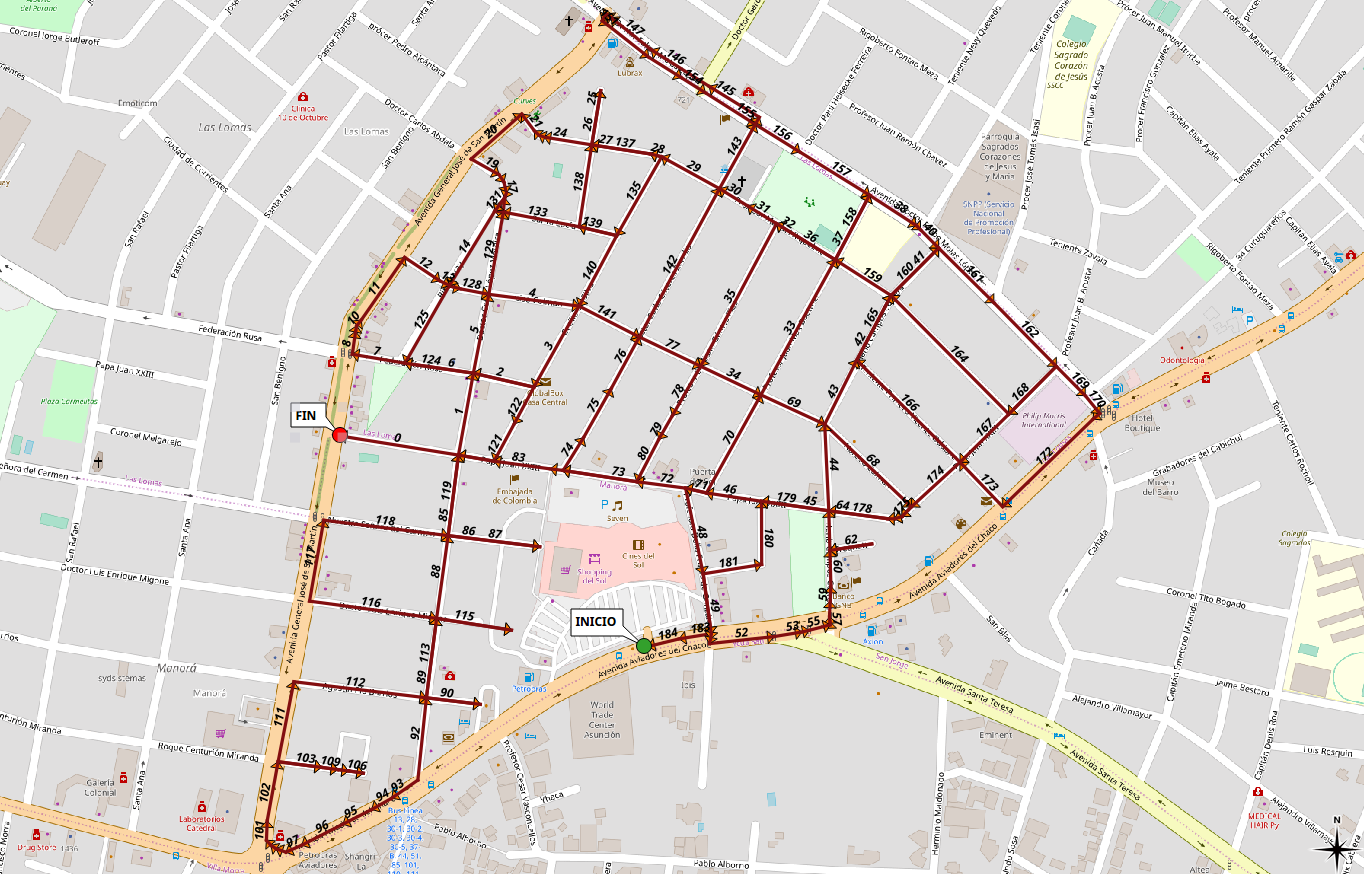
\includegraphics[width=\textwidth]{recorrido83CoberturaTotal.png}
    \caption{Ruta generada por \textit{TapeYty} con cobertura completa.}
    \label{fig:RecorridoTapeYtyZona83}
\end{figure}

Las calles sin salida, las estrechas y las que limitan una zona pero que no deben ser visitadas necesariamente son gestionadas mediante \textit{TapeYty}. Por ejemplo, en la Figura \ref{fig:RecorridoTapeYtyZona83Opcionales} ciertos segmentos de calles pasan a ser opcionales para el paso de camiones simulando el procedimiento llevado a cabo por el equipo de recolección (ver Figura \ref{fig:RecorridoActualZona83}).

% PAPER
% El punto de inicio de la ruta generada se representa en el mapa con un punto verde, el punto final con un punto rojo y la secuencia a seguir se encuentra especificada en los segmentos de calle. Algunos números de secuencia no son visibles en el mapa debido a que los segmentos son muy pequeños y se requiere de acercamiento para verlos, por ejemplo, el sexto segmento a atravesar no es visible debido a su longitud. El sistema permite exportar un archivo con formato GPX (\textit{GPS eXchange Format}) de la ruta generada que es utilizada para la navegación de la ruta.

Algunas zonas cuentan con varios segmentos de calles de un único sentido, y si solo se utilizan los segmentos dentro de la zona, el resultado podría resultar infactible computacionalmente o más costoso en distancia, motivo por el cual se agrega una banda perimetral, tal como en \citet{Braier2017AnArgentina}, de 220 metros representándose a los segmentos de calle dentro de la banda como arcos auxiliares del modelo. Esta situación donde los camiones salen unas cuadras de su zona para volver a entrar es común en la práctica actual de la recolección de residuos.

\begin{figure}[htbp]
    \centering
    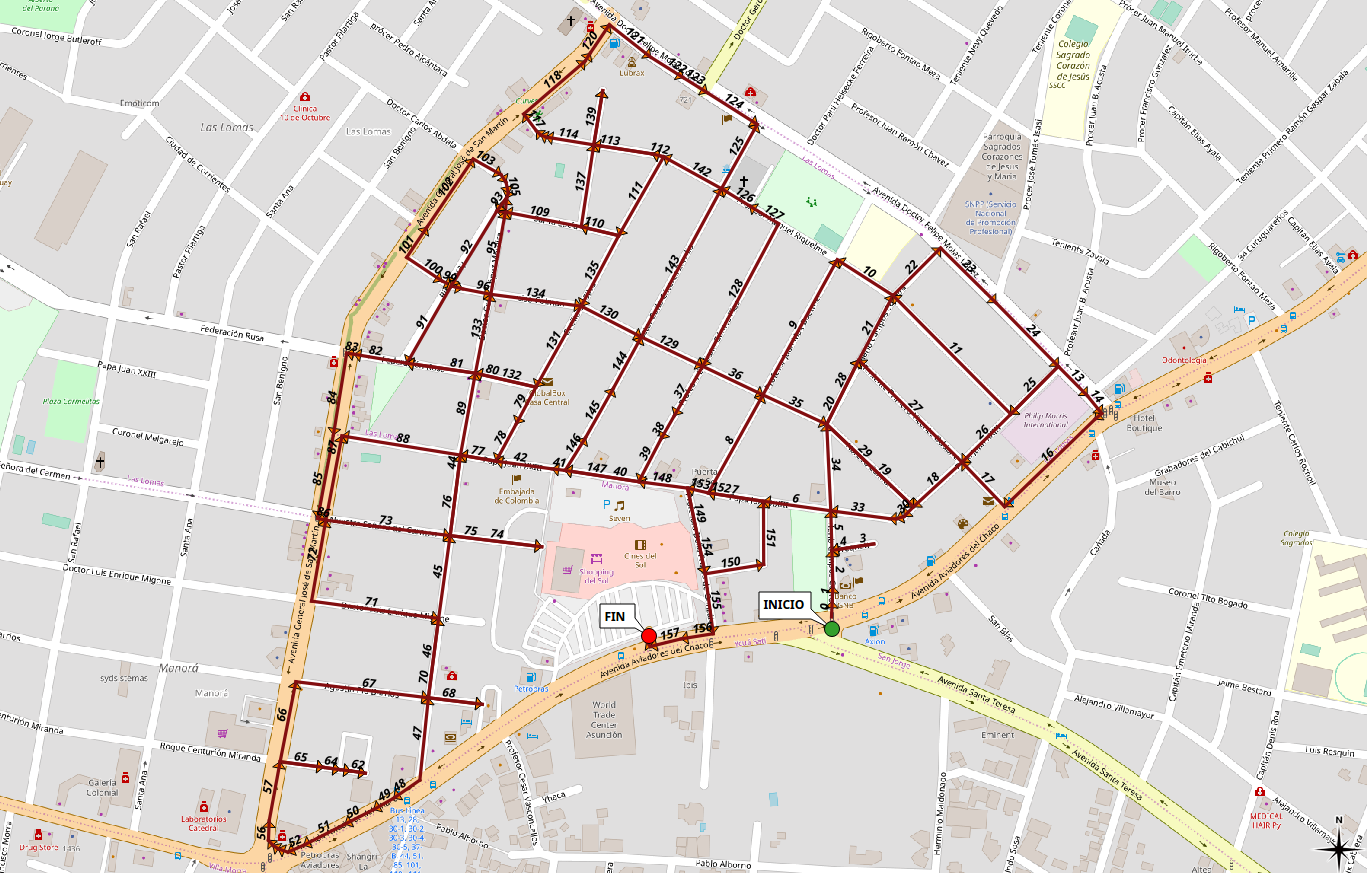
\includegraphics[width=\textwidth]{recorrido83Opcionales.png}
    \caption{Ruta generada por \textit{TapeYty} con segmentos opcionales.}
    \label{fig:RecorridoTapeYtyZona83Opcionales}
\end{figure}

En la Tabla \ref{table:comparacionZona83} se presenta el resultado de la zona 83. En la primera columna se listan las características del modelo: número de iteraciones, los tiempos de ejecución y distancia de la solución. La segunda columna se refiere al escenario en el que todos los segmentos de calles dentro de la zona deben ser visitados por el vehículo recolector y la tercera columna se refiere al escenario en el que 6 segmentos de calles de sentido único y 3 de doble sentido fueron marcados como opcionales desde la aplicación. Si analizamos y comparamos la segunda y tercera columna podemos observar que ambos escenarios coinciden en la cantidad de vértices en el grafo, cantidad de calles de sentido único y de doble sentido, no así en la cantidad de arcos auxiliares debido a la diferencia en la cantidad de segmentos opcionales.

En el primer escenario es posible resolver mediante la técnica de mezcla de subtours recién en la segunda iteración, mientras que en el segundo se puede resolver con la misma técnica ya en la primera iteración. Se observa también que el tiempo de ejecución del modelo es levemente menor para el segundo escenario. Realizar la expansión del grafo a partir de los datos de entrada es el paso que requiere de mayor tiempo en la aplicación. En ambos escenarios se redujo la distancia con respecto al recorrido actual, en el primero en un 20.31\%  y en el segundo un 28.50\%, con 3.44105 km. y 4.82806 km. menos respectivamente.

\begin{table}[htbp]
\caption{Resultados y análisis para la zona 83.}
\begin{tabular}{lll}
\hline
\multirow{2}{*}{Zona 83}                            & \multicolumn{2}{l}{Cobertura de segmentos de calles} \\ \cline{2-3} 
                                                    & Sin opcionales           & Con opcionales           \\ \hline
$|V|$                                                   & 1352                     & 1352                     \\
$|E|$                                                   & 420                      & 420                      \\
$|AM|$                                                  & 256                      & 256                      \\
$|Aaux|$                                                & 1567                     & 1579                     \\
Iteraciones                                         & 2                        & 1                        \\
Tiempo de expansión (s)                      & 20.54530                 & 22.06926                 \\ 
Tiempo de ejecución del modelo (s)            & 0.52790                  & 0.31660                  \\ 
Tiempo de secuenciación (s)                  & 0.04023                  & 0.03425                  \\ 
Distancia (km)                                      & 13.49895                 & 12.11194                 \\ 
Mejora con respecto al actual (\%) & 20.31                    & 28.50                    \\ \hline
\end{tabular}
\label{table:comparacionZona83}
\end{table}

En la Tabla \ref{table:resultadosZonas} se despliegan resultados de tiempos de ejecución de algoritmos y procesos de la optimización de algunas zonas de recolección seleccionadas aleatoriamente. Los resultados de las distintas zonas muestran comportamientos muy similares con respecto a los tiempos. La expansión de zonas siempre requiere de un mayor costo de procesamiento con respecto a los demás tiempos, con registros por encima de 14 segundos y como máximo de 22.5373 segundos. Los tiempos de ejecución del algoritmo de optimización tienen como mayor valor 3.6620 segundos. Por último, los tiempos de secuenciación presentan siempre buen promedio con tiempos entre los rangos 0.0239 y 0.0523 segundos.

% SIMILAR A BRAIER EN ESPANHOL
Si bien la selección para el análisis de resultados fue aleatorio, todas las zonas presentan características similares en tamaño, calles y número de segmentos. Por otra parte, los tiempos de resolución no superaron los 2 minutos para ninguna de las zonas seleccionadas. Estos tiempos son razonables para los requerimientos del sistema. Es importante notar que las rutas obtenidas por este procedimiento fueron bien recibidas por la DSU.

Las rutas actuales informadas en la Tabla \ref{table:comparacionActual} corresponden a datos obtenidos de GPS instalados en los vehículos recolectores por medio de una empresa tercerizada. Estos aparatos están configurados para enviar su ubicación con una frecuencia de 30 segundos generando un margen de error alto con respecto al trazo de las calles de OSM, lo cual influye en la exactitud de las comparaciones. Este problema no se presenció con el recorrido de la zona 83 ya que para ello fue utilizado un GPS configurado por los autores de este trabajo con una frecuencia de 5 segundos.

% DEFINICION DE CAMPUZANO - FPUNA
Para resolver el problema del margen de error se utilizó la estrategia conocida como \textit{Map Matching} (MM). MM es el proceso de identificar la trayectoria seguida por un vehículo en una red de calles a partir de muestras recolectadas acerca de su ubicación. En la Figura \ref{fig:mapMatching} las líneas de color negro representan los datos GPS y las líneas de color verde consiste en la aplicación de la técnica MM con resultados de segmentos coincidentes con el mapa de OSM de la imagen.

La Tabla \ref{table:comparacionActual} presenta la comparación de las distancias de las rutas actuales trazadas con las generadas por \textit{TapeYty}. Como parte del análisis, cabe destacar que los resultados dan un promedio de 19.28\% de mejora con relación al recorrido actual de los camiones considerando los recorridos con calles opcionales. Es interesante destacar que el menor porcentaje de mejora en las rutas con opcionales supera el 10\%.

El ahorro en costos que se puede dar de forma anual es significativo ya que la DSU cuenta con 134 zonas definidas, de las cuales 10 son recorridas 5 días a la semana y el resto 3 veces por semana, durante todo el año. 
%El ahorro en costos que se puede dar de forma anual es significativo.
% El GPS utilizado por los autores de este trabajo en el recorrido de la zona 83 fue configurado con una frecuencia de 5 segundos, motivo por el cual el trazado del camino no cuenta con demasiado margen con respecto al segmento. 

% Los camiones recolectores de la DSU cuentan con dispositivos GPS instalados, reportando la ubicación en tiempo real cada 30 segundos. Para poder identificar la trayectoria seguida es necesario 

\begin{table}[htbp]
\caption{Resultados de ejecución de optimización de zonas.}
\label{table:resultadosZonas}
\resizebox{\textwidth}{!}{%
\begin{tabular}{ccccccccc}
\hline
Nombre de zona     & $|V|$                   & $|E|$                  & $|AM|$                 & $|Aaux|$ & Iteraciones & \begin{tabular}[c]{@{}c@{}}Tiempo de \\ expansión (s)\end{tabular} & \begin{tabular}[c]{@{}c@{}}Tiempo de ejecución \\ del modelo (s)\end{tabular} & \begin{tabular}[c]{@{}c@{}}Tiempo de \\ secuenciación (s)\end{tabular} \\ \hline
71                 & \multirow{2}{*}{1098} & \multirow{2}{*}{404} & \multirow{2}{*}{145} & 1396   & 1           & 18.8936                                                            & 0.2044                                                                        & 0.0330                                                                 \\
71 con opcionales  &                       &                      &                      & 1407   & 1           & 17.9064                                                            & 0.2143                                                                        & 0.0311                                                                 \\ \hline
3                  & \multirow{2}{*}{886}  & \multirow{2}{*}{234} & \multirow{2}{*}{209} & 1105   & 2           & 15.5142                                                            & 0.4226                                                                        & 0.0461                                                                 \\
3 con opcionales   &                       &                      &                      & 1116   & 1           & 14.7611                                                            & 0.2189                                                                        & 0.0417                                                                 \\ \hline
119                & \multirow{2}{*}{1458} & \multirow{2}{*}{654} & \multirow{2}{*}{75}  & 1716   & 3           & 22.5373                                                            & 2.2673                                                                        & 0.0523                                                                 \\
119 con opcionales &                       &                      &                      & 1746   & 1           & 22.5269                                                            & 3.6620                                                                        & 0.0388                                                                 \\ \hline
21                 & \multirow{2}{*}{932}  & \multirow{2}{*}{290} & \multirow{2}{*}{176} & 1067   & 2           & 14.8009                                                            & 0.3358                                                                        & 0.0326                                                                 \\
21 con opcionales  &                       &                      &                      & 1076   & 2           & 14.5501                                                            & 0.3946                                                                        & 0.0239                                                                 \\ \hline
22                 & \multirow{2}{*}{1056} & \multirow{2}{*}{358} & \multirow{2}{*}{170} & 1280   & 3           & 17.1519                                                            & 2.0509                                                                        & 0.0348                                                                 \\
22 con opcionales  &                       &                      &                      & 1308   & 5           & 16.8168                                                            & 1.8977                                                                        & 0.0290                                                                 \\ \hline
83                 & \multirow{2}{*}{1352} & \multirow{2}{*}{420} & \multirow{2}{*}{256} & 1567   & 2           & 20.5453                                                            & 0.5279                                                                        & 0.0402                                                                 \\
83 con opcionales  &                       &                      &                      & 1579   & 1           & 22.0693                                                            & 0.3166                                                                        & 0.0342                                                                 \\ \hline
\end{tabular}%
}
\end{table}

\begin{figure}[htbp]
    \centering
    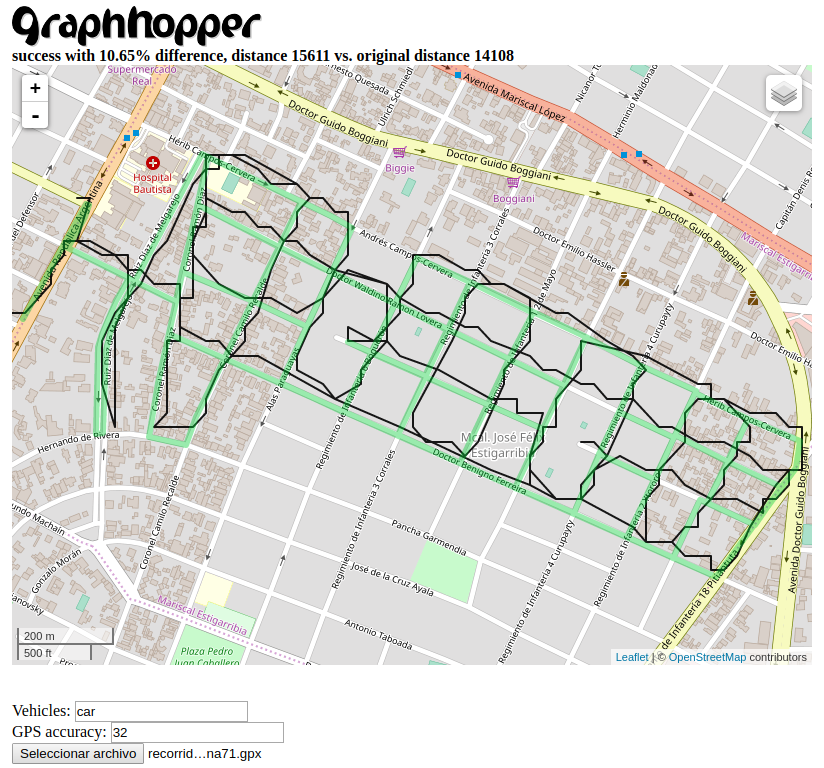
\includegraphics[width=\textwidth]{graphhopper71.png}
    \caption{Técnica \textit{Map Matching} aplicada sobre datos GPS de la DSU utilizando la herramienta \textit{Open Source} Graphhopper.}
    \label{fig:mapMatching}
\end{figure}

\begin{table}[tbp]
\caption{Comparación de resultados obtenidos con el actual.}
\label{table:comparacionActual}
\resizebox{\textwidth}{!}{%
\begin{tabular}{cccc}
\hline
Nombre de zona     & \begin{tabular}[c]{@{}c@{}}Distancia actual (km) \\ con Map matching\end{tabular} & Distancia generada (km) & \begin{tabular}[c]{@{}c@{}}Mejora con respecto \\ al actual (\%)\end{tabular} \\ \hline
71                 & \multirow{2}{*}{15.611}                                                           & 14.358                  & 8.02                                                                          \\
71 con opcionales  &                                                                                   & 13.320                  & 14.67                                                                         \\ \hline
3                  & \multirow{2}{*}{19.486}                                                           & 17.851                  & 8.39                                                                          \\
3 con opcionales   &                                                                                   & 16.879                  & 13.38                                                                         \\ \hline
119                & \multirow{2}{*}{16.940}                                                           & 14.704                  & 13.19                                                                         \\
119 con opcionales &                                                                                   & 13.825                  & 18.38                                                                         \\ \hline
21                 & \multirow{2}{*}{14.895}                                                           & 13.003                  & 12.7                                                                          \\
21 con opcionales  &                                                                                   & 11.675                  & 21.62                                                                         \\ \hline
22                 & \multirow{2}{*}{14.382}                                                           & 12.622                  & 12.24                                                                         \\
22 con opcionales  &                                                                                   & 11.635                  & 19.1                                                                          \\ \hline
83                 & \multirow{2}{*}{16.940}                                                           & 13.499                  & 20.31                                                                         \\
83 con opcionales  &                                                                                   & 12.112                  & 28.5                                                                          \\ \hline
\end{tabular}%
}
\end{table}

\section{Calidad de Software}

Existen varias definiciones para el concepto de Calidad de Software y la mayoría suele coincidir en la idea de adecuación a los requerimientos. La calidad de software está definida en \citet{Pressman2010IngenieriaPractico} como ``el proceso eficaz de software que se aplica de manera que crea un producto útil que proporciona valor medible a quienes lo producen y a quienes lo utilizan''. La ISO/IEC 9126 la define como ``el grado con el que un sistema, componente o proceso cumple los requerimientos especificados y las necesidades o expectativas del cliente o usuario''. 

Entre los atributos de la Calidad del Software tenemos: seguridad, fiabilidad, flexibilidad, robustez, comprensibilidad, testeabilidad, adaptabilidad, modularidad, complejidad, portababilidad, usabilidad, reusabilidad, eficiencia y facilidad.

A continuación se muestra un reporte con las métricas de algunos atributos de calidad en los proyectos \textit{backend} y \textit{frontend} de la aplicación. Las incidencias encontradas en ambos proyectos se fueron solucionando y corrigiendo. Se utilizaron las reglas por defecto proporcionadas por la herramienta utilizada SonarQube. (Ver Figuras \ref{fig:QAbackend}, \ref{fig:QAfrontend})

SonarQube define tres tipos de problemas:

\begin{itemize}
    \item \textit{Bug}: Un error de codificación que romperá su código y debe solucionarse de inmediato.
    \item \textit{Vulnerability}: Un punto en su código que está abierto al ataque.
    \item \textit{Code smell}: Un problema de mantenibilidad que hace que su código sea confuso y difícil de mantener.
\end{itemize}

Cada problema corresponde a una de las cinco severidades:

\begin{itemize}
    \item \textit{Blocker}: Error con una alta probabilidad de afectar el comportamiento de la aplicación en producción: pérdida de memoria, conexión JDBC no cerrada, etc. El código debe ser arreglado de inmediato.
    \item \textit{Critical}: Ya sea un error con poca probabilidad de afectar el comportamiento de la aplicación en producción o un problema que representa un defecto de seguridad: bloque de captura vacío, inyección de SQL, etc. El código debe revisarse de inmediato.
    \item \textit{Major}: Defecto de calidad que puede tener un gran impacto en la productividad del desarrollador: pieza de código descubierta, bloques duplicados, parámetros no utilizados.
    \item \textit{Minor}: Defecto de calidad que puede afectar ligeramente la productividad del desarrollador: las líneas no deben ser demasiado largas, las declaraciones de "cambio" deben tener al menos 3 casos, entre otros.
    \item \textit{Info}: Ni un error ni un defecto de calidad, solo un hallazgo.
\end{itemize}

\begin{figure}[htbp]
    \centering
    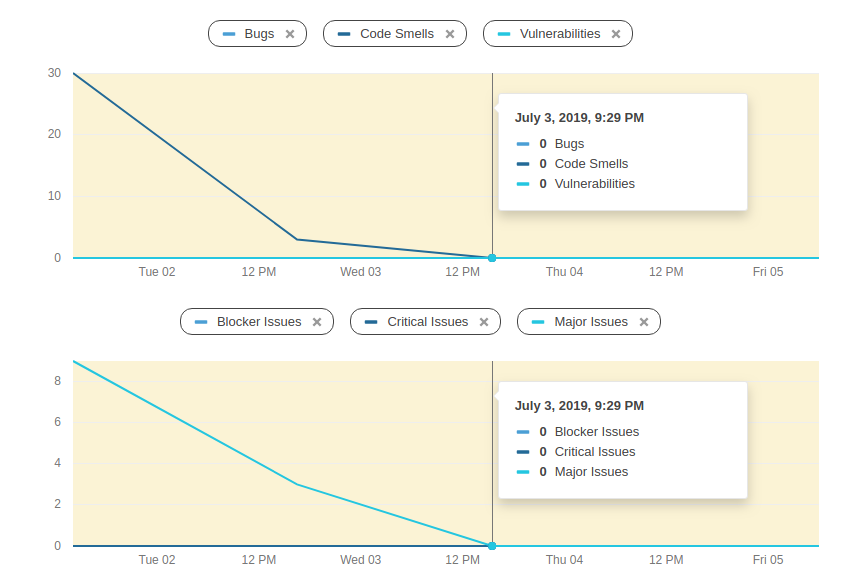
\includegraphics[width=\textwidth]{reporteQA_BE.png}
    \caption{Reporte de inspección de código con SonarQube del \textit{Backend}.}
    \label{fig:QAbackend}
\end{figure}

\begin{figure}[htbp]
    \centering
    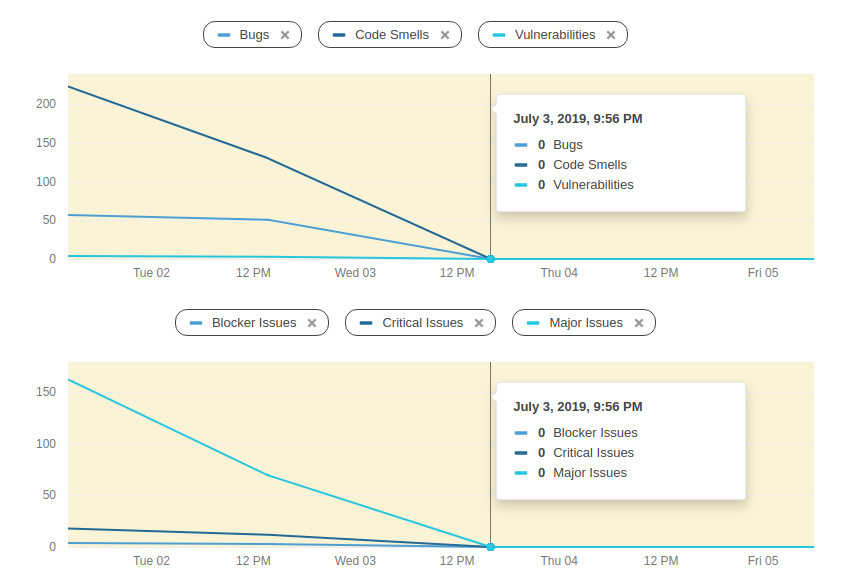
\includegraphics[width=\textwidth]{reporteQA_FE2.png}
    \caption{Reporte de inspección de código con SonarQube del \textit{Frontend}.}
    \label{fig:QAfrontend}
\end{figure}

% \subsection{Usabilidad} % Resultados y Discusión

\clearpage
\lhead{\emph{Conclusión}} 
\renewcommand\chaptername{Capítulo}%título "Capítulo"
\def\baselinestretch{1}
\chapter{Conclusiones y Trabajos Futuros}

\markboth{\hfill \thechapter. Conclusiones y Trabajos Futuros}{\hfill \thechapter. Conclusiones y Trabajos Futuros}

\section {Conclusiones del trabajo}

 % Conclusión

%% --------------- Apéndices --------------------------------------

\clearpage
\appendix
\lhead{\emph{Apéndice A}} 
\renewcommand{\appendixname}{Apéndice}
\chapter\bigskip
\ifpdf
  \graphicspath{{AppendixA/AppendixAFigs/PNG/}{AppendixA/AppendixAFigs/PDF/}{AppendixA/AppendixAFigs/}}
\else
  \graphicspath{{AppendixA/AppendixAFigs/EPS/}{AppendixA/AppendixAFigs/}}
\fi

\section{Valores de las métricas seleccionadas en las imágenes de referencias.}
\begin{figure}[H]
    \begin{center}
        \subfigure[][\label{fig:img1} $SSIM = 1$ \newline $LTG = 1 $ \newline $\mathscr{H} = 7.4428$ \newline $\mathscr E =3.4754$]
        {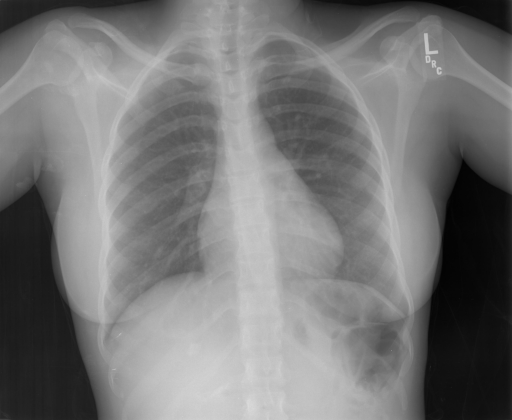
\includegraphics[width=4.5cm]{AppendixA/AppendixAFigs/originales/frontales/imagen1.png}}
        \subfigure[][\label{fig:img2} $SSIM = 1$ \newline $LTG = 1$ \newline $\mathscr{H} = 6.6690$ \newline $\mathscr E =2.9755$
        ]{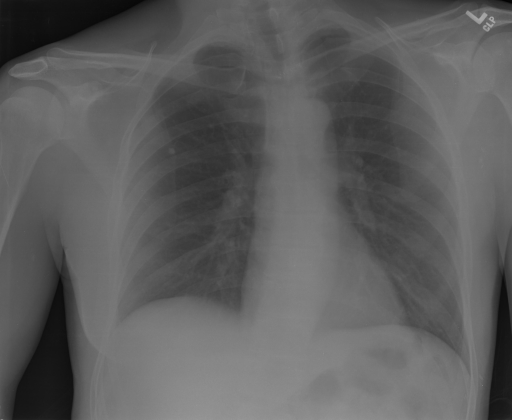
\includegraphics[width=4.5cm]{AppendixA/AppendixAFigs/originales/frontales/imagen2.png}}
        \subfigure[][\label{fig:img4} $SSIM = 1$ \newline $LTG = 1$ \newline $\mathscr{H} = 7.1196$ \newline $\mathscr E =3.4570$
        ]{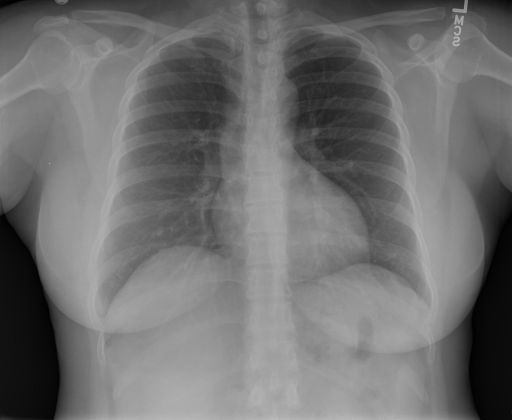
\includegraphics[width=4.5cm]{AppendixA/AppendixAFigs/originales/frontales/imagen4.png}}
    \end{center}
    \label{fig:gral1}
\end{figure}

\begin{figure}[H]
    \begin{center}
        \subfigure[][\label{fig:img3} $SSIM = 1$ \newline $LTG = 1$ \newline $\mathscr{H} = 7.3003$ \newline $\mathscr E =3.7876$
        ]{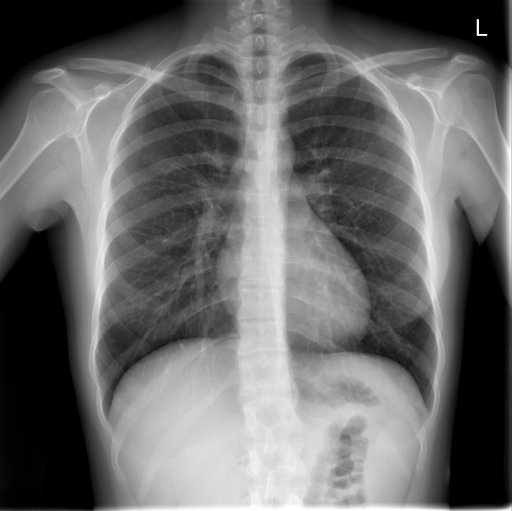
\includegraphics[width=4.5cm]{AppendixA/AppendixAFigs/originales/frontales/imagen3.png}}
        \subfigure[][\label{fig:img5} $SSIM = 1$ \newline $LTG = 1$ \newline $\mathscr{H} = 7.4409$ \newline $\mathscr E =3.5873$
        ]{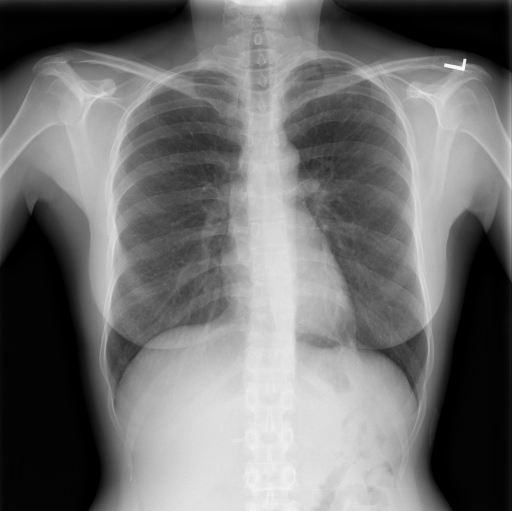
\includegraphics[width=4.5cm]{AppendixA/AppendixAFigs/originales/frontales/imagen5.png}}
        \subfigure[][\label{fig:img7} $SSIM = 1$ \newline $LTG = 1$ \newline $\mathscr{H} = 7.7184$ \newline $\mathscr E =3.9015$
        ]{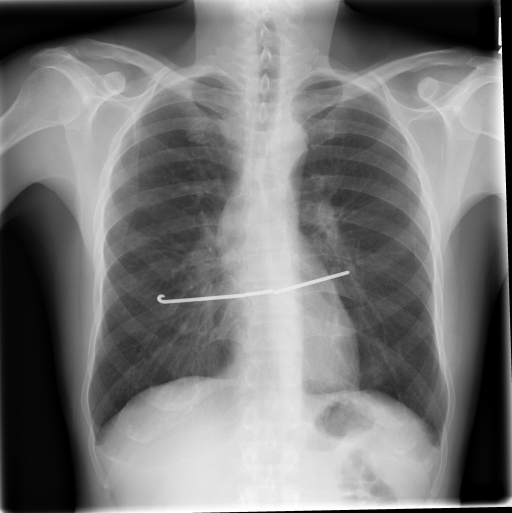
\includegraphics[width=4.5cm]{AppendixA/AppendixAFigs/originales/frontales/imagen7.png}}
    \end{center}
    \label{fig:gral2}
\end{figure}

\begin{figure}[H]
    \begin{center}
        \subfigure[][\label{fig:img6}  $SSIM = 1$ \newline $LTG = 1$ \newline $\mathscr{H} = 6.8287$ \newline $\mathscr E =3.1996$
        ]{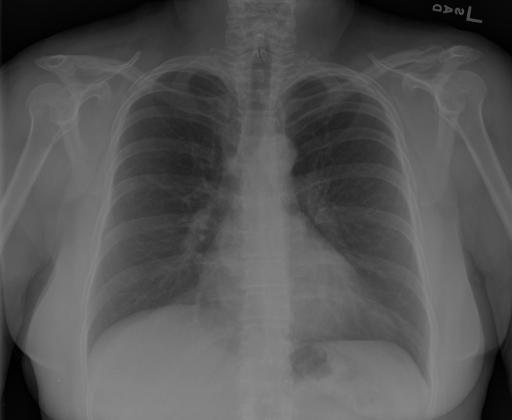
\includegraphics[width=4.5cm]{AppendixA/AppendixAFigs/originales/frontales/imagen6.png}}
        \subfigure[][\label{fig:img8}  $SSIM = 1$ \newline $LTG = 1$ \newline $\mathscr{H} = 6.8998$ \newline $\mathscr E =3.3196$
        ]{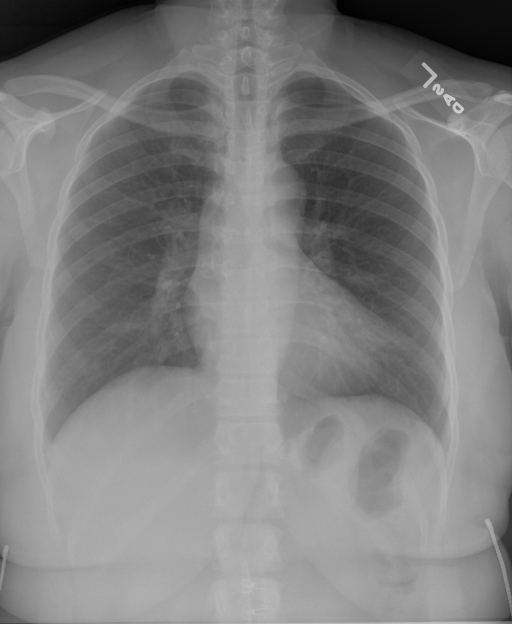
\includegraphics[width=3.0cm]{AppendixA/AppendixAFigs/originales/frontales/imagen8.png}}
        \subfigure[][\label{fig:img9}  $SSIM = 1$ \newline $LTG =1 $ \newline $\mathscr{H} = 6.6672$ \newline $\mathscr E =3.4084$
        ]{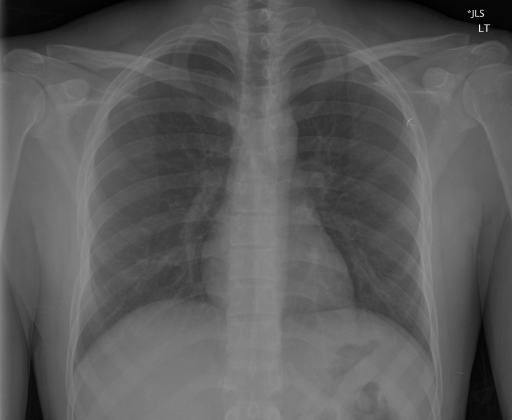
\includegraphics[width=4.5cm]{AppendixA/AppendixAFigs/originales/frontales/imagen9.png}}
    \end{center}
    \label{fig:gral3}
\end{figure}

\begin{figure}[H]
    \begin{center}
        \subfigure[][\label{fig:img10}  $SSIM = 1$ \newline $LTG = 1$ \newline $\mathscr{H} = 6.8803$ \newline $\mathscr E =3.3658$
        ]{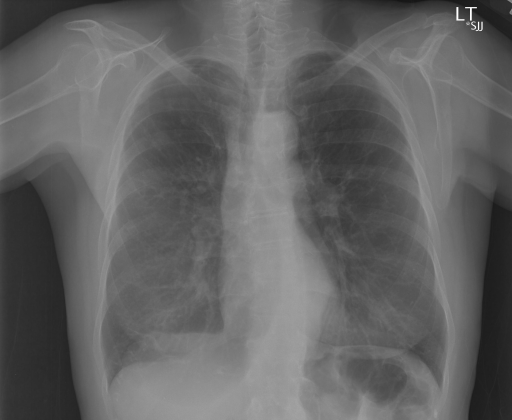
\includegraphics[width=4.5cm]{AppendixA/AppendixAFigs/originales/frontales/imagen10.png}}
        \subfigure[][\label{fig:img11}  $SSIM = 1$ \newline $LTG = 1$ \newline $\mathscr{H} = 7.5582$ \newline $\mathscr E =3.5560$
        ]{\includegraphics[width=3.7cm]{AppendixA/AppendixAFigs/originales/frontales/imagen11.png}}
        \subfigure[][\label{fig:img12}  $SSIM = 1$ \newline $LTG = 1$ \newline $\mathscr{H} = 6.5775$ \newline $\mathscr E =3.02324.1202$
        ]{\includegraphics[width=4.5cm]{AppendixA/AppendixAFigs/originales/frontales/imagen12.png}}
    \end{center}
    \label{fig:gral4}
\end{figure}

\begin{figure}[H]
    \begin{center}
        \subfigure[][\label{fig:img13}  $SSIM = 1$ \newline $LTG = 1$ \newline $\mathscr{H} = 7.5991$ \newline $\mathscr E =4.1202$
        ]{\includegraphics[width=4.5cm]{AppendixA/AppendixAFigs/originales/frontales/imagen13.png}}
        \subfigure[][\label{fig:img14}  $SSIM = 1$ \newline $LTG = 1$ \newline $\mathscr{H} = 6.9048$ \newline $\mathscr E =3.4270$
        ]{\includegraphics[width=4.5cm]{AppendixA/AppendixAFigs/originales/frontales/imagen14.png}}
        \subfigure[][\label{fig:img15}  $SSIM = 1$ \newline $LTG = 1$ \newline $\mathscr{H} = 6.7262$ \newline $\mathscr E =3.1108$
        ]{\includegraphics[width=4.5cm]{AppendixA/AppendixAFigs/originales/frontales/imagen15.png}}
    \end{center}
    \label{fig:gral5}
\end{figure}


\begin{figure}[H]
    \begin{center}
        \subfigure[][\label{fig:imgtll} $SSIM = 1$ \newline $LTG = 1 $ \newline $\mathscr{H} = 7.2447$ \newline $\mathscr E = 2.8626$]
        {\includegraphics[width=4cm]{AppendixA/AppendixAFigs/originales/laterales/imagen1.png}}
        \subfigure[][\label{fig:imgtl2} $SSIM = 1$ \newline $LTG = 1$ \newline $\mathscr{H} =7.1010 $ \newline $\mathscr E = 2.8157$
        ]{\includegraphics[width=4cm]{AppendixA/AppendixAFigs/originales/laterales/imagen2.png}}
        \subfigure[][\label{fig:imgtl4} $SSIM = 1$ \newline $LTG = 1 $ \newline $\mathscr{H} = 6.7004$ \newline $\mathscr E = 2.7408$]
        {\includegraphics[width=4cm]{AppendixA/AppendixAFigs/originales/laterales/imagen4.png}}
    \end{center}
    \label{fig:gral6}
\end{figure}

\begin{figure}[H]
    \begin{center}
       
        \subfigure[][\label{fig:imgtl6} $SSIM = 1$ \newline $LTG = 1$ \newline $\mathscr{H} = 5.8141$ \newline $\mathscr E = 1.9030$
        ]{\includegraphics[width=4cm]{AppendixA/AppendixAFigs/originales/laterales/imagen6.png}}
       \subfigure[][\label{fig:imgtl7} $SSIM = 1$ \newline $LTG = 1 $ \newline $\mathscr{H} = 6.9070$ \newline $\mathscr E = 2.9594$]
        {\includegraphics[width=4cm]{AppendixA/AppendixAFigs/originales/laterales/imagen7.png}}
        \subfigure[][\label{fig:imgtl8} $SSIM = 1$ \newline $LTG = 1$ \newline $\mathscr{H} = 7.0622$ \newline $\mathscr E = 2.9446$
        ]{\includegraphics[width=4cm]{AppendixA/AppendixAFigs/originales/laterales/imagen8.png}}
    \end{center}
    \label{fig:gral7}
\end{figure}

\begin{figure}[H]
    \begin{center}
        
        \subfigure[][\label{fig:imgtl9} $SSIM = 1$ \newline $LTG = 1$ \newline $\mathscr{H} = 7.5625$ \newline $\mathscr E = 3.4395$
        ]{\includegraphics[width=4cm]{AppendixA/AppendixAFigs/originales/laterales/imagen9.png}}
        \subfigure[][\label{fig:imgtl10} $SSIM = 1$ \newline $LTG = 1 $ \newline $\mathscr{H} = 7.1064$ \newline $\mathscr E = 3.3058$]
        {\includegraphics[width=4cm]{AppendixA/AppendixAFigs/originales/laterales/imagen10.png}}
        \subfigure[][\label{fig:imgtl11} $SSIM = 1$ \newline $LTG = 1$ \newline $\mathscr{H} = 6.2748$ \newline $\mathscr E = 2.4087$
        ]{\includegraphics[width=4cm]{AppendixA/AppendixAFigs/originales/laterales/imagen11.png}}
    \end{center}
    \label{fig:gral8}
\end{figure}

\begin{figure}[H]
    \begin{center}
        \subfigure[][\label{fig:imgtl3} $SSIM = 1$ \newline $LTG = 1$ \newline $\mathscr{H} = 5.7765$ \newline $\mathscr E = 2.4201$
        ]{\includegraphics[width=4.5cm]{AppendixA/AppendixAFigs/originales/laterales/imagen3.png}}
        \subfigure[][\label{fig:imgtl5} $SSIM = 1$ \newline $LTG = 1$ \newline $\mathscr{H} = 6.4335$ \newline $\mathscr E =2.7586$
        ]{\includegraphics[width=4.5cm]{AppendixA/AppendixAFigs/originales/laterales/imagen5.png}}
    \end{center}
    \label{fig:gral9}
\end{figure}


\section{Resultado Correlación de Pearson}

\begin{table}[H]
\centering
\caption{Promedio de la correlación de Pearson.}
\begin{tabular}{|c|c|}
\hline
Métricas & Correlación \\
\hline \hline 
%-0.9547657122	-0.9866466591	-0.9308066035	-0.9731620476
$\mathscr{H}$ / \textit{SSIM} & -0.9554 \\ \hline
$\mathscr{E}$ / \textit{SSIM} & \textbf{-0.9870}\\ \hline
$\mathscr{H}$ / \textit{LTG} & -0.9319 \\ \hline
$\mathscr{E}$ / \textit{LTG} & -0.9731 \\ \hline
\end{tabular}
\label{tabla:promcorrelacion}
\centering
\end{table}

\section{Resultados Indicador de Hipervolumen}

\begin{table}[H]
\centering
\caption{Hipervolumen de los Frentes Pareto - Tórax Frontal.}
\begin{tabular}{|c|c|}
\hline
Frente Pareto & Valor Hipervolumen {\it yref}: [6,1] \\
\hline \hline 
\it{Robusto} &  0.9987\\ \hline
\it{Tórax Frontal \ref{fig:img1}} & 0.97088 \\ \hline
\it{Tórax Frontal \ref{fig:img2}} & 1.07444 \\ \hline
\it{Tórax Frontal \ref{fig:img4}} & 0.94675 \\ \hline
\it{Tórax Frontal \ref{fig:img3}} & 0.98474 \\ \hline
\it{Tórax Frontal \ref{fig:img5}} & 1.18447 \\ \hline
\it{Tórax Frontal \ref{fig:img7}} & 0.89804 \\ \hline
\it{Tórax Frontal \ref{fig:img6}} & 1.05435 \\ \hline
\it{Tórax Frontal \ref{fig:img8}} & 0.94021 \\ \hline
\it{Tórax Frontal \ref{fig:img9}} & 0.79659 \\ \hline
\it{Tórax Frontal \ref{fig:img10}} & 0.89486 \\ \hline
\it{Tórax Frontal \ref{fig:img11}} & 0.97175 \\ \hline
\it{Tórax Frontal \ref{fig:img12}} & 1.08461 \\ \hline
\it{Tórax Frontal \ref{fig:img13}} & 0.62923 \\ \hline
\it{Tórax Frontal \ref{fig:img14}} & 0.85066 \\ \hline
\it{Tórax Frontal \ref{fig:img15}} & 0.90512 \\ \hline
\end{tabular}
\label{tabla:hipervolumen-frontal}
\end{table}

\begin{table}[H]
\centering
\caption{Hipervolumen de los Frentes Pareto - Tórax Lateral.}
\begin{tabular}{|c|c|}
\hline
Frente Pareto & Valor  Hipervolumen {\it yref}: [6,1] \\
\hline \hline 
\it{Robusto} &  1.51317\\ \hline
\it{Tórax Lateral \ref{fig:imgtll}} & 1.29874 \\ \hline
\it{Tórax Lateral \ref{fig:imgtl2}} & 1.47126 \\ \hline
\it{Tórax Lateral \ref{fig:imgtl4}} & 1.34961 \\ \hline
\it{Tórax Lateral \ref{fig:imgtl6}} & 1.77041 \\ \hline
\it{Tórax Lateral \ref{fig:imgtl7}} & 1.15427 \\ \hline
\it{Tórax Lateral \ref{fig:imgtl8}} & 1.13405 \\ \hline
\it{Tórax Lateral \ref{fig:imgtl9}} & 1.02208 \\ \hline
\it{Tórax Lateral \ref{fig:imgtl10}} & 1.27029 \\ \hline
\it{Tórax Lateral \ref{fig:imgtl11}} & 1.45903 \\ \hline
\it{Tórax Lateral \ref{fig:imgtl3}} & 2.45754 \\ \hline
\it{Tórax Lateral \ref{fig:imgtl5}} & 1.63800 \\ \hline

\end{tabular}
\label{tabla:hipervolumen-lateral}
\end{table}



% \bigskip












	% Appendix Title


\lhead{\emph{Apéndice B}} 
\renewcommand{\appendixname}{Apéndice}
% \chapter\bigskip
% \ifpdf
%   \graphicspath{{AppendixB/AppendixBFigs/PNG/}{AppendixB/AppendixBFigs/PDF/}{AppendixB/AppendixBFigs/}}
% \else
%   \graphicspath{{AppendixB/AppendixBFigs/EPS/}{AppendixB/AppendixBFigs/}}
% \fi

% \section{Frente Pareto Robusto y óptimo de cada imagen de referencia}

% \begin{figure}[H]
%     \centering
%         \subfigure[][\label{a}Tórax Frontal \ref{fig:img1}]{\includegraphics[width=7cm]{AppendixB/AppendixBFigs/FP-torax_frontal/img1-FP-TF-robusto.png}}
%         \subfigure[][\label{b}Tórax Frontal \ref{fig:img2}]{\includegraphics[width=7cm]{AppendixB/AppendixBFigs/FP-torax_frontal/img2-FP-TF-robusto.png}}
   
%     \caption {Frente Pareto Entropía Local - SSIM. Tórax Frontal\\}{
%     {\color{myblue} {$\bullet$}} Frente pareto robusto \\
%     {\color{mygreen} {$\bullet$}} Frente pareto óptimo}
%     \label{fp-robusto-optimo-tf1}
% \end{figure}



% \begin{figure}[H]
%     \centering
%         \subfigure[][\label{a} Tórax Frontal \ref{fig:img4}]{\includegraphics[width=7cm]{AppendixB/AppendixBFigs/FP-torax_frontal/img4-FP-TF-robusto.png}}
%         \subfigure[][\label{b} Tórax Frontal \ref{fig:img3}]{\includegraphics[width=7cm]{AppendixB/AppendixBFigs/FP-torax_frontal/img3-FP-TF-robusto.png}}
   
%   \caption {Frente Pareto Entropía Local - SSIM. Tórax Frontal\\}{
%     {\color{myblue} {$\bullet$}} Frente pareto robusto \\
%     {\color{mygreen} {$\bullet$}} Frente pareto óptimo}
%     \label{fp-robusto-optimo-tf2}
% \end{figure}


% \begin{figure}[H]
%     \centering
%         \subfigure[][\label{a} Tórax Frontal \ref{fig:img5}]{\includegraphics[width=7cm]{AppendixB/AppendixBFigs/FP-torax_frontal/img5-FP-TF-robusto.png}}
%         \subfigure[][\label{b} Tórax Frontal \ref{fig:img7}]{\includegraphics[width=7cm]{AppendixB/AppendixBFigs/FP-torax_frontal/img7-FP-TF-robusto.png}}
   
%     \caption {Frente Pareto Entropía Local - SSIM. Tórax Frontal\\}{
%     {\color{myblue} {$\bullet$}} Frente pareto robusto \\
%     {\color{mygreen} {$\bullet$}} Frente pareto óptimo}
%     \label{fp-robusto-optimo-tf3}
% \end{figure}

% \begin{figure}[H]
%     \centering
%         \subfigure[][\label{a} Tórax Frontal \ref{fig:img6}]{\includegraphics[width=7cm]{AppendixB/AppendixBFigs/FP-torax_frontal/img6-FP-TF-robusto.png}}
%         \subfigure[][\label{b} Tórax Frontal \ref{fig:img8}]{\includegraphics[width=7cm]{AppendixB/AppendixBFigs/FP-torax_frontal/img8-FP-TF-robusto.png}}
   
%     \caption {Frente Pareto Entropía Local - SSIM. Tórax Frontal\\}{
%     {\color{myblue} {$\bullet$}} Frente pareto robusto \\
%     {\color{mygreen} {$\bullet$}} Frente pareto óptimo}
%     \label{fp-robusto-optimo-tf4}
% \end{figure}

% \begin{figure}[H]
%     \centering
%         \subfigure[][\label{a} Tórax Frontal \ref{fig:img9}]{\includegraphics[width=7cm]{AppendixB/AppendixBFigs/FP-torax_frontal/img9-FP-TF-robusto.png}}
%         \subfigure[][\label{b} Tórax Frontal \ref{fig:img10}]{\includegraphics[width=7cm]{AppendixB/AppendixBFigs/FP-torax_frontal/img10-FP-TF-robusto.png}}
   
%     \caption {Frente Pareto Entropía Local - SSIM. Tórax Frontal\\}{
%     {\color{myblue} {$\bullet$}} Frente pareto robusto \\
%     {\color{mygreen} {$\bullet$}} Frente pareto óptimo}
%     \label{fp-robusto-optimo-tf5}
% \end{figure}

% \begin{figure}[H]
%     \centering
%         \subfigure[][\label{a} Tórax Frontal \ref{fig:img11}]{\includegraphics[width=7cm]{AppendixB/AppendixBFigs/FP-torax_frontal/img11-FP-TF-robusto.png}}
%         \subfigure[][\label{b} Tórax Frontal \ref{fig:img12}]{\includegraphics[width=7cm]{AppendixB/AppendixBFigs/FP-torax_frontal/img12-FP-TF-robusto.png}}
%      \caption {Frente Pareto Entropía Local - SSIM. Tórax Frontal\\}{
%     {\color{myblue} {$\bullet$}} Frente pareto robusto \\
%     {\color{mygreen} {$\bullet$}} Frente pareto óptimo}
%     \label{fp-robusto-optimo-tf6}
% \end{figure}

% \begin{figure}[H]
%     \centering
%         \subfigure[][\label{a} Tórax Frontal \ref{fig:img13}]{\includegraphics[width=7cm]{AppendixB/AppendixBFigs/FP-torax_frontal/img13-FP-TF-robusto.png}}
%         \subfigure[][\label{b} Tórax Frontal \ref{fig:img14}]{\includegraphics[width=7cm]{AppendixB/AppendixBFigs/FP-torax_frontal/img14-FP-TF-robusto.png}}
%      \caption {Frente Pareto Entropía Local - SSIM. Tórax Frontal\\}{
%     {\color{myblue} {$\bullet$}} Frente pareto robusto \\
%     {\color{mygreen} {$\bullet$}} Frente pareto óptimo}
%     \label{fp-robusto-optimo-tf7}
% \end{figure}

% \begin{figure}[H]
%     \centering
%         \subfigure[][\label{a} Tórax Frontal \ref{fig:img15}]{\includegraphics[width=7cm]{AppendixB/AppendixBFigs/FP-torax_frontal/img15-FP-TF-robusto.png}}
%      \caption {Frente Pareto Entropía Local - SSIM. Tórax Frontal\\}{
%     {\color{myblue} {$\bullet$}} Frente pareto robusto \\
%     {\color{mygreen} {$\bullet$}} Frente pareto óptimo}
%     \label{fp-robusto-optimo-tf8}
% \end{figure}


% \begin{figure}[H]
%     \centering
%         \subfigure[][\label{a} Tórax Lateral \ref{fig:imgtll}]{\includegraphics[width=7cm]{AppendixB/AppendixBFigs/FP-torax_lateral/img1-FP-TL-robusto.png}}
%         \subfigure[][\label{a} Tórax Lateral \ref{fig:imgtl2}]{\includegraphics[width=7cm]{AppendixB/AppendixBFigs/FP-torax_lateral/img4-FP-TL-robusto.png}}
%      \caption {Frente Pareto Entropía Local - SSIM. Tórax Lateral\\}{
%     {\color{myblue} {$\bullet$}} Frente pareto robusto \\
%     {\color{mygreen} {$\bullet$}} Frente pareto óptimo}
%     \label{fp-robusto-optimo-tl1}
% \end{figure}

% \begin{figure}[H]
%     \centering
%         \subfigure[][\label{a} Tórax Lateral \ref{fig:imgtl4}]{\includegraphics[width=7cm]{AppendixB/AppendixBFigs/FP-torax_lateral/img4-FP-TL-robusto.png}}
%         \subfigure[][\label{a} Tórax Lateral \ref{fig:imgtl6}]{\includegraphics[width=7cm]{AppendixB/AppendixBFigs/FP-torax_lateral/img6-FP-TL-robusto.png}}
%     \caption {Frente Pareto Entropía Local - SSIM. Tórax Lateral\\}{
%     {\color{myblue} {$\bullet$}} Frente pareto robusto \\
%     {\color{mygreen} {$\bullet$}} Frente pareto óptimo}
%     \label{fp-robusto-optimo-tl2}
% \end{figure}

% \begin{figure}[H]
%     \centering
%         \subfigure[][\label{a} Tórax Lateral \ref{fig:imgtl7}]{\includegraphics[width=7cm]{AppendixB/AppendixBFigs/FP-torax_lateral/img5-FP-TL-robusto.png}}
%          \subfigure[][\label{a} Tórax Lateral \ref{fig:imgtl8}]{\includegraphics[width=7cm]{AppendixB/AppendixBFigs/FP-torax_lateral/img8-FP-TL-robusto.png}}
%     \caption {Frente Pareto Entropía Local - SSIM. Tórax Lateral\\}{
%     {\color{myblue} {$\bullet$}} Frente pareto robusto \\
%     {\color{mygreen} {$\bullet$}} Frente pareto óptimo}
%     \label{fp-robusto-optimo-tl3}
% \end{figure}

% \begin{figure}[H]
%     \centering
%         \subfigure[][\label{a} Tórax Lateral \ref{fig:imgtl9}]{\includegraphics[width=7cm]{AppendixB/AppendixBFigs/FP-torax_lateral/img9-FP-TL-robusto.png}}
%          \subfigure[][\label{a} Tórax Lateral \ref{fig:imgtl10}]{\includegraphics[width=7cm]{AppendixB/AppendixBFigs/FP-torax_lateral/img10-FP-TL-robusto.png}}
%     \caption {Frente Pareto Entropía Local - SSIM. Tórax Lateral\\}{
%     {\color{myblue} {$\bullet$}} Frente pareto robusto \\
%     {\color{mygreen} {$\bullet$}} Frente pareto óptimo}
%     \label{fp-robusto-optimo-tl4}
% \end{figure}


% \begin{figure}[H]
%     \centering
%         \subfigure[][\label{a} Tórax Lateral \ref{fig:imgtl11}]{\includegraphics[width=7cm]{AppendixB/AppendixBFigs/FP-torax_lateral/img11-FP-TL-robusto.png}}
%     \caption {Frente Pareto Entropía Local - SSIM. Tórax Lateral\\}{
%     {\color{myblue} {$\bullet$}} Frente pareto robusto \\
%     {\color{mygreen} {$\bullet$}} Frente pareto óptimo}
%     \label{fp-robusto-optimo-tl5}
% \end{figure} % Appendix Title

\lhead{\emph{Apéndice C}} 
\renewcommand{\appendixname}{Apéndice}
\chapter\bigskip
\ifpdf
  \graphicspath{{AppendixC/AppendixCFigs/PNG/}{AppendixC/AppendixCFigs/PDF/}{AppendixC/AppendixCFigs/}}
\else
  \graphicspath{{AppendixC/AppendixCFigs/EPS/}{AppendixC/AppendixCFigs/}}
\fi
\section{Herramientas de Gestión de Proyecto y Usabilidad para el Sistema \textit{TapeYty}}
\label{sec:gestion&usabilidad}

\begin{figure}[H]
    \centering
    \includegraphics[width=\textwidth]{redmine-scrum.png}
    \caption{Redmine del Proyecto \textit{TapeYty}  \citep{RedmineFPUNA}.}
    \label{fig:redmine}
\end{figure}

\includepdf[pages=-, pagecommand={}, width=\textwidth, offset=32mm -5mm]{AppendixC/AppendixPdf/PercepcionSobreTapeYty.pdf} % Appendix Title

\backmatter
%% --------------- Referencias ------------------------------------

\renewcommand{\bibname}{Bibliografía}
\bibliography{References/reference_tapeyty}
\bibliographystyle{apacite}


\end{document}  % The End
%% ----------------------------------------------------------------
